\documentclass[a4paper]{report}
\usepackage{hyperref}
\usepackage{parskip}
\usepackage{graphicx}
\usepackage{a4wide}
\usepackage{wrapfig}
\usepackage{subfig}
\usepackage{groove2tikz}
\usepackage[all]{xy}
\usepackage{mathtools}
\usepackage{amssymb}
\usepackage{multirow}
\usepackage{array}
\usepackage{amsthm}
\usepackage{fancybox}
\usepackage{verbatim}
\usepackage{enumerate}

% Macro for 'List of Symbols', 'List of Notations' etc...
%LTS
\newcommand{\States}{Q}
\newcommand{\state}{q}
\newcommand{\Labels}{L}
\newcommand{\ltsLabel}{l}
\newcommand{\Transitions}{T}
\newcommand{\transition}{t}
\newcommand{\initialState}{q_0}

%IO
\newcommand{\IOTypes}{Y}
\newcommand{\iotype}{\iota}

%Algebra
\newcommand{\Sorts}{S}
\newcommand{\sort}{s}
\newcommand{\sortFunction}{\sigma}

\newcommand{\FunctionSymbols}{F}
\newcommand{\functionSymbol}{f}

\newcommand{\Algebra}{\mathcal{A}}

\newcommand{\Functions}{\Phi}
\newcommand{\function}{\phi}

\newcommand{\Variables}{\mathcal{V}}
\newcommand{\DefinedVariables}{V}
\newcommand{\variable}{v}

\newcommand{\Terms}{\mathcal{T}}
\newcommand{\term}{t}
\newcommand{\BooleanTerms}{\mathcal{B}}
\newcommand{\termMapping}{\mu}
\newcommand{\valuation}{\nu}

%STS
\newcommand{\Locations}{W}
\newcommand{\location}{w}
\newcommand{\initialLocation}{\location_0}
\newcommand{\LocationVariables}{\mathcal{L}}
\newcommand{\InteractionVariables}{\mathcal{I}}
\newcommand{\initializationFunction}{\imath}
\newcommand{\Gates}{\Lambda}
\newcommand{\gate}{\lambda}
\newcommand{\Switches}{D}
\newcommand{\switch}{d}
\newcommand{\guard}{\gamma}
\newcommand{\updateMapping}{\rho}

\newcommand{\StsExpansionMapping}{\mu}

% Graph Grammars
\newcommand{\Nodes}{\mathbb{V}}
\newcommand{\Edges}{\mathbb{E}}
\newcommand{\GraphNodes}{\mathbb{W}}
\newcommand{\DefinedNodes}{V_{G^h}}
\newcommand{\DefinedEdges}{E_{G^h}}
\newcommand{\DefinedRuleNodes}{V_{G^r}}
\newcommand{\DefinedRuleEdges}{E_{G^r}}
\newcommand{\edge}{e}
\newcommand{\node}{z}
\newcommand{\hostGraph}{G}
\newcommand{\ruleGraph}{H}
\newcommand{\TermNodes}{2^\Terms}

% GTS
\newcommand{\Graphs}{\mathcal{G}}
\newcommand{\Rules}{R}
\newcommand{\ggrule}{r}
\newcommand{\RuleMatches}{M}
\newcommand{\rulematch}{m}
\newcommand{\RuleTransitions}{U}
\newcommand{\ruleTransition}{u}
\newcommand{\startGraph}{G_0}

% point algebra
\newcommand{\PointAlgebra}{\mathcal{P}}

\def\listofsymbols{\begin{tabbing}
% LTS
% YOU NEED TO ADD THE FIRST ONE MANUALLY TO ADJUST THE TABBING AND SPACES
$\States$~~~~~\=\parbox{5in}{Set of states\dotfill \pageref{symbol:States}}\\
\addsymbol \Labels: {Set of labels}{symbol:Labels}
\addsymbol \Transitions: {Set of transitions}{symbol:Transitions}
\addsymbol \initialState: {Initial state}{symbol:initialState}

% IO
\addsymbol \IOTypes: {Input/Output type}{symbol:IOTypes}

% Algebra
\addsymbol \Sorts: {Set of sorts}{symbol:Sorts}
\addsymbol \FunctionSymbols: {Set of function symbols}{symbol:FunctionSymbols}
\addsymbol \Functions: {Set of functions}{symbol:Functions}

\addsymbol \Variables: {Set of variables}{symbol:Variables}
\addsymbol \Terms: {Set of terms}{symbol:Terms}
\addsymbol \termMapping: {Term-mapping function}{symbol:termMapping}
\addsymbol \valuation: {Valuation function}{symbol:valuation}

% STS
\addsymbol \Locations: {Set of locations}{symbol:Locations}
\addsymbol \initialLocation: {Initial location}{symbol:initialLocation}
\addsymbol \LocationVariables: {Set of location variables}{symbol:LocationVariables}
\addsymbol \InteractionVariables: {Set of interaction variables}{symbol:InteractionVariables}
\addsymbol \initializationFunction: {Term mapping for location variable initialization}{symbol:initializationFunction}
\addsymbol \Gates: {Set of gates}{symbol:Gates}
\addsymbol \Switches: {Set of switch relations}{symbol:Switches}
\addsymbol \guard: {Guard of a switch relation}{symbol:guard}
\addsymbol \updateMapping: {Update mapping of a switch relation}{symbol:updateMapping}

% Graph grammar

\end{tabbing}
 \clearpage}
\def\addsymbol #1: #2#3{$#1$ \> \parbox{5in}{#2 \dotfill \pageref{#3}}\\} 
\def\newnot#1{\label{#1}} 

\graphicspath{{./img/}}
%\renewcommand*\familydefault{\sfdefault}

\hypersetup{pdfborder = {0 0 0 0}}

\setcounter{tocdepth}{3}
\setcounter{secnumdepth}{4}

\theoremstyle{definition}
\newtheorem{definition}{Definition}[section]

\begin{document}
  \title{\textbf{Model-Based Testing with\\Graph Grammars}}
  \author{\textbf{MSc Thesis} \textit{(Afstudeerscriptie)}\\
  \\
  written by
  \\
  \\
  Vincent de Bruijn\\
  \\
  Formal Methods \& Tools,\\
  University of Twente,
  \\Enschede,\\
  The Netherlands\\
  \\
  \texttt{v.debruijn@student.utwente.nl}}
  \date{\today}
  \maketitle
  
  \begin{abstract}
\textit{Graph Grammars} have many structural advantages, which are potential benefits for the model-based testing process. We describe a model-based testing setup with Graph Grammars. The result is a system for automatic test generation from Graph Grammars. A graph transformation tool, GROOVE, and a model-based testing tool, ATM, are used as the backbone of the system. The system is validated using the results of several case-studies.
\end{abstract}

  
  \newpage
  \tableofcontents
  \newpage

  \newpage
  \chapter{Introduction}\label{chapter:introduction}
  
  In this introduction, first the importance of testing and automation of testing is stressed. Then Model-Based Testing is shown to be a useful tool for automation of testing. Graph Grammars and graph transformation are argued to be useful as formalism for Model-Based Testing. Some leading tools for automatic test generation are set out, which include the tools used in this report. The research goals are given and finally a roadmap explains the basic structure of the rest of this report.

\section{Testing}
In software development projects, often time and budget costs are exceeded. Laird and Brennan~\cite{Laird:SoftwareMeasurement} investigated in 2006 that 23\% of all software projects are canceled before completion. Furthermore, of the completed projects, only 28\% are delivered on time with the average project overrunning the budget with 45\%. The cause of this often are the unclear ambigious requirements of the software system to develop.

Testing is an important part of software development, because it decreases future maintainance costs~\cite{McConnell:testing}. Testing is a complex process and should be done often~\cite{Pol:testing}. Therefore, the testing process should be as efficient as possible in order to save resources.

Test automation allows repeated testing during the development process. The advantage of this is that bugs are found early and can therefore be fixed early.  A widely used practice is maintaining a \textit{test suite}, which is a collection of test-cases. However, when the creation of a test suite is done manually, this still leaves room for human error~\cite{Blackburn:testing}. The process of deriving tests tends to be unstructured, barely motivated in the details, not reproducible, not documented, and bound to the ingenuity of single engineers~\cite{Utting:MBTTaxonomy}.

\section{Model-based Testing}
The existence of an artifact that explicitly encodes the intended behaviour can help mitigate the implications of these problems. Creating an abstract representation or a \textit{model} of the system is an example of such an artifact. What is meant by a model in this report, is the description of the behavior of a system. In particular, the term model will be often used to describe transition-based notations, such as finite state machines, labelled transition systems and I/O automata. Other notations, such as UML statecharts, are not considered as models in this report. 

A model can be used to systematically generate tests for the system. This is referred to as \textit{model-based testing}. Generating tests automatically leads to a larger test suite than if done manually. A large, systematically built test suite is bound to find more bugs than a smaller, manually built one.

Models are created from the specification documents provided by the end-user. These specification documents are `notoriously error-prone'~\cite{McCabe:testing}. This implies that the model itself needs validation. Validating the model usually means that the requirements themselves are scrutinised for consistency and completeness~\cite{Utting:MBTTaxonomy}. This helps to clear up ambigious requirements early on, which allows better estimation of the budget and time demands.

The stakeholders evaluate the constructed model to verify its correctness. However, the visual or textual representation of large models may become troublesome to understand, which is referred to as the model having a low model transparency or high model complexity. The problem with transition systems is that a larger number of states and/or transitions decreases the model transparency. We think that low model transparency make errors harder to detect and that it obstructs the feedback process of the stakeholders. Using models with high transparency is therefore essential.

\section{Graph Transformation}
A formalism that claims to have more model transparency is Graph Transformation. The system states are represented by graphs and the transitions between the states are accomplished by applying graph change rules to those graphs. These rules can be expressed as graphs themselves. A graph transformation model of a software system is therefore a collection of graphs, each a visual representation of one aspect of the system. This formalism may therefore provide a more intuitive approach to system modelling than traditional state machines. Graph Transformation and its potential benefits have been studied since the early '70s. The usage of this computational paradigm is best described by the following quote from Andries et al.~\cite{Andries1999}: \begin{quote}Graphs are well-known, well-understood, and frequently used means to represent system states, complex objects, diagrams, and networks, like flowcharts, entity-relationship diagrams, Petri nets, and many more. Rules have proved to be extremely useful for describing computations by local transformations: Arithmetic, syntactic, and deduction rules are well-known examples.\end{quote} An informative paper on graph transformations is written by Heckel et al.~\cite{Heckel2006187}. A quote from this paper: \begin{quote}Graphs and diagrams provide a simple and powerful approach to a variety of problems that are typical to computer science in general, and software engineering in particular.\end{quote}

\section{Tools}
Tools for automatic test generation already exist. In Utting et al.~\cite{Utting:MBTTaxonomy}, a taxonomy is done on different model-based testing tools:
\begin{itemize}
  \item TorX~\cite{Tretmans:TorX}: accepts behaviour models such as I/O labelled transition systems. A version of this tool written in Java under continuous development is JTorX~\cite{Belinfante:JTorX}. This version accepts the same kind of models as ATM.
  \item Spec Explorer\cite{Veanes:SpecExplorer}: provides a model editing, composition, exploration and visualization environment within Visual Studio, and can generate offline .NET test suites or execute tests as they are generated (online).
  \item JUMBL\cite{Prowell:JUMBL}: an academic model-based statistical testing that supports the development of statistical usage-based models using Markov chains, the analysis of models, and the generation of test cases.
  \item AETG\cite{Cohen:AETG}: implements combinatorial testing, where the number of possible combinations of input variables are reduced to a few `representative' ones.
  \item STG tool\cite{clarke:STG}: implements conformance testing techniques to automatically derive symbolic test cases from formal operational specifications.
\end{itemize}

The testing tool developed by Axini\footnote{http://www.axini.nl/} is used for the automatic test generation on \textit{symbolic} models, which combine a state and data type oriented approach. This tool is referred to as Axini Test Manager (ATM) and is used in practice by several Dutch companies.

The choice was made to use ATM, because of the location of Axini, their willingness to support this project and the already available models for case studies. Another interesting option for our research would have been to use an open-source MBT tool. In particular JTorX was an interesting candidate due to its maturity and the available support at the University of Twente.

The graph transformation tool GROOVE\footnote{http://sourceforge.net/projects/groove/} is used to model and explore graph grammars.\marginpar{Zijn er nog andere graph transformation tools?}

\section{Research goals}\label{sec:goals}
The motivation above is given for using graph grammars as a modelling technique. The goal of this research is to create a system for automatic test generation on graph grammars. If the assumptions that graph grammars provide a more intuitive modelling and testing process hold, this new testing approach will lead to a more efficient testing process and fewer incorrect models. The system to be designed, once implemented and validated, should provide a valuable contribution to the testing paradigm. The tools GROOVE and ATM are used to create this system.

The research goals are split into a design and validation component:
\begin{enumerate}
    \item \textbf{Design}: Design and implement a system using ATM and GROOVE which performs model-based testing on graph grammars.
    \item \textbf{Validation}: Validate the design and implementation using case studies and performance measurements.
\end{enumerate}

The result of the design goal is one system called the GROOVE-Axini Testing System (GRATiS). The validation goal uses case-studies with existing specifications from systems tested by Axini. Each case-study has a graph grammar and a symbolic model which describe the same system. GRATiS and ATM are used for the automatic test generation on these models respectively. Both the models and the test processes are compared as part of the validation.

The solution has to uphold three requirements:
\begin{enumerate}
\item A graph grammar must be used as the model; it must derive from the specification and be used for the testing.
\item It must be possible to measure the test progress/completion, by means of \textit{coverage} statistics (explained in detail in section~\ref{sec:coverage}).
\item The solution must be efficient: it should be usable in practice, therefore the technique should be scalable and the imposed constraints reasonable from a practical view point.
\end{enumerate}

\section{Roadmap}
This report has five more chapters: first, the concepts described in this chapter are elaborated in chapter \ref{chapter:background}. The design of GRATiS is described in chapter \ref{chapter:gg_to_sts}. The implementation of GRATiS is covered in chapter~\ref{chapter:implementation}. The validation of GRATiS is in chapter \ref{chapter:validation}. Finally, conclusions are drawn and future work suggestions are made in chapter \ref{chapter:conclusion}.

  
  \newpage
  \chapter{Background}\label{chapter:background}
  The structure of the rest of this chapter is as follows: the general model-based testing process is set out in section \ref{sec:model_based_testing}. Some basic concepts from algebra are described in section~\ref{sec:algebra}. The symbolic models from ATM are then described in section \ref{sec:symbolic}. Section \ref{sec:graph} describes the graph grammar formalism. GROOVE and ATM are described in section \ref{sec:tooling}.

  
  \section{Model-based Testing}\label{sec:model_based_testing}

Model-based testing is a testing technique where a System Under Test (SUT) is tested for conformance to a model description of the system. The general setup for this process is depicted in Figure~\ref{fig:model_based_testing}. The specification of a system, given as a model, is given to a test derivation component which generates test cases. These test cases are passed to a component that executes the test cases on the SUT. Tests are executed by providing input/stimuli to the SUT and monitoring the output/response. The test execution component evaluates the test cases, the stimuli and the responses. It gives a 'pass' or 'fail' verdict depending on whether the SUT conforms to the specification or not respectively.

\begin{figure}[ht]
  \begin{center}
    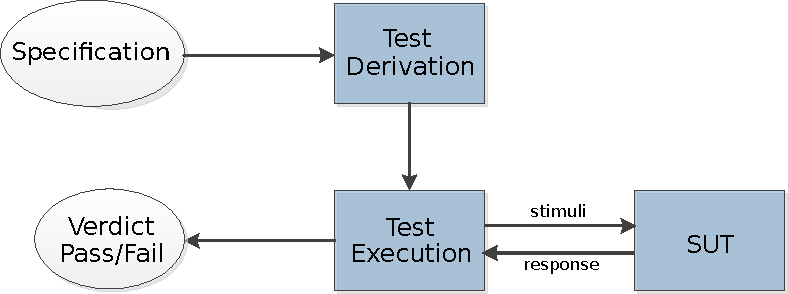
\includegraphics[width=0.75\textwidth]{model-based-testing.pdf}
  \end{center}
  \caption{A general model-based testing setup}
  \label{fig:model_based_testing}
\end{figure}

This type of model-based testing is called \textit{batch testing} or \textit{offline testing}. Another type of model-based testing is \textit{on-the-fly} testing. The main difference is that no test cases are derived, instead a transition in the model is chosen and tested on the system directly. The general architecture for this process is shown in Figure~\ref{fig:model_based_testing_on_the_fly}. An example of an on-the-fly testing is TorX~\cite{Tretmans:TorX}.

\begin{figure}[ht]
  \begin{center}
    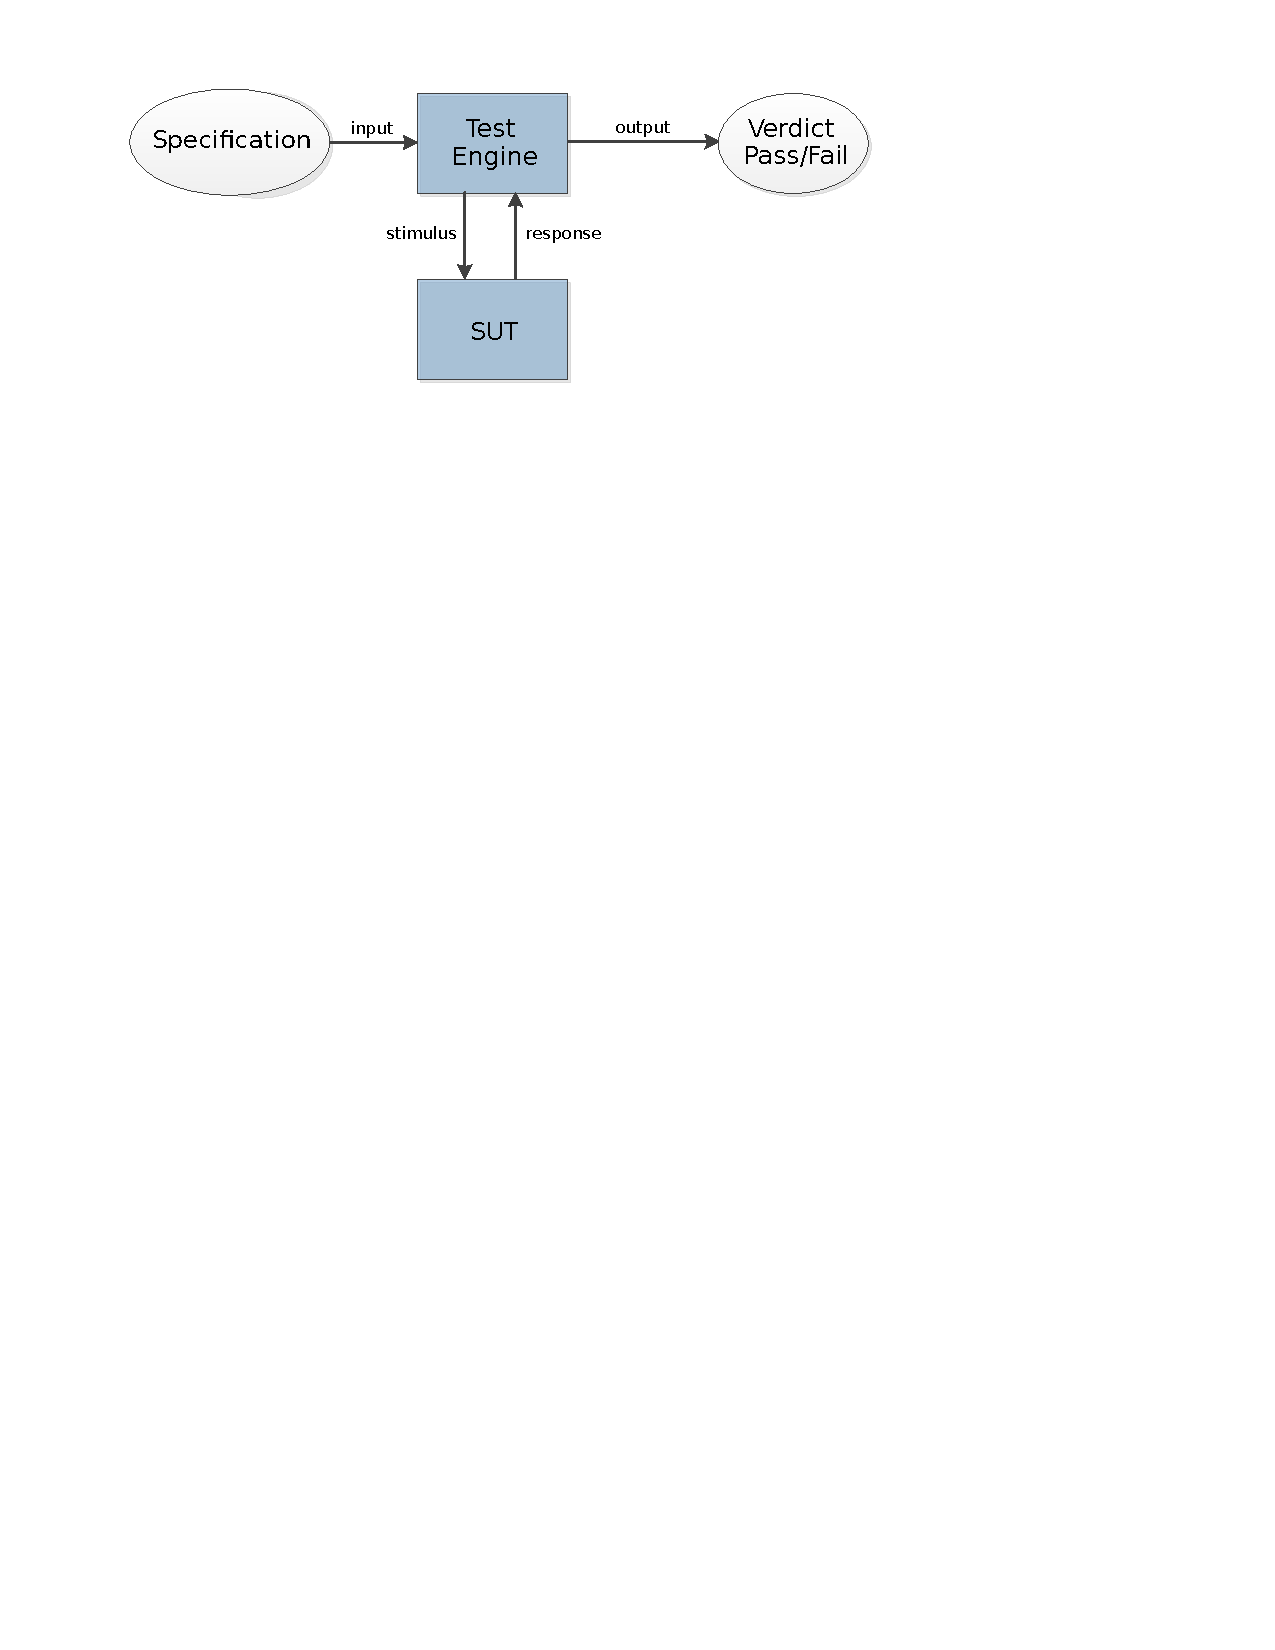
\includegraphics[width=0.75\textwidth]{mbt-on-the-fly.pdf}
  \end{center}
  \caption{A general 'on-the-fly' model-based testing setup}
  \label{fig:model_based_testing_on_the_fly}
\end{figure}\marginpar{A: Shrink font? V: Why?}

Variations of state machines and transition systems have been widely used as the underlying model for test generation. Other tools use the structure of data types to generate test data. 

The stucture of the rest of this section is as follows. First, previous work on model-based testing is given. Then, two types of models are introduced. These are basic formalisms useful to understand the models in the rest of the paper. Finally, the notion of \textit{coverage} is explained.

\subsection{Previous work}
Formal testing theory was introduced by De Nicola et al.~\cite{denicola:testing}. The input-output behavior of processes is investigated by series of tests. Two processes are considered equivalent if they pass exactly the same set of tests. This testing theory was first used in algorithms for automatic test generation by Brinksma~\cite{brinksma:testgeneration}. This led to the so-called \textit{canonical tester} theory. Tretmans gives a formal approach to protocol conformance testing (whether a protocol conforms to its specifications) in~\cite{Tretmans:conformancetesting} and an algorithm for deriving a sound and exhaustive test suite from a specification in~\cite{Tretmans:testgeneration}. A good overview of model-based testing theory and past research is given in "Model-Based Testing of Reactive Systems"~\cite{Broy:ModelBasedTesting}.

\subsection{Labelled Transition Systems}
A labelled transition system is a structure consisting of states with labelled transitions between them.
\vspace{5px}
\begin{definition}
A labelled transition system is a 4-tuple	$\langle Q, L, T, q_0\rangle$, where:
\begin{itemize}
\item $Q$ is a finite, non-empty set of states
\item $L$ is a finite set of labels
\item $T \in Q \times (L \cup \{\tau\}) \times Q$, with $\tau \notin L$, is the transition relation
\item $q_0 \in Q$ is the initial state.
\end{itemize}
We write $q \xrightarrow{\mu}q'$ if there is a transition labelled $\mu$ from state $q$ to state $q'$, i.e., $(q, \mu, q') \in T$. The informal idea of such a transition is that when the system is in state $q$ it may perform action $\mu$, and go to state $q'$. 
\end{definition}

\subsection{Input-Output Transition Systems}
A useful type of transition system for model-based testing is the Input-Output Transition System (IOTS) by Tretmans~\cite{Tretmans:testgeneration}. Assuming that implementations communicate with their environment via inputs and outputs, this formalism is useful for describing system behavior. IOTSs have the same definition as LTSs with one addition: each label $l \in L$ has a type $t \in T$, where $T = \{input, output\}$. Each label can therefore specify whether the action represented by the label is a possible input or an expected output of the system under test.

An example of such an IOTS is shown in Figure~\ref{fig:iots_example}. This system allows an input of 20 or 50 cents and then outputs tea or coffee accordingly. The inputs are preceded by a question mark, the outputs are preceded by an exclamation mark. This system is a specification of a coffee machine. A test case can also be described by an IOTS with special pass and fail states. A test case for the coffee machine is given in Figure~\ref{fig:iots_test}. The test case shows that when an input of '50c' is done, an output of 'coffee' is expected from the tested system, as this results in a 'pass' verdict. When the system responds with 'tea', the test case results in a 'fail' verdict. The pass and fail verdicts are two special states in the test case, which are sink states, i.e., once in either of those the test case cannot leave that state. 

Test cases should always reach a pass or fail state within finite time. This requirement ensures that the testing process halts.
\begin{figure}[ht]
  \begin{center}
    \subfloat[An IOTS]{\label{fig:iots_example}$\xymatrix{
    \bullet \ar[r]^{?50c} \ar[d]_{?20c} & \bullet \ar[d]^{\mathit{!coffee}} \\
    \bullet \ar[r]_{!tea}       & \bullet }$
}
    \subfloat[An IOTS test case]{\label{fig:iots_test}$\xymatrix{
    \bullet \ar[r]^{!50c} & \bullet \ar[r]^{\mathit{?coffee}} \ar[d]_{?tea} & {pass}\\
    & {fail}}$}
  \end{center}
  \caption{The specification of a coffee machine and a test case as an IOTS}
\end{figure}

\subsection{Coverage}\label{sec:coverage}
The number of tests that can be generated from a model is potentially infinite. Therefore, there must be a test selection strategy to maximize the quality of the tests while minimizing the time spent testing. Coverage statistics help with test selection. Such statistics indicate how much of the SUT is tested. When the SUT is a black-box, typical coverage metrics are state and transition coverage of the model~\cite{Lee:testing, Nachmanson:testing, Hasan:testing}.

As an example, let us calculate the coverage metrics of the IOTS test case example in~\ref{fig:iots_test}. The test case tests one path through the specification and passes through 3 out of 4 states and 2 out of 4 transitions. The state coverage is therefore 75\% and the transition coverage is 50\%.

Coverage statistics are calculated to indicate how adequately the testing has been performed~\cite{Zhu:coverage}. These statisics are therefore useful metrics for communicating how much of a system is tested.


  \section{Algebra}\label{sec:algebra}

Some basic concepts from algebra are described here. For a general introduction into logic we refer to~\cite{Huth:logic}.

A \textit{multi-sorted signature} $\langle \Sorts, \FunctionSymbols \rangle$ describes the function symbols and sorts of a formal language. $\FunctionSymbols$\newnot{symbol:FunctionSymbols} is a set of function symbols. $\Sorts$\newnot{symbol:Sorts} is a set of sorts. Each $\functionSymbol \in \FunctionSymbols$ has an arity $n \in \mathbb{N}$, where a function symbol with arity $n = 0$ is called a constant symbol. $\FunctionSymbols^i$ denotes the subset of $\FunctionSymbols$, with function symbols of arity $n = i$. The sort of a function symbol $\functionSymbol \in \FunctionSymbols$ with arity $n$ is given by $\sigma(f) = \sort_1 ... \sort_n+1$, with $\sort_i \in \Sorts$ for $1 \leq i \leq n$. $\Sorts_{n+1}$ is the return sort. In this report, $\Sorts =  \{\mathit{int, real, bool, string}\}$ denoting the integer, real, boolean and string sorts respectively. $\FunctionSymbols$ features the commonly used function symbols, which include, but not restricted by, '+', '*', '=', '<', '0', '1'.

An \textit{algebra} $\Algebra = \langle \mathbb{U}, \Functions\rangle$ has a non-empty set $\mathbb{U}$ of constants called a \textit{universe}, partitioned into $\mathbb{U}^\sort$ for each $\sort \in \Sorts$, and a set $\Functions$\newnot{symbol:Functions} of functions. A function $\function_\Algebra$ is typed $\mathbb{U}_\Algebra^{\sort_1} \times ... \mathbb{U}_\Algebra^{\sort_n} \rightarrow \mathbb{U}_\Algebra^{\sort_{n+1}}$, where $\sort_1 ... \sort_{n+1}$ is the sort of the function symbol given by the signature. For example, $<_\Algebra: \mathbb{U}_\Algebra^{int} \times \mathbb{U}_\Algebra^{int} \rightarrow \mathbb{U}_\Algebra^{bool}$ represents the 'less-than' comparison of two integers.
 
We define $\Variables = \Variables^{int} \uplus \Variables^{real} \uplus \Variables^{bool} \uplus \Variables^{string}$\newnot{symbol:Variables} to be the set of \textit{variables}. \textit{Terms} over $\DefinedVariables$, denoted $\Terms(\DefinedVariables)$\newnot{symbol:Terms}, are built from function symbols $\FunctionSymbols$ and variables $\DefinedVariables \subseteq \Variables$. The definition of a term is:
\vspace{8px}\\
$\begin{array}{lrlr}\term & ::= & \function(\term_1 ... \term_n) &\\ & | & x&\mathit{,\: where\: x\: is\: a\: constant.}\end{array}$
\vspace{8px}\\
We write $var(\term)$ to denote the set of variables appearing in a term $\term \in \Terms(\DefinedVariables)$. Terms $\term\in \Terms(\emptyset)$ are called ground terms. An example of a term $\term$ is $(x+(y-1))$, with $var(\term) = \{x,y\}$. The type of a term is given by:
\vspace{8px}\\
$\begin{array}{lll}\sortFunction: \term \mapsto & \sort       & \mathit{if}\: \term = x \in \Variables^\sort \\ 
 & \sort_{n+1} & \mathit{if}\: \term = \function(\term_1 ... \term_n) \mathit{\:and\:} \sortFunction(\function) = \sort_1 ... \sort_{n+1}\mathit{,\:provided\:} \sortFunction(\term_i) = \sort_i
\end{array}$
\vspace{8px}\\
The set of terms with return types $\mathbb{U}^{bool}$, is denoted as $\BooleanTerms(\Variables)$. An example is $(x < y)$, where the result is $\mathit{true}$ or $\mathit{false}$.

A \textit{term-mapping} is a function $\termMapping:\Variables \rightarrow \Terms(\Variables)$\newnot{symbol:termMapping}. A \textit{valuation} $\valuation$\newnot{symbol:valuation} is a function $\valuation:\Variables \rightarrow \mathbb{U}$ that assigns constants to variables. For example, given an algebra, $\valuation:\{(x \mapsto 1), (y \mapsto 2))\}$ assigns the constants 1 and 2 to the variables $x$ and $y$ respectively.
A valuation of a term given $\Algebra$ is defined by $\valuation(\function(\term_1 ... \term_n)) \mapsto \function_\Algebra(\valuation(\term_1) ... \valuation(\term_n))$. When every variable in a term is defined by a valuation, the term can be valuated to a constant. Therefore, when every variable in a term-mapping is defined by a valuation, a new valuation can be obtained. Formally, this is defined as: $\valuation_{after}:(\Variables \rightarrow \Terms(\Variables)) \rightarrow (\Variables \rightarrow \mathbb{U})$.

  \section{Symbolic Transition Systems}\label{sec:symbolic}
\textit{Symbolic Transition Systems} (STSs) combine a state oriented and data type oriented approach. These systems are used in practice in ATM and will therefore be part of GRATiS. In this section, previous work on STSs is given. The definitions of STSs and IOSTSs follow. An example of an IOSTS is then given. Next, the transformation of an STS to an LTS is explained and illustrated by an example. This transformation is useful when comparing STSs to systems that are not STSs. Finally, different coverage metrics on STSs are explained.

\subsection{Previous work}
STSs are introduced by Frantzen et al.~\cite{Frantzen:Symbolic}. This paper includes a detailed definition, on which the definition in section~\ref{sec:sts_definition} is based. The authors also give a sound and complete test derivation algorithm from specifications expressed as STSs. Deriving tests from a symbolic specification or \textit{Symbolic test generation} is introduced by Rusu et al.~\cite{rusu:symbolic}. Here, the authors use \textit{Input-Output Symbolic Transition Systems} (IOSTSs). These systems are very similar to the STSs in~\cite{Frantzen:Symbolic}. However, the definition of IOSTSs we will use in this report is based on the STSs by~\cite{Frantzen:Symbolic}. A tool that generates tests based on symbolic specifications is the STG tool, described in Clarke et al.~\cite{clarke:STG}.

\subsection{Definition}\label{sec:sts_definition}
An STS has \textit{locations} and \textit{switch relations}. If the STS represents a model of a software system, a location in the STS represents a state of the system, not including data values. A switch relation defines the transition from one location to another. The \textit{location variables} are a representation of the data values in the system. A switch relation has a \textit{gate}, which is a label representating the execution steps of the system. Gates have \textit{interaction variables}, which represent some input or output data value. Switch relations also have \textit{guards} and \textit{update mappings}. A guard is a term $\term \in \BooleanTerms(\Variables)$. The guard disallows using the switch relation when the valuation of the term results in $\mathit{false}$. When the valuation results in $\mathit{true}$, the switch relation of the guard is \textit{enabled}. An update mapping is a term-mapping of location variables. After the system switches to a new location, the variables in the update mapping will have the value corresponding to the valuation of the term.
\vspace{5px}
\begin{definition}
A Symbolic Transition System is a tuple $\langle \Locations,\initialLocation,\LocationVariables,\initializationFunction,\InteractionVariables,\Gates,\Switches\rangle$, where:
\begin{itemize}
\item $\Locations$\newnot{symbol:Locations} is a finite set of locations and $\initialLocation \in \Locations$\newnot{symbol:initialLocation} is the initial location.
\item $\LocationVariables \subseteq \Variables$\newnot{symbol:LocationVariables} is a finite set of location variables.
\item $\initializationFunction$\newnot{symbol:initializationFunction} is a term-mapping $\LocationVariables \rightarrow \Terms(\emptyset)$, representing the initialisation of the location variables.
\item $\InteractionVariables \subseteq \Variables$\newnot{symbol:InteractionVariables} is a set of interaction variables, disjoint from $\LocationVariables$.
\item $\Gates$\newnot{symbol:Gates} is a finite set of gates. The unobservable gate is denoted $\tau (\tau \notin \Gates)$; we write $\Gates_\tau$ for $\Gates \cup \{\tau\}$. The arity of a gate $\Gates\in\Gates_\tau$, denoted $arity(\Gates)$, is a natural number. The parameters of a gate $\Gates\in\Gates_\tau$, denoted $param(\Gates)$, are a tuple of length $arity(\Gates)$ of distinct interaction variables. We fix arity($\tau$) = 0, i.e. the unobservable gate has no interaction variables.
\item $\Switches \subseteq \Locations \times \Gates_\tau \times \BooleanTerms(\LocationVariables \cup \InteractionVariables) \times (\LocationVariables \rightarrow \Terms(\LocationVariables \cup \InteractionVariables)) \times \Locations$\newnot{symbol:Switches}, is the switch relation. We write $\location\xrightarrow{\Gates,\guard,\updateMapping}\location'$ instead of $(\location,\Gates,\guard,\updateMapping,\location')\in\Switches$, where $\guard$\newnot{symbol:guard} is referred to as the guard and $\updateMapping$\newnot{symbol:updateMapping} as the update mapping. We require $var(\guard) \cup var(\updateMapping \subseteq \LocationVariables \cup param(\Gates)$. We define $out(\location) \subset \Switches$ to be the outgoing switch relations from location $\location$.
\end{itemize}
\end{definition}

\subsection{Input-Output Symbolic Transition Systems}
An IOSTS can now easily be defined. The same difference between LTSs and IOTSs applies, namely each gate in an IOSTS has a type $\iotype \in \IOTypes$, where $\IOTypes = \{input, output\}$. As with IOSTSs, each gate is preceded by a '?' or '!' to indicate whether it is an input or an output respectively.

\subsection{Example}\label{sec:sts_example}
In Figure~\ref{fig:example_sts} the IOSTS of a simple board game is shown, where two players consecutively throw a die and move along four squares. The 'init' switch relation is a graphical representation of the variable initialization $\initializationFunction$. The values in the tuple of the IOSTS are defined as follows:

$\begin{array}{lcl}
\Locations & = & \{t, m\} \\
\initialLocation & = & t \\
\LocationVariables & = & \{T, P1, P2, D\} \\
\initializationFunction & = & \{T \mapsto 0, P1 \mapsto 0, P2 \mapsto 2, D \mapsto 0\} \\
\InteractionVariables & = & \{d, p, l\} \\
\Gates & = & \{?throw, !move\} \\
\Switches & = & \{t\xrightarrow{?throw, 1 <= d <= 6, D \mapsto d}m, \\
 & & m\xrightarrow{!move, T=1 \land l=(P1+D)\%4, P1 \mapsto l, T \mapsto 2}t, \\
 & & m\xrightarrow{!move, T=2 \land l=(P2+D)\%4, P2 \mapsto l, T \mapsto 1}t\}
\end{array}$

The variables $T, P1, P2$ and $D$ are the location variables symbolizing the player's turn, the positions of the players and the number of the die thrown respectively. The output gate $!move$ has $param = \langle p, l\rangle$ symbolizing which player moves to which location. The input gate $?throw$ has $param = \langle d\rangle$ symbolizing which number is thrown by the die. The switch relation with gate $?throw$ has the restriction that the number of the die thrown is between one and six and the update sets the location variable $D$ to the value of interaction variable $d$. The switch relations with gate $!move$ have the restriction that it must be the turn of the player moving and that the new location of the player is the number of steps ahead as thrown by the die. The update mapping sets the location of the player to the correct value and passes the turn to the next player. In Figure~\ref{fig:example_sts} the gates, guards and updates are separated by pipe symbols '|' respectively.

\begin{figure}[ht]
  \begin{center}
    $\xymatrix{
   \ar[rrrrr]^{init\:|\:true\:|\:T\mapsto 1,\:P1\mapsto 0,\:P2\mapsto 2,\:D\mapsto 0} &&&&& {t} \ar[rrrrrrrr]^{?throws(d:N)\,|\,1\,<=\,d\,<=\,6\,|\,D\mapsto d} &&&&&&&& {m} \ar@/_2pc/[llllllll]_{!move(p:N,l:N)\: |\: T=1 \:\land\: p=1 \:\land\: l = (P1+D)\%4\:|\:P1\mapsto l,\:T\mapsto 2} \ar@/^2pc/[llllllll]^{!move(p:N,l:N) \:|\: T=2 \:\land\: p=2 \land l = (P2+D)\,\%4\:|\: P2\mapsto l,\:T\mapsto 1}
}$

  \end{center}
  \caption{The STS of a board game example}
  \label{fig:example_sts}
\end{figure}

\subsection{STS to LTS mapping}\label{sec:sts_lts_trafo}
Consider an STS $J$ and an LTS $K$. There exists a mapping from the location and location variable valuations to the states of $K$ and from the switch relations and variable valuations of $J$ to the transitions of $K$, such that $K$ is an expansion of $J$. These relations are defined as follows:
$\begin{array}{ll}
\StsExpansionMapping_\States: & (\Locations \times (\LocationVariables \rightarrow \mathbb{U})) \rightarrow \States \\
\StsExpansionMapping_\Labels: & (\Gates \times (\InteractionVariables \rightarrow \mathbb{U})) \rightarrow \Labels \\
\StsExpansionMapping_\Transitions: & (\location\xrightarrow{\gate,\guard,\updateMapping}\location', \valuation: ((\LocationVariables \cup \InteractionVariables) \rightarrow \mathbb{U})) \mapsto (\StsExpansionMapping_\States(\location, \valuation \restriction \LocationVariables) \xrightarrow{\StsExpansionMapping_\Labels(\gate, \valuation \restriction\InteractionVariables)} \StsExpansionMapping_\States(\location', \valuation_{after}(\updateMapping)))
\end{array}$

\begin{comment}
These relations are constructed as follows: for a switch relation $r$ from location $A$ to location $B$, a valuation of the location variables $\nu_l$ and interaction variables $\nu_i$, $\mu_l:(A,\nu_l)$ maps to a state $q$, where $q$ is the source state of a transition $t$, if the result of the valuation $\nu:(\phi$ of $r, \nu_l \cup \nu_i)$ is true. $\nu_{l_new}$ is the new valuation of the location variables constructed by the valuation of $\rho$ of $r$. Then, the target state $q'$ of $t$ is the state mapped by $\mu_l:(B,\nu_{l_new}$). The label of $t$ is a textual representation of $\Gates$ of $r$ and $\nu_i$. Applying this rule for the topology to all locations, switch relations and concrete values for the variables, results in $L$. The start state $q0$ of $L$ is the state mapped by $\mu_l:(l_0,\initializationFunction)$. All states not reachable from $q0$ are removed from $L$.
\end{comment}

When the number of possible valuations for $\LocationVariables$ and $\InteractionVariables$ and the number of locations in an STS is considered to be finite, the transformation is always possible to an LTS with finite number of states.

An example of this transformation is shown in Figure~\ref{fig:example_trafo}. The label 'do(1)' in the LTS is a textual representation of the gate 'do' plus a valuation of the interaction variable 'd'. The transformation of a switch relation and concrete values to a transition is also called \textit{instantiating} the switch relation. Another term we will use for a switch relation with a set of concrete data values is an \textit{instantiated switch relation}.

\begin{figure}[ht]
  \begin{center}
    \subfloat[The STS]{\label{fig:trafo_sts}$\xymatrix{
   \ar[d]^{init\,|\,true\,|\,N\,:=\,0;} \\
   \bullet \ar@/^/[d]^{do(d:N)\,|\,1\,<=\,n\,<=\,2\,|\,N\,:=\,n} \\
   \bullet \ar@/^/[u]^{sub(i:N)\,|\,1\,<=\,i\,<=\,2\,|\,N\,:=\,N\,-\,i}}$
}\hspace{20px}
    \subfloat[The LTS]{\label{fig:trafo_lts}$\xymatrix{
\fbox{$\location_0, N=2$} & \ar[r] & \fbox{$\location_0, N=0$} \ar@/^/[ddll]^{do(1)} \ar@/^/[ddrr]^{do(2)} && \\ \\
 \fbox{$\location_1, N=1$} \ar@/^/[uurr]^{sub(1)} \ar@/^/[ddrr]^{sub(2)} && \fbox{$\location_0, N=1$} \ar[ll]^{do(1)} \ar@/^/[rr]^{do(2)} && \fbox{$\location_1, N=2$} \ar@/^/[ll]^{sub(1)} \ar@/^/[uull]^{sub(2)} \\\\
 && \fbox{$\location_0, N=-1$} \ar@/^/[uull]^{do(1)} \ar[uurr]^{do(2)}}$
}
  \end{center}
  \caption{An example of a transformation of an STS to an LTS}
  \label{fig:example_trafo}
\end{figure}

\subsection{Coverage}\label{sec:sts_coverage}
The simplest metric to describe the coverage of an STS is the location and switch-relation coverage, which express the percentage of locations and switch relations tested in the test run. Measuring state and transition coverage of an STS is possible using the LTS resulting from the STS transformation. However, this metric is not always useful, because the number of states and transitions in the LTS depend on the number of unique combinations of concrete values of the variables in the STS. This is potentially very large. For example, when the guards of the switch relations in Figure~\ref{fig:trafo_sts} are removed, the transformation leads to an LTS with a state and transition for each possible value of an integer. It is often infeasable to test every data value in the STS. The most interesting data values to test can be found by \textit{boundary-value analysis} and \textit{equivalence partitioning}. For an explanation of these terms we refer to~\cite{Myers:2004}.\marginpar{A:Explain! (example) V: Ik denk eigenlijk niet dat deze technieken relevant gaan zijn uiteindelijk} Boundary-value analysis was found to be most effective by Reid~\cite{Reid:partitioning} in fault detection.

\textit{Data coverage} expresses the percentage of data tested in the test run, considering data to be similar if located in the same partition and a better representative of the partition if located close to the partition boundary. These properties of the tested data affect the data coverage percentage.

  \section{Graph Grammars}\label{sec:graph}
A \textit{graph grammar} is composed of a start graph and a set of transformation rules. The start graph describes the system in its initial state. The transformation rules describe what changes are made to the graph, resulting in a new graph which describes the system in its new state. The definition is as follows.

\begin{definition}
A graph grammar is a tuple $\langle G, R\rangle$, where:
\begin{itemize}
  \item $G$ is the start graph
  \item $R$ is a set of graph transformation rules
\end{itemize}
\end{definition} 

The rest of this section is ordered as follows: first, graphs and graph morphisms are explained. This is then used to explain graph transformation rules, followed by the definition of a graph grammar. Then, the definition of a \textit{Graph Transition System} (GTS) is given. An example of a graph grammar and a GTS is then given. Finally, a method for transforming a GTS to an STS is given. For a more detailed overview of graph grammars, we refer to~\cite{Rensink:graph_grammars, Heckel2006187, Andries1999}.

\subsection{Graphs \& morphisms}
\begin{definition}
A graph is a tuple $\langle L, N, E\rangle$, where:
\begin{itemize}
  \item $L$ is a set of labels
  \item $N$ is a set of nodes, where each $n \in N$ has a label $l \in L$
  \item $E$ is a set of edges, where each $e \in E$ has a label $l \in L$ and nodes $source,target \in N$
\end{itemize}
\end{definition}

A graph $H$ has an \textit{occurrence} in a graph $G$, denoted by $H \rightarrow G$, if there is a mapping from the nodes and the edges of $H$ to the nodes and the edges of $G$ respectively. Such a mapping is called a \textit{morphism}. An element $e$ in graph $H$ is then said to have an \textit{image} in graph $G$ and $e$ is a \textit{pre-image} of the image. A graph $H$ has a partial morphism to a graph $G$ if there are elements in $H$ without an image in $G$.

\subsection{Graph transformation rules}
\begin{definition}
A transformation rule is a tuple $\langle \mathit{LHS}, \mathit{NAC}, \mathit{RHS}, \mathit{M}\rangle$, where:
\begin{itemize}
  \item $\mathit{LHS}$ is a graph representing the left-hand side of the rule
  \item $\mathit{NAC}$ is a set of graphs representing the negative application conditions
  \item $\mathit{RHS}$ is a graph representing the right-hand side of the rule
  \item $\mathit{M_{RHS}}$ is a partial morphism of $\mathit{LHS}$ to $\mathit{RHS}$ 
  \item $\mathit{M_{NAC}}$ are partial morphisms of $\mathit{LHS}$ to each $n \in \mathit{NAC}$
\end{itemize}
\end{definition}

A rule $R$ is applicable on a graph $G$ if its $\mathit{LHS}$ has an occurrence in $G$ and $\not\ exists n \in \mathit{NAC}$ such that $n$ has an occurence in $G$ and $\forall e \in \mathit{LHS}$, if $e$ has an image $i$ in $n$ and an image $j$ in $G$, then $j$ should be an image of $j$. This 'applicability' as defined here is refered to as a rule \textit{match}. After the rule match is applied to the graph, all elements in $\mathit{LHS}$ not part of $\mathit{M_{RHS}}$, i.e. they do not have an image in $\mathit{RHS}$, are removed from $G$ and all elements in $\mathit{RHS}$ not part of $\mathit{M_{RHS}}$, i.e. they do not have a pre-image in $\mathit{LHS}$, are added to $G$.

\subsection{Graph Transition Systems}
By repeatedly applying graph transformation rules to the start graph and all its consecutive graphs, a graph grammar can be explored to reveal a \textit{Graph Transition System} (GTS). This transition system consists of \textit{graph states} connected by \textit{rule transitions}.

\begin{definition}
A graph transition system is an 8-tuple	$\langle S, L, T, G, R, M_G, M_R, s0\rangle$, where:
\begin{itemize}
\item $S$ is a finite, non-empty set of graph states
\item $L$ is a finite set of labels.
\item $T \in S \times (L \cup \{\tau\}) \times S$, with $\tau \notin L$, is the rule transition relation.
\item $G$ is a set of graphs.
\item $R$ is a set of rules.
\item $M_G$ is a mapping $\forall s \in S . s \mapsto g \in G \land \not\exists s' \in S . s \neq s' \land s' \mapsto g \in M_G$
\item $M_R$ is a mapping $\forall t \in T . t \mapsto r \in R \land \not\exists t' \in T . t \neq t' \land t' \mapsto r \in M_R$
\item $s0 \in s$ is the initial graph state.
\end{itemize}
We write $s \xrightarrow{\mu}s'$ if there is a rule transition labelled $\mu$ from state s to state s', i.e., $(s, \mu, s') \in T$.
\end{definition}

These systems are very similar to LTSs. A GTS can be transformed to an LTS by omitting the graphs, rules and mappings.

\subsection{Example}\label{sec:gts_example}
Figure \ref{fig:gts} shows an example of the start graph and one rule of a graph grammar. $\mathit{M_{RHS}}$ maps the $A$ and $B$ nodes in $\mathit{LHS}$ to the A and B nodes in $\mathit{RHS}$ respectively. $\mathit{M_{NAC}}$ maps the $A$ node in $\mathit{LHS}$ to the $A$ node in both graphs in $\mathit{NAC}$. The a-edge in $\mathit{LHS}$ is mapped to the a-edge in the first $\mathit{NAC}$. The $\mathit{LHS}$ of the rule has an occurrence in the start graph, as the $A$ and $B$ nodes connected by the a-edge exist in both graphs. None of the graphs in the $\mathit{NAC}$ have an occurrence in the start graph, because the $C$ node does not exist in the start graph. The new graph after applying the rule is in Figure~\ref{fig:gg_result}.

\begin{figure}[ht]
  \begin{center}
    \subfloat[The start graph]{\label{fig:gg_graph}$\xymatrix{
   \fbox{A} \ar[r]^{a} & \fbox{B}
}$
}\hspace{20px}
    \subfloat[The LHS]{\label{fig:gg_lhs}$\xymatrix{
   \fbox{A} \ar[r]^{a} & \fbox{B}
}$
}\hspace{20px}
    \subfloat[The first NAC]{\label{fig:gg_nac1}$\xymatrix{
   \fbox{A} \ar[r]^{a} & \fbox{C}
}$
}\hspace{20px}
    
    \subfloat[The second NAC]{\label{fig:gg_nac2}$\xymatrix{
   \bullet \ar@(dl,dr)[]_{A} \ar[r]^{b} & \bullet \ar@(dl,dr)[]_{C}
}$
}\hspace{20px}
    \subfloat[The RHS]{\label{fig:gg_rhs}$\xymatrix{
   \bullet \ar@(dl,dr)[]_{A} \ar[r]^{b} & \bullet \ar@(dl,dr)[]_{B}
}$
}\hspace{20px}
    \subfloat[The result]{\label{fig:gg_result}$\xymatrix{
   \bullet \ar@(dl,dr)[]_{A} \ar[r]^{b} & \bullet \ar@(dl,dr)[]_{B}
}$
}
  \end{center}
  \caption{An example of a graph grammar}
  \label{fig:gts}
\end{figure}

  \section{Tooling}\label{sec:tooling}

\subsection{ATM}\label{sec:descriptionaxini}
ATM is a web-based application, developed in the Ruby on Rails framework. It is used to test the software of several big companies in the Netherlands since 2006. It is under continuous development by Axini.

The architecture is shown graphically in Figure~\ref{fig:axini_tool}. It has a similar structure to the on-the-fly model-based testing tool architecture in Figure~\ref{fig:model_based_testing_on_the_fly}.

\begin{figure}[h!]
  \begin{center}
    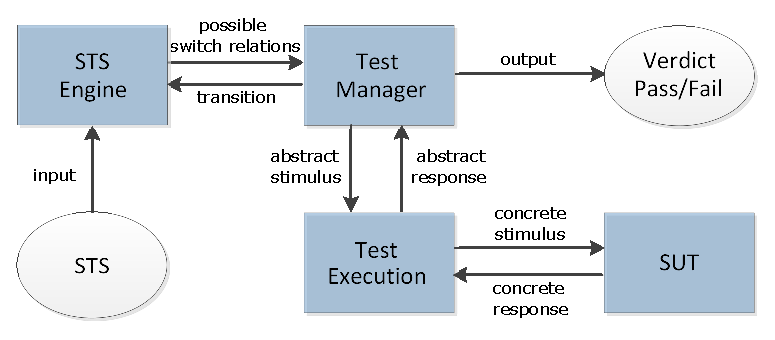
\includegraphics[width=0.75\textwidth]{axini_tool.eps}
  \end{center}
  \caption{Architecture of ATM}
  \label{fig:axini_tool}
\end{figure}

The tool functions as follows: 
\begin{enumerate}
  \item An STS is given to an STS Engine, which passes the possible switch relations from the current state to the Test Manager.
  \item The Test Manager chooses a switch relation and the data values, based on a test strategy. In the LTS in the STS-to-LTS transformation, this choice is represented by one transition. 
  \item The label of the transition is given to the Test Execution component as an \textit{abstract stimulus}. The term abstract is used here to indicate that the transition is specific to the model. It represents some computation steps taken in the SUT. For instance, a transition with label 'connect?' is an abstract stimulus of the actual setup of a TCP connection between two distributed components of the SUT. 
  \item The translation of an abstract stimulus to a concrete stimulus is done by the Test Execution component. This component provides the stimulus to the SUT. When the SUT responds, the Test Execution component translates this response to an abstract response. For instance, the Test Execution component receives an HTTP response that the TCP connect was succesful. This is a concrete response, which the Test Execution component translates to an abstract response, such as a transition with label 'ok!'. The Test Manager is notified with this abstract response.
  \item The Test Manager updates the STS Engine on which transition was chosen as stimulus and which transition was detected based on the response of the SUT. If this latter transition is possible according to the model, the Test Manager gives a pass verdict for this test. Otherwise, the result is a fail verdict.
\end{enumerate}

\subsection{GROOVE}\label{sec:descriptiongroove}
GROOVE is an open source, graph-based modelling tool in development at the University of Twente since 2004. It has been applied to several case studies, such as model transformations and security and leader election protocols~\cite{Ghamarian:GROOVE}.

The architecture of the GROOVE tool is shown graphically in Figure~\ref{fig:groove_tool}. A GTS is given as input to a Rule Applier component, which determines the possible rule transitions. An Exploration Strategy can be started or the user can explore the states manually using the GUI. These components request the possible rule transitions and respond with the chosen rule transition (based on the exploration strategy or the user input). The Exploration Strategy can do an exhaustive search, resulting in a GTiS. The graph states and rule transitions in this GTiS can then be inspected using the GUI.

\begin{figure}[h]
  \begin{center}
    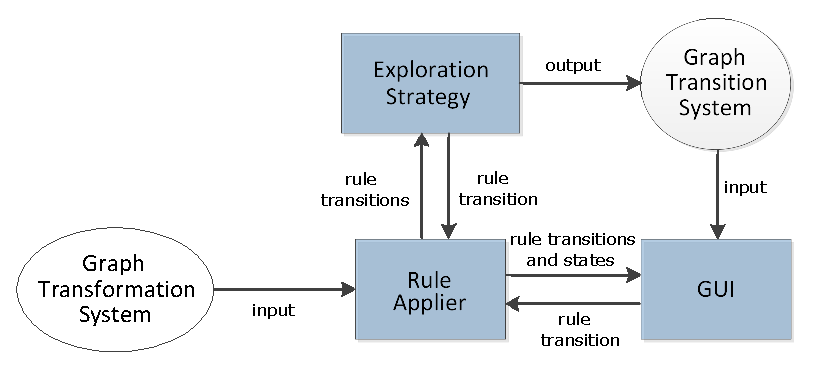
\includegraphics[width=0.75\textwidth]{groove_tool.eps}
  \end{center}
  \caption{The GROOVE Tool}
  \label{fig:groove_tool}
\end{figure}

%GROOVE provides parameters for the labels on the transitions in a GTiS by indicating which node(s) in a rule should be the parameter(s). 
\subsection{Comparison of the examples}\label{sec:comparison}
The models of the boardgame example in Figures~\ref{fig:example_sts} and \ref{fig:example_groove} are very different. In this section the STS and the GTS of the example are compared.

\subsubsection{Comparison of behavior}
The GTS of the boardgame example has a number of consecutive transitions when a player moves. The $move$ rule puts the \textbf{Player} on the next \textbf{Location} and lowers the remaining 'moves' by one. This is different from the STS, which updates the location variable in one transition. The effect is that the behavior of both systems is different; one specifies the movement of a \textbf{Player} as: "Player p moves to Location l", the other as: "The Player with the turn moves to the next Location". Which behavior is required when this boardgame would be tested depends on the implementation of the game. However, to show the power of the GTS formalism, Figure~\ref{fig:example_groove2} shows the GTS with the same behavior as the STS. It models the location as a variable and updates this variable in one transition. It also identifies the \textbf{Players} by giving them a number.

\begin{figure}[h]
  \begin{center}
    \subfloat[The start graph]{\label{fig:example_groove_start2}% To use this figure in your LaTeX document
% import the package groove/resources/groove2tikz.sty
%
% Special colors
\begin{tikzpicture}[
% Special color styles
scale=\tikzscale]
\node[node] (n9)  at (1.975, -0.725) {\ml{\textbf{Location}\\field = 1\\field = 3\\field = 2\\field = 0}};
\node[node] (n0)  at (0.825, -0.875) {\ml{\textbf{Die}\\canThrow = 1\\canThrow = 2\\canThrow = 3\\canThrow = 4\\canThrow = 5\\canThrow = 6}};
\node[node] (n11)  at (2.965, -0.660) {\ml{\textbf{Player}\\\textit{turn}\\at = 0\\number = 1}};
\node[node] (n12)  at (3.945, -0.595) {\ml{\textbf{Player}\\at = 2\\number = 2}};
\userdefinedmacro
\end{tikzpicture}
\renewcommand{\userdefinedmacro}{\relax}
}\quad
    \subfloat[The throw rule]{\label{fig:example_groove_throw2}% To use this figure in your LaTeX document
% import the package groove/resources/groove2tikz.sty
%
% Special colors
\begin{tikzpicture}[
% Special color styles
scale=\tikzscale]
\node[node] (n5)  at (1.595, -1.295) {\ml{\textbf{Die}}};
\node[nacnode, attr] (n2)  at (0.495, -1.325) {\ml{\textbf{int}}};
\node[node, attr] (n4)  at (1.605, -0.415) {\ml{\textbf{int}}};
\node[node] (n1)  at (0.545, -0.470) {\ml{\textbf{Player}\\\textit{turn}}};
\path[edge](n5.north -| 1.605, -0.415) -- node[lab]{canThrow} (n4) ;
\path[newedge](n1.east |- 1.605, -0.415) -- node[newlab]{throws} (n4) ;
\path[nacedge](n1.south -| 0.495, -1.325) -- node[naclab]{throws} (n2) ;
\userdefinedmacro
\end{tikzpicture}
\renewcommand{\userdefinedmacro}{\relax}
}
    \subfloat[The move rule]{\label{fig:example_groove_move2}% To use this figure in your LaTeX document
% import the package groove/resources/groove2tikz.sty
%
% Special colors
\begin{tikzpicture}[
% Special color styles
scale=\tikzscale]
\node[node, attr] (n1)  at (0.965, -1.520) {\ml{\textbf{int}}};
\node[node] (n0)  at (1.070, -0.680) {\ml{\textbf{Player}\\{\color{\blue}\textit{$-$ turn}}\\{\color{\green}at := (at $+$ throws) \% 4}}};
\node[node] (n2)  at (2.540, -0.660) {\ml{\textbf{Player}\\{\color{\green}\textit{$+$ turn}}}};
\path[deledge](n0.south -| 0.965, -1.520) -- node[dellab]{throws} (n1) ;
\path[edge, -](n2.west |- 1.070, -0.680) -- node[lab]{\textit{!=}} (n0) ;
\userdefinedmacro
\end{tikzpicture}
\renewcommand{\userdefinedmacro}{\relax}
}
  \end{center}
  \caption{Another GTS model of the board game example}
  \label{fig:example_groove2}
\end{figure}

The new GTS loses many advantages by structuring it in this way: the overview of the board is gone, the rules are less visual and extending the locations in different directions is much harder. On the other hand, there are less rules and the graphs are more compact. However, when finding the GTiS corresponding to this GTS, the labels of the transitions of that GTiS do not reflect the 'move(p:N, l:N)' label of the STS. This should be done by marking the correct nodes as described in section~\ref{sec:gts_example}. The problem is that the result of the equation in the 'move' rule is only derived when the rule is applied. Figure~\ref{fig:move3} shows a rule where the equation is shown graphically. The die roll, connected by the 'throws' edge, and the number of the \textbf{Location} the \textbf{Player} is at are added. The result is represented by the \textbf{int} node connected by the 'add' edge. This result modulo 4 is represented by the \textbf{int} node connected by the 'mod' edge. This node is marked as the second parameter, the number of the \textbf{Player} is marked as the first parameter. This labels the transitions with which player moves to which location.

\begin{figure}[h]
  \begin{center}
    % To use this figure in your LaTeX document
% import the package groove/resources/groove2tikz.sty
%
% Special colors
\begin{tikzpicture}[
% Special color styles
scale=\tikzscale]
\node[node] (n0)  at (1.985, -0.650) {\ml{\textbf{Player}\\{\color{\blue}\textit{$-$ turn}}}};
\node[node, attr] (n8)  at (2.405, -2.195) {\ml{\textbf{int}}};
\node[node, attr] (n5)  at (0.375, -0.655) {\ml{\textbf{int}}};
\node[parnode] (n5p)  at (n5.north west) {0};
\node[node, attr] (n4)  at (0.965, -1.485) {\ml{\textbf{int}}};
\node[node, prod] (n9)  at (3.445, -2.185) {\ml{\textit{$\pi$1 = 4}}};
\node[node] (n2)  at (3.455, -0.640) {\ml{\textbf{Player}\\{\color{\green}\textit{$+$ turn}}}};
\node[node, attr] (n10)  at (3.425, -1.395) {\ml{\textbf{int}}};
\node[parnode] (n10p)  at (n10.north west) {1};
\node[node, attr] (n7)  at (1.935, -1.475) {\ml{\textbf{int}}};
\node[node, prod] (n6)  at (1.395, -2.205){};
\path[edge] (n9)  -- node[lab]{mod} (n10) ;
\path[edge] (n6)  -- node[lab]{$\pi$0} (n4) ;
\path[edge](n0.west |- 0.375, -0.655) -- node[lab]{number} (n5) ;
\path[deledge](n0.south -| 1.935, -1.475) -- node[dellab]{at} (n7) ;
\path[deledge] (n0)  -- node[dellab]{throws} (n4) ;
\path[edge] (n9)  -- node[lab]{$\pi$0} (n8) ;
\path[edge, -](n2.west |- 1.985, -0.650) -- node[lab]{\textit{!=}} (n0) ;
\path[edge] (n6)  -- node[lab]{add} (n8) ;
\path[edge] (n6)  -- node[lab]{$\pi$1} (n7) ;
\path[newedge] (n0)  -- node[newlab]{at} (n10) ;
\userdefinedmacro
\end{tikzpicture}
\renewcommand{\userdefinedmacro}{\relax}

  \end{center}
  \caption{An alternative move rule}
  \label{fig:move3}
\end{figure}

\subsubsection{Comparison of Transition Systems}
The GTiS of a GTS can be found using GROOVE and the STS can be transformed to an LTS. The two GTSs and the STS of the board game example result in three transition systems which can be compared.

The GTS from Figure~\ref{fig:example_groove} generates a GTiS with 32 states with 52 transitions, which can be seen visually in Figure~ \ref{fig:statespace_groove1}. The GTS from Figure \ref{fig:example_groove2}, using the 'move' rule from Figure~\ref{fig:move3}, generates 224 states with 384 transitions, shown as GTiS in Figure~\ref{fig:statespace_groove2}. The reason of the difference in number of states and transitions is that the board is circular: to the first GTS, the players being at locations 1 and 3 is the same as them being at locations 2 and 4. However, this is not the same to the second GTS. Also, for the first GTS it does not matter which \textbf{Player} node is at a \textbf{Location} node; they are the same apart from which \textbf{Player} has the 'turn'. As an example, consider the start graph in Figure~\ref{fig:example_groove}. If both players throw a '1' and move to the next location, the state is as shown in Figure~\ref{fig:symmetry_example}. Both states are symmetrical and therefore they are the same state. This leads to a \textit{symmetry reduction} of the statespace for the first GTS.

\begin{figure}[h]
  \begin{center}
    % To use this figure in your LaTeX document
% import the package groove/resources/groove2tikz.sty
%
% Special colors
\begin{tikzpicture}[
% Special color styles
scale=\tikzscale]
\node[node] (n9)  at (4.245, -1.375) {\ml{\textbf{Location}}};
\node[node, bold] (n0)  at (1.585, -0.865) {\ml{\textbf{Die}\\canThrow = 1\\canThrow = 2\\canThrow = 3\\canThrow = 4\\canThrow = 5\\canThrow = 6}};
\node[node] (n7)  at (5.625, -1.935) {\ml{\textbf{Location}}};
\node[node, bold] (n11)  at (3.055, -0.520) {\ml{\textbf{Player}\\\textit{turn}}};
\node[node] (n12)  at (5.615, -0.525) {\ml{\textbf{Player}}};
\node[node] (n8)  at (2.995, -1.895) {\ml{\textbf{Location}}};
\node[node] (n10)  at (4.265, -2.455) {\ml{\textbf{Location}}};
\path[edge] (n10)  -- node[lab]{next} (n8) ;
\path[edge] (n7)  -- node[lab]{next} (n10) ;
\path[edge] (n9)  -- node[lab]{next} (n7) ;
\path[edge] (n11)  -- node[lab]{at} (n9) ;
\path[edge] (n8)  -- node[lab]{next} (n9) ;
\path[edge] (n12)  -- node[lab]{at} (n10) ;
\userdefinedmacro
\end{tikzpicture}
\renewcommand{\userdefinedmacro}{\relax}

  \end{center}
  \caption{An example of a state symmetrical with the state in Figure~\ref{fig:example_groove}}
  \label{fig:symmetry_example}
\end{figure}

The LTS where the STS in Figure~\ref{fig:example_sts} is transformed to has 224 states and 384 transitions. This is calculated by taking all possibilities of the data values except for the die roll. This leads to 32 states ($4 \times 4 \times 2$). These 32 'throw' states each have 6 'throw?' transitions to a 'move' state, thus there are 192 'move' states. The 'move' states only have one transition back to a 'throw' state. There are $6 \times 32 + 192 \times 1 = 384$ transitions.

\begin{figure}[h]
  \begin{center}
    \resizebox{\textwidth}{!}{% To use this figure in your LaTeX document
% import the package groove/resources/groove2tikz.sty
%
% Special colors
\begin{tikzpicture}[
% Special color styles
scale=\tikzscale]
\node[node, start] (s0)  at (4.240, -0.155) {\ml{\textit{s0}}};
\node[node] (s1)  at (0.590, -0.865) {\ml{\textit{s1}}};
\node[node] (s2)  at (1.870, -0.865) {\ml{\textit{s2}}};
\node[node] (s3)  at (5.130, -0.865) {\ml{\textit{s3}}};
\node[node] (s4)  at (6.050, -0.865) {\ml{\textit{s4}}};
\node[node] (s5)  at (6.970, -0.865) {\ml{\textit{s5}}};
\node[node] (s6)  at (7.890, -0.865) {\ml{\textit{s6}}};
\node[node] (s7)  at (0.590, -1.575) {\ml{\textit{s7}}};
\node[node] (s8)  at (1.870, -1.575) {\ml{\textit{s8}}};
\node[node] (s9)  at (5.130, -1.575) {\ml{\textit{s9}}};
\node[node] (s10)  at (6.055, -1.575) {\ml{\textit{s10}}};
\node[node] (s11)  at (6.975, -1.575) {\ml{\textit{s11}}};
\node[node] (s12)  at (7.895, -1.575) {\ml{\textit{s12}}};
\node[node] (s13)  at (0.595, -2.285) {\ml{\textit{s13}}};
\node[node] (s14)  at (1.875, -2.285) {\ml{\textit{s14}}};
\node[node] (s15)  at (5.135, -2.285) {\ml{\textit{s15}}};
\node[node] (s16)  at (6.055, -2.285) {\ml{\textit{s16}}};
\node[node] (s17)  at (6.975, -2.285) {\ml{\textit{s17}}};
\node[node] (s18)  at (7.895, -2.285) {\ml{\textit{s18}}};
\node[node] (s19)  at (0.595, -2.995) {\ml{\textit{s19}}};
\node[node] (s20)  at (1.875, -2.995) {\ml{\textit{s20}}};
\node[node] (s21)  at (2.665, -2.995) {\ml{\textit{s21}}};
\node[node] (s22)  at (3.915, -1.325) {\ml{\textit{s22}}};
\node[node] (s23)  at (4.625, -3.025) {\ml{\textit{s23}}};
\node[node] (s24)  at (5.635, -2.995) {\ml{\textit{s24}}};
\node[node] (s25)  at (6.625, -2.995) {\ml{\textit{s25}}};
\node[node] (s26)  at (5.145, -3.665) {\ml{\textit{s26}}};
\node[node] (s27)  at (0.595, -3.705) {\ml{\textit{s27}}};
\node[node] (s28)  at (1.865, -3.845) {\ml{\textit{s28}}};
\node[node] (s29)  at (2.855, -3.395) {\ml{\textit{s29}}};
\node[node] (s30)  at (3.435, -1.295) {\ml{\textit{s30}}};
\node[node] (s31)  at (0.595, -4.415) {\ml{\textit{s31}}};
\path[edge] (s0)  -- node[lab]{throws(3)} (s1) ;
\path[edge] (s0)  -- node[lab]{throws(2)} (s2) ;
\path[edge] (s0)  -- node[lab]{throws(1)} (s3) ;
\path[edge] (s0)  -- node[lab]{throws(5)} (s4) ;
\path[edge] (s0)  -- node[lab]{throws(6)} (s5) ;
\path[edge] (s0)  -- node[lab]{throws(4)} (s6) ;
\path[edge](s1.south -| 0.590, -1.575) -- node[lab]{move(1)} (s7) ;
\path[edge](s2.south -| 1.870, -1.575) -- node[lab]{move(1)} (s8) ;
\path[edge](s3.south -| 5.130, -1.575) -- node[lab]{move(1)} (s9) ;
\path[edge](s4.south -| 6.055, -1.575) -- node[lab]{move(1)} (s10) ;
\path[edge](s5.south -| 6.975, -1.575) -- node[lab]{move(1)} (s11) ;
\path[edge](s6.south -| 7.895, -1.575) -- node[lab]{move(1)} (s12) ;
\path[edge](s7.south -| 0.595, -2.285) -- node[lab]{move(1)} (s13) ;
\path[edge](s8.south -| 1.875, -2.285) -- node[lab]{move(1)} (s14) ;
\path[edge](s9.south -| 5.135, -2.285) -- node[lab]{nextTurn()} (s15) ;
\path[edge](s10.south -| 6.055, -2.285) -- node[lab]{move(1)} (s16) ;
\path[edge](s11.south -| 6.975, -2.285) -- node[lab]{move(1)} (s17) ;
\path[edge](s12.south -| 7.895, -2.285) -- node[lab]{move(1)} (s18) ;
\path[edge](s13.south -| 0.595, -2.995) -- node[lab]{move(1)} (s19) ;
\path[edge](s14.south -| 1.875, -2.995) -- node[lab]{nextTurn()} (s20) ;
\path[edge] (s15)  -- node[lab]{throws(3)} (s21) ;
\path[edge] (s15)  -- node[lab]{throws(2)} (s22) ;
\path[edge] (s15)  -- node[lab]{throws(1)} (s23) ;
\path[edge] (s15)  -- node[lab]{throws(5)} (s24) ;
\path[edge] (s15)  -- node[lab]{throws(6)} (s25) ;
\path[edge](s15.south -| 5.145, -3.665) -- node[lab]{throws(4)} (s26) ;
\path[edge] (s16)  -- node[lab]{move(1)} (s22) ;
\path[edge] (s17)  -- node[lab]{move(1)} (s21) ;
\path[edge] (s18)  -- node[lab]{move(1)} (s23) ;
\path[edge](s19.south -| 0.595, -3.705) -- node[lab]{nextTurn()} (s27) ;
\path[edge] (s20)  -- node[lab]{throws(3)} (s16) ;
\path[edge] (s20)  -- node[lab]{throws(2)} (s18) ;
\path[edge] (s20)  -- node[lab]{throws(1)} (s13) ;
\path[edge](s20.south -| 1.865, -3.845) -- node[lab]{throws(5)} (s28) ;
\path[edge] (s20)  -- node[lab]{throws(6)} (s29) ;
\path[edge] (s20)  -- node[lab]{throws(4)} (s17) ;
\path[edge] (s21)  -- node[lab]{move(1)} (s2) ;
\path[edge] (s22)  -- node[lab]{move(1)} (s3) ;
\path[edge] (s23)  -- node[lab]{move(1)} (s30) ;
\path[edge] (s24)  -- node[lab]{move(1)} (s6) ;
\path[edge] (s25)  -- node[lab]{move(1)} (s4) ;
\path[edge] (s26)  -- node[lab]{move(1)} (s1) ;
\path[edge] (s27)  -- node[lab]{throws(3)} (s12) ;
\path[edge](s27.north -| 0.590, -1.575) -- node[lab]{throws(2)} (s7) ;
\path[edge] (s27)  -- node[lab]{throws(1)} (s8) ;
\path[edge] (s27)  -- node[lab]{throws(5)} (s11) ;
\path[edge](s27.south -| 0.595, -4.415) -- node[lab]{throws(6)} (s31) ;
\path[edge] (s27)  -- node[lab]{throws(4)} (s10) ;
\path[edge] (s28)  -- node[lab]{move(1)} (s26) ;
\path[edge] (s29)  -- node[lab]{move(1)} (s24) ;
\path[edge] (s30)  -- node[lab]{nextTurn()} (s0) ;
\path[edge] (s31)  -- node[lab]{move(1)} (s28) ;
\userdefinedmacro
\end{tikzpicture}
\renewcommand{\userdefinedmacro}{\relax}
}
  \end{center}
  \caption{The GTiS of the model in Figure \ref{fig:example_groove}}
  \label{fig:statespace_groove1}
\end{figure}

\begin{figure}[h!]
  \begin{center}
    \resizebox{\textwidth}{!}{% To use this figure in your LaTeX document
% import the package groove/resources/groove2tikz.sty
%
% Special colors
\begin{tikzpicture}[
% Special color styles
scale=\tikzscale]
\node[node, start] (s0)  at (72.580, -1.610) {\ml{\textit{s0}}};
\node[node] (s1)  at (71.900, -0.210) {\ml{\textit{s1}}};
\node[node] (s2)  at (72.210, -4.210) {\ml{\textit{s2}}};
\node[node] (s3)  at (72.990, -2.280) {\ml{\textit{s3}}};
\node[node] (s4)  at (75.980, -0.800) {\ml{\textit{s4}}};
\node[node] (s5)  at (73.190, -1.540) {\ml{\textit{s5}}};
\node[node] (s6)  at (75.190, -0.800) {\ml{\textit{s6}}};
\node[node] (s7)  at (71.090, -1.550) {\ml{\textit{s7}}};
\node[node] (s8)  at (73.100, -7.710) {\ml{\textit{s8}}};
\node[node] (s9)  at (74.210, -4.210) {\ml{\textit{s9}}};
\node[node] (s10)  at (77.560, -2.800) {\ml{\textit{s10}}};
\node[node] (s11)  at (70.990, -0.280) {\ml{\textit{s11}}};
\node[node] (s12)  at (68.980, -1.920) {\ml{\textit{s12}}};
\node[node] (s13)  at (70.210, -3.540) {\ml{\textit{s13}}};
\node[node] (s14)  at (70.990, -2.210) {\ml{\textit{s14}}};
\node[node] (s15)  at (69.570, -3.540) {\ml{\textit{s15}}};
\node[node] (s16)  at (71.980, -2.280) {\ml{\textit{s16}}};
\node[node] (s17)  at (71.670, -6.910) {\ml{\textit{s17}}};
\node[node] (s18)  at (70.730, -10.880) {\ml{\textit{s18}}};
\node[node] (s19)  at (72.740, -10.260) {\ml{\textit{s19}}};
\node[node] (s20)  at (74.960, -10.800) {\ml{\textit{s20}}};
\node[node] (s21)  at (72.960, -10.900) {\ml{\textit{s21}}};
\node[node] (s22)  at (73.620, -9.910) {\ml{\textit{s22}}};
\node[node] (s23)  at (74.700, -2.800) {\ml{\textit{s23}}};
\node[node] (s24)  at (71.670, -6.210) {\ml{\textit{s24}}};
\node[node] (s25)  at (74.970, -6.800) {\ml{\textit{s25}}};
\node[node] (s26)  at (75.670, -5.910) {\ml{\textit{s26}}};
\node[node] (s27)  at (74.270, -7.050) {\ml{\textit{s27}}};
\node[node] (s28)  at (76.180, -5.910) {\ml{\textit{s28}}};
\node[node] (s29)  at (77.180, -1.240) {\ml{\textit{s29}}};
\node[node] (s30)  at (76.800, -3.900) {\ml{\textit{s30}}};
\node[node] (s31)  at (78.700, -5.270) {\ml{\textit{s31}}};
\node[node] (s32)  at (79.540, -3.270) {\ml{\textit{s32}}};
\node[node] (s33)  at (79.260, -5.270) {\ml{\textit{s33}}};
\node[node] (s34)  at (79.990, -3.880) {\ml{\textit{s34}}};
\node[node] (s35)  at (68.980, -4.900) {\ml{\textit{s35}}};
\node[node] (s36)  at (70.590, -6.900) {\ml{\textit{s36}}};
\node[node] (s37)  at (72.980, -4.620) {\ml{\textit{s37}}};
\node[node] (s38)  at (72.280, -6.280) {\ml{\textit{s38}}};
\node[node] (s39)  at (69.920, -11.640) {\ml{\textit{s39}}};
\node[node] (s40)  at (72.790, -11.990) {\ml{\textit{s40}}};
\node[node] (s41)  at (75.610, -10.810) {\ml{\textit{s41}}};
\node[node] (s42)  at (73.760, -4.390) {\ml{\textit{s42}}};
\node[node] (s43)  at (69.640, -8.240) {\ml{\textit{s43}}};
\node[node] (s44)  at (74.430, -9.910) {\ml{\textit{s44}}};
\node[node] (s45)  at (76.210, -7.910) {\ml{\textit{s45}}};
\node[node] (s46)  at (75.990, -2.290) {\ml{\textit{s46}}};
\node[node] (s47)  at (74.210, -6.370) {\ml{\textit{s47}}};
\node[node] (s48)  at (77.830, -8.150) {\ml{\textit{s48}}};
\node[node] (s49)  at (79.510, -6.150) {\ml{\textit{s49}}};
\node[node] (s50)  at (67.580, -4.130) {\ml{\textit{s50}}};
\node[node] (s51)  at (67.670, -7.830) {\ml{\textit{s51}}};
\node[node] (s52)  at (68.210, -6.890) {\ml{\textit{s52}}};
\node[node] (s53)  at (69.660, -4.890) {\ml{\textit{s53}}};
\node[node] (s54)  at (68.950, -6.890) {\ml{\textit{s54}}};
\node[node] (s55)  at (70.210, -4.210) {\ml{\textit{s55}}};
\node[node] (s56)  at (70.960, -7.540) {\ml{\textit{s56}}};
\node[node] (s57)  at (71.610, -11.640) {\ml{\textit{s57}}};
\node[node] (s58)  at (70.970, -8.900) {\ml{\textit{s58}}};
\node[node] (s59)  at (74.180, -7.910) {\ml{\textit{s59}}};
\node[node] (s60)  at (70.970, -8.220) {\ml{\textit{s60}}};
\node[node] (s61)  at (73.670, -7.910) {\ml{\textit{s61}}};
\node[node] (s62)  at (73.660, -3.540) {\ml{\textit{s62}}};
\node[node] (s63)  at (74.540, -7.910) {\ml{\textit{s63}}};
\node[node] (s64)  at (73.670, -6.210) {\ml{\textit{s64}}};
\node[node] (s65)  at (75.670, -3.910) {\ml{\textit{s65}}};
\node[node] (s66)  at (73.670, -5.710) {\ml{\textit{s66}}};
\node[node] (s67)  at (76.120, -4.800) {\ml{\textit{s67}}};
\node[node] (s68)  at (72.270, -7.710) {\ml{\textit{s68}}};
\node[node] (s69)  at (76.120, -3.910) {\ml{\textit{s69}}};
\node[node] (s70)  at (70.990, -3.540) {\ml{\textit{s70}}};
\node[node] (s71)  at (72.980, -3.540) {\ml{\textit{s71}}};
\node[node] (s72)  at (70.990, -2.890) {\ml{\textit{s72}}};
\node[node] (s73)  at (72.980, -4.210) {\ml{\textit{s73}}};
\node[node] (s74)  at (69.020, -12.190) {\ml{\textit{s74}}};
\node[node] (s75)  at (70.260, -8.900) {\ml{\textit{s75}}};
\node[node] (s76)  at (66.950, -8.880) {\ml{\textit{s76}}};
\node[node] (s77)  at (68.710, -10.890) {\ml{\textit{s77}}};
\node[node] (s78)  at (67.660, -8.890) {\ml{\textit{s78}}};
\node[node] (s79)  at (69.610, -10.890) {\ml{\textit{s79}}};
\node[node] (s80)  at (74.110, -13.910) {\ml{\textit{s80}}};
\node[node] (s81)  at (75.620, -11.890) {\ml{\textit{s81}}};
\node[node] (s82)  at (71.620, -10.250) {\ml{\textit{s82}}};
\node[node] (s83)  at (72.260, -11.910) {\ml{\textit{s83}}};
\node[node] (s84)  at (72.260, -10.870) {\ml{\textit{s84}}};
\node[node] (s85)  at (73.400, -11.910) {\ml{\textit{s85}}};
\node[node] (s86)  at (76.960, -12.450) {\ml{\textit{s86}}};
\node[node] (s87)  at (78.140, -8.770) {\ml{\textit{s87}}};
\node[node] (s88)  at (75.700, -7.900) {\ml{\textit{s88}}};
\node[node] (s89)  at (76.140, -9.910) {\ml{\textit{s89}}};
\node[node] (s90)  at (75.320, -7.910) {\ml{\textit{s90}}};
\node[node] (s91)  at (75.620, -9.910) {\ml{\textit{s91}}};
\node[node] (s92)  at (74.980, -3.540) {\ml{\textit{s92}}};
\node[node] (s93)  at (71.980, -1.540) {\ml{\textit{s93}}};
\node[node] (s94)  at (76.690, -2.800) {\ml{\textit{s94}}};
\node[node] (s95)  at (72.970, -6.210) {\ml{\textit{s95}}};
\node[node] (s96)  at (75.980, -2.800) {\ml{\textit{s96}}};
\node[node] (s97)  at (73.670, -5.050) {\ml{\textit{s97}}};
\node[node] (s98)  at (68.710, -8.890) {\ml{\textit{s98}}};
\node[node] (s99)  at (66.970, -6.890) {\ml{\textit{s99}}};
\node[node] (s100)  at (69.670, -6.900) {\ml{\textit{s100}}};
\node[node] (s101)  at (67.850, -10.110) {\ml{\textit{s101}}};
\node[node] (s102)  at (70.960, -6.210) {\ml{\textit{s102}}};
\node[node] (s103)  at (68.700, -9.830) {\ml{\textit{s103}}};
\node[node] (s104)  at (74.260, -10.860) {\ml{\textit{s104}}};
\node[node] (s105)  at (72.970, -8.900) {\ml{\textit{s105}}};
\node[node] (s106)  at (76.960, -9.910) {\ml{\textit{s106}}};
\node[node] (s107)  at (75.320, -12.780) {\ml{\textit{s107}}};
\node[node] (s108)  at (76.960, -10.540) {\ml{\textit{s108}}};
\node[node] (s109)  at (74.870, -11.910) {\ml{\textit{s109}}};
\node[node] (s110)  at (75.680, -8.800) {\ml{\textit{s110}}};
\node[node] (s111)  at (76.700, -5.910) {\ml{\textit{s111}}};
\node[node] (s112)  at (78.210, -6.150) {\ml{\textit{s112}}};
\node[node] (s113)  at (78.140, -10.450) {\ml{\textit{s113}}};
\node[node] (s114)  at (78.210, -6.760) {\ml{\textit{s114}}};
\node[node] (s115)  at (77.620, -9.910) {\ml{\textit{s115}}};
\node[node] (s116)  at (77.980, -1.240) {\ml{\textit{s116}}};
\node[node] (s117)  at (75.980, -1.690) {\ml{\textit{s117}}};
\node[node] (s118)  at (74.970, -4.800) {\ml{\textit{s118}}};
\node[node] (s119)  at (73.980, -0.280) {\ml{\textit{s119}}};
\node[node] (s120)  at (75.510, -4.800) {\ml{\textit{s120}}};
\node[node] (s121)  at (73.190, -0.280) {\ml{\textit{s121}}};
\node[node] (s122)  at (73.670, -6.800) {\ml{\textit{s122}}};
\node[node] (s123)  at (72.210, -6.900) {\ml{\textit{s123}}};
\node[node] (s124)  at (71.620, -8.900) {\ml{\textit{s124}}};
\node[node] (s125)  at (70.210, -6.210) {\ml{\textit{s125}}};
\node[node] (s126)  at (72.260, -8.900) {\ml{\textit{s126}}};
\node[node] (s127)  at (70.210, -5.540) {\ml{\textit{s127}}};
\node[node] (s128)  at (78.630, -9.280) {\ml{\textit{s128}}};
\node[node] (s129)  at (76.960, -9.280) {\ml{\textit{s129}}};
\node[node] (s130)  at (77.620, -11.910) {\ml{\textit{s130}}};
\node[node] (s131)  at (76.960, -7.910) {\ml{\textit{s131}}};
\node[node] (s132)  at (77.610, -11.280) {\ml{\textit{s132}}};
\node[node] (s133)  at (76.210, -8.800) {\ml{\textit{s133}}};
\node[node] (s134)  at (80.210, -5.270) {\ml{\textit{s134}}};
\node[node] (s135)  at (78.210, -7.280) {\ml{\textit{s135}}};
\node[node] (s136)  at (79.290, -9.280) {\ml{\textit{s136}}};
\node[node] (s137)  at (77.990, -4.150) {\ml{\textit{s137}}};
\node[node] (s138)  at (79.900, -9.280) {\ml{\textit{s138}}};
\node[node] (s139)  at (78.700, -4.150) {\ml{\textit{s139}}};
\node[node] (s140)  at (68.210, -5.460) {\ml{\textit{s140}}};
\node[node] (s141)  at (69.620, -10.190) {\ml{\textit{s141}}};
\node[node] (s142)  at (70.260, -8.180) {\ml{\textit{s142}}};
\node[node] (s143)  at (72.980, -5.550) {\ml{\textit{s143}}};
\node[node] (s144)  at (72.270, -7.280) {\ml{\textit{s144}}};
\node[node] (s145)  at (74.410, -12.870) {\ml{\textit{s145}}};
\node[node] (s146)  at (72.970, -9.730) {\ml{\textit{s146}}};
\node[node] (s147)  at (77.320, -8.450) {\ml{\textit{s147}}};
\node[node] (s148)  at (74.750, -4.290) {\ml{\textit{s148}}};
\node[node] (s149)  at (76.140, -10.780) {\ml{\textit{s149}}};
\node[node] (s150)  at (74.960, -7.910) {\ml{\textit{s150}}};
\node[node] (s151)  at (78.130, -5.280) {\ml{\textit{s151}}};
\node[node] (s152)  at (67.050, -4.890) {\ml{\textit{s152}}};
\node[node] (s153)  at (68.980, -4.120) {\ml{\textit{s153}}};
\node[node] (s154)  at (68.990, -2.890) {\ml{\textit{s154}}};
\node[node] (s155)  at (67.670, -6.120) {\ml{\textit{s155}}};
\node[node] (s156)  at (69.800, -2.210) {\ml{\textit{s156}}};
\node[node] (s157)  at (68.590, -6.120) {\ml{\textit{s157}}};
\node[node] (s158)  at (68.270, -11.840) {\ml{\textit{s158}}};
\node[node] (s159)  at (71.610, -10.900) {\ml{\textit{s159}}};
\node[node] (s160)  at (69.620, -8.900) {\ml{\textit{s160}}};
\node[node] (s161)  at (70.320, -12.880) {\ml{\textit{s161}}};
\node[node] (s162)  at (69.670, -7.700) {\ml{\textit{s162}}};
\node[node] (s163)  at (70.740, -12.180) {\ml{\textit{s163}}};
\node[node] (s164)  at (68.830, -8.120) {\ml{\textit{s164}}};
\node[node] (s165)  at (72.970, -8.260) {\ml{\textit{s165}}};
\node[node] (s166)  at (70.980, -5.540) {\ml{\textit{s166}}};
\node[node] (s167)  at (71.620, -9.700) {\ml{\textit{s167}}};
\node[node] (s168)  at (71.660, -5.540) {\ml{\textit{s168}}};
\node[node] (s169)  at (72.260, -9.710) {\ml{\textit{s169}}};
\node[node] (s170)  at (74.210, -5.540) {\ml{\textit{s170}}};
\node[node] (s171)  at (77.440, -5.910) {\ml{\textit{s171}}};
\node[node] (s172)  at (74.980, -2.280) {\ml{\textit{s172}}};
\node[node] (s173)  at (75.670, -6.800) {\ml{\textit{s173}}};
\node[node] (s174)  at (73.980, -2.800) {\ml{\textit{s174}}};
\node[node] (s175)  at (76.210, -6.800) {\ml{\textit{s175}}};
\node[node] (s176)  at (70.980, -6.900) {\ml{\textit{s176}}};
\node[node] (s177)  at (72.210, -3.540) {\ml{\textit{s177}}};
\node[node] (s178)  at (71.660, -4.900) {\ml{\textit{s178}}};
\node[node] (s179)  at (69.580, -6.110) {\ml{\textit{s179}}};
\node[node] (s180)  at (72.210, -5.540) {\ml{\textit{s180}}};
\node[node] (s181)  at (70.210, -4.930) {\ml{\textit{s181}}};
\node[node] (s182)  at (73.320, -13.910) {\ml{\textit{s182}}};
\node[node] (s183)  at (73.620, -10.860) {\ml{\textit{s183}}};
\node[node] (s184)  at (75.320, -13.890) {\ml{\textit{s184}}};
\node[node] (s185)  at (72.110, -13.910) {\ml{\textit{s185}}};
\node[node] (s186)  at (76.110, -13.330) {\ml{\textit{s186}}};
\node[node] (s187)  at (71.320, -13.640) {\ml{\textit{s187}}};
\node[node] (s188)  at (74.010, -9.910) {\ml{\textit{s188}}};
\node[node] (s189)  at (72.980, -6.900) {\ml{\textit{s189}}};
\node[node] (s190)  at (74.960, -9.340) {\ml{\textit{s190}}};
\node[node] (s191)  at (70.270, -10.180) {\ml{\textit{s191}}};
\node[node] (s192)  at (74.960, -8.800) {\ml{\textit{s192}}};
\node[node] (s193)  at (70.710, -9.700) {\ml{\textit{s193}}};
\node[node] (s194)  at (78.960, -8.410) {\ml{\textit{s194}}};
\node[node] (s195)  at (77.510, -4.790) {\ml{\textit{s195}}};
\node[node] (s196)  at (79.660, -7.280) {\ml{\textit{s196}}};
\node[node] (s197)  at (76.970, -7.280) {\ml{\textit{s197}}};
\node[node] (s198)  at (80.220, -7.280) {\ml{\textit{s198}}};
\node[node] (s199)  at (76.960, -6.800) {\ml{\textit{s199}}};
\node[node] (s200)  at (74.210, -3.540) {\ml{\textit{s200}}};
\node[node] (s201)  at (72.210, -4.900) {\ml{\textit{s201}}};
\node[node] (s202)  at (71.660, -3.540) {\ml{\textit{s202}}};
\node[node] (s203)  at (73.980, -1.540) {\ml{\textit{s203}}};
\node[node] (s204)  at (70.990, -4.210) {\ml{\textit{s204}}};
\node[node] (s205)  at (73.980, -2.200) {\ml{\textit{s205}}};
\node[node] (s206)  at (76.430, -11.910) {\ml{\textit{s206}}};
\node[node] (s207)  at (74.260, -11.910) {\ml{\textit{s207}}};
\node[node] (s208)  at (73.320, -12.860) {\ml{\textit{s208}}};
\node[node] (s209)  at (74.260, -8.810) {\ml{\textit{s209}}};
\node[node] (s210)  at (72.320, -12.860) {\ml{\textit{s210}}};
\node[node] (s211)  at (73.680, -8.870) {\ml{\textit{s211}}};
\node[node] (s212)  at (76.540, -7.910) {\ml{\textit{s212}}};
\node[node] (s213)  at (74.970, -9.910) {\ml{\textit{s213}}};
\node[node] (s214)  at (71.670, -8.210) {\ml{\textit{s214}}};
\node[node] (s215)  at (75.080, -5.910) {\ml{\textit{s215}}};
\node[node] (s216)  at (72.260, -8.260) {\ml{\textit{s216}}};
\node[node] (s217)  at (74.700, -5.910) {\ml{\textit{s217}}};
\node[node] (s218)  at (80.700, -5.880) {\ml{\textit{s218}}};
\node[node] (s219)  at (78.970, -7.280) {\ml{\textit{s219}}};
\node[node] (s220)  at (76.970, -5.310) {\ml{\textit{s220}}};
\node[node] (s221)  at (78.120, -3.240) {\ml{\textit{s221}}};
\node[node] (s222)  at (76.700, -4.800) {\ml{\textit{s222}}};
\node[node] (s223)  at (77.990, -2.290) {\ml{\textit{s223}}};
\path[edge] (s0)  -- node[lab]{throws(4)} (s1) ;
\path[edge] (s0)  -- node[lab]{throws(3)} (s2) ;
\path[edge] (s0)  -- node[lab]{throws(1)} (s3) ;
\path[edge] (s0)  -- node[lab]{throws(2)} (s4) ;
\path[edge](s0.east |- 73.190, -1.540) -- node[lab]{throws(5)} (s5) ;
\path[edge] (s0)  -- node[lab]{throws(6)} (s6) ;
\path[edge] (s1)  -- node[lab]{move(1,0)} (s7) ;
\path[edge] (s2)  -- node[lab]{move(1,3)} (s8) ;
\path[edge] (s3)  -- node[lab]{move(1,1)} (s9) ;
\path[edge] (s4)  -- node[lab]{move(1,2)} (s10) ;
\path[edge] (s5)  -- node[lab]{move(1,1)} (s9) ;
\path[edge] (s6)  -- node[lab]{move(1,2)} (s10) ;
\path[edge](s7.north -| 70.990, -0.280) -- node[lab]{throws(4)} (s11) ;
\path[edge] (s7)  -- node[lab]{throws(3)} (s12) ;
\path[edge] (s7)  -- node[lab]{throws(1)} (s13) ;
\path[edge](s7.south -| 70.990, -2.210) -- node[lab]{throws(2)} (s14) ;
\path[edge] (s7)  -- node[lab]{throws(5)} (s15) ;
\path[edge] (s7)  -- node[lab]{throws(6)} (s16) ;
\path[edge] (s8)  -- node[lab]{throws(4)} (s17) ;
\path[edge] (s8)  -- node[lab]{throws(3)} (s18) ;
\path[edge] (s8)  -- node[lab]{throws(1)} (s19) ;
\path[edge] (s8)  -- node[lab]{throws(2)} (s20) ;
\path[edge](s8.south -| 72.960, -10.900) -- node[lab]{throws(5)} (s21) ;
\path[edge] (s8)  -- node[lab]{throws(6)} (s22) ;
\path[edge] (s9)  -- node[lab]{throws(4)} (s23) ;
\path[edge] (s9)  -- node[lab]{throws(3)} (s24) ;
\path[edge] (s9)  -- node[lab]{throws(1)} (s25) ;
\path[edge] (s9)  -- node[lab]{throws(2)} (s26) ;
\path[edge](s9.south -| 74.270, -7.050) -- node[lab]{throws(5)} (s27) ;
\path[edge] (s9)  -- node[lab]{throws(6)} (s28) ;
\path[edge] (s10)  -- node[lab]{throws(4)} (s29) ;
\path[edge] (s10)  -- node[lab]{throws(3)} (s30) ;
\path[edge] (s10)  -- node[lab]{throws(1)} (s31) ;
\path[edge] (s10)  -- node[lab]{throws(2)} (s32) ;
\path[edge] (s10)  -- node[lab]{throws(5)} (s33) ;
\path[edge] (s10)  -- node[lab]{throws(6)} (s34) ;
\path[edge] (s11)  -- node[lab]{move(2,2)} (s0) ;
\path[edge](s12.south -| 68.980, -4.900) -- node[lab]{move(2,1)} (s35) ;
\path[edge] (s13)  -- node[lab]{move(2,3)} (s36) ;
\path[edge] (s14)  -- node[lab]{move(2,0)} (s37) ;
\path[edge] (s15)  -- node[lab]{move(2,3)} (s36) ;
\path[edge] (s16)  -- node[lab]{move(2,0)} (s37) ;
\path[edge] (s17)  -- node[lab]{move(2,2)} (s38) ;
\path[edge] (s18)  -- node[lab]{move(2,1)} (s39) ;
\path[edge](s19.south -| 72.790, -11.990) -- node[lab]{move(2,3)} (s40) ;
\path[edge](s20.east |- 75.610, -10.810) -- node[lab]{move(2,0)} (s41) ;
\path[edge](s21.south -| 72.790, -11.990) -- node[lab]{move(2,3)} (s40) ;
\path[edge] (s22)  -- node[lab]{move(2,0)} (s41) ;
\path[edge] (s23)  -- node[lab]{move(2,2)} (s42) ;
\path[edge] (s24)  -- node[lab]{move(2,1)} (s43) ;
\path[edge] (s25)  -- node[lab]{move(2,3)} (s44) ;
\path[edge] (s26)  -- node[lab]{move(2,0)} (s45) ;
\path[edge](s27.south -| 74.430, -9.910) -- node[lab]{move(2,3)} (s44) ;
\path[edge](s28.south -| 76.210, -7.910) -- node[lab]{move(2,0)} (s45) ;
\path[edge] (s29)  -- node[lab]{move(2,2)} (s46) ;
\path[edge] (s30)  -- node[lab]{move(2,1)} (s47) ;
\path[edge] (s31)  -- node[lab]{move(2,3)} (s48) ;
\path[edge](s32.south -| 79.510, -6.150) -- node[lab]{move(2,0)} (s49) ;
\path[edge] (s33)  -- node[lab]{move(2,3)} (s48) ;
\path[edge] (s34)  -- node[lab]{move(2,0)} (s49) ;
\path[edge] (s35)  -- node[lab]{throws(4)} (s50) ;
\path[edge] (s35)  -- node[lab]{throws(3)} (s51) ;
\path[edge] (s35)  -- node[lab]{throws(1)} (s52) ;
\path[edge](s35.east |- 69.660, -4.890) -- node[lab]{throws(2)} (s53) ;
\path[edge](s35.south -| 68.950, -6.890) -- node[lab]{throws(5)} (s54) ;
\path[edge] (s35)  -- node[lab]{throws(6)} (s55) ;
\path[edge] (s36)  -- node[lab]{throws(4)} (s56) ;
\path[edge] (s36)  -- node[lab]{throws(3)} (s57) ;
\path[edge] (s36)  -- node[lab]{throws(1)} (s58) ;
\path[edge] (s36)  -- node[lab]{throws(2)} (s59) ;
\path[edge] (s36)  -- node[lab]{throws(5)} (s60) ;
\path[edge] (s36)  -- node[lab]{throws(6)} (s61) ;
\path[edge] (s37)  -- node[lab]{throws(4)} (s62) ;
\path[edge] (s37)  -- node[lab]{throws(3)} (s63) ;
\path[edge] (s37)  -- node[lab]{throws(1)} (s64) ;
\path[edge] (s37)  -- node[lab]{throws(2)} (s65) ;
\path[edge] (s37)  -- node[lab]{throws(5)} (s66) ;
\path[edge] (s37)  -- node[lab]{throws(6)} (s67) ;
\path[edge](s38.south -| 72.270, -7.710) -- node[lab]{throws(4)} (s68) ;
\path[edge] (s38)  -- node[lab]{throws(3)} (s69) ;
\path[edge] (s38)  -- node[lab]{throws(1)} (s70) ;
\path[edge] (s38)  -- node[lab]{throws(2)} (s71) ;
\path[edge] (s38)  -- node[lab]{throws(5)} (s72) ;
\path[edge] (s38)  -- node[lab]{throws(6)} (s73) ;
\path[edge] (s39)  -- node[lab]{throws(4)} (s74) ;
\path[edge] (s39)  -- node[lab]{throws(3)} (s75) ;
\path[edge] (s39)  -- node[lab]{throws(1)} (s76) ;
\path[edge] (s39)  -- node[lab]{throws(2)} (s77) ;
\path[edge] (s39)  -- node[lab]{throws(5)} (s78) ;
\path[edge] (s39)  -- node[lab]{throws(6)} (s79) ;
\path[edge] (s40)  -- node[lab]{throws(4)} (s80) ;
\path[edge](s40.east |- 75.620, -11.890) -- node[lab]{throws(3)} (s81) ;
\path[edge] (s40)  -- node[lab]{throws(1)} (s82) ;
\path[edge](s40.west |- 72.260, -11.910) -- node[lab]{throws(2)} (s83) ;
\path[edge] (s40)  -- node[lab]{throws(5)} (s84) ;
\path[edge](s40.east |- 73.400, -11.910) -- node[lab]{throws(6)} (s85) ;
\path[edge] (s41)  -- node[lab]{throws(4)} (s86) ;
\path[edge] (s41)  -- node[lab]{throws(3)} (s87) ;
\path[edge](s41.north -| 75.700, -7.900) -- node[lab]{throws(1)} (s88) ;
\path[edge] (s41)  -- node[lab]{throws(2)} (s89) ;
\path[edge] (s41)  -- node[lab]{throws(5)} (s90) ;
\path[edge](s41.north -| 75.620, -9.910) -- node[lab]{throws(6)} (s91) ;
\path[edge] (s42)  -- node[lab]{throws(4)} (s92) ;
\path[edge] (s42)  -- node[lab]{throws(3)} (s93) ;
\path[edge] (s42)  -- node[lab]{throws(1)} (s94) ;
\path[edge] (s42)  -- node[lab]{throws(2)} (s95) ;
\path[edge] (s42)  -- node[lab]{throws(5)} (s96) ;
\path[edge](s42.south -| 73.670, -5.050) -- node[lab]{throws(6)} (s97) ;
\path[edge] (s43)  -- node[lab]{throws(4)} (s98) ;
\path[edge] (s43)  -- node[lab]{throws(3)} (s99) ;
\path[edge](s43.north -| 69.670, -6.900) -- node[lab]{throws(1)} (s100) ;
\path[edge] (s43)  -- node[lab]{throws(2)} (s101) ;
\path[edge] (s43)  -- node[lab]{throws(5)} (s102) ;
\path[edge] (s43)  -- node[lab]{throws(6)} (s103) ;
\path[edge](s44.south -| 74.260, -10.860) -- node[lab]{throws(4)} (s104) ;
\path[edge] (s44)  -- node[lab]{throws(3)} (s105) ;
\path[edge](s44.east |- 76.960, -9.910) -- node[lab]{throws(1)} (s106) ;
\path[edge] (s44)  -- node[lab]{throws(2)} (s107) ;
\path[edge] (s44)  -- node[lab]{throws(5)} (s108) ;
\path[edge] (s44)  -- node[lab]{throws(6)} (s109) ;
\path[edge] (s45)  -- node[lab]{throws(4)} (s110) ;
\path[edge] (s45)  -- node[lab]{throws(3)} (s111) ;
\path[edge] (s45)  -- node[lab]{throws(1)} (s112) ;
\path[edge] (s45)  -- node[lab]{throws(2)} (s113) ;
\path[edge] (s45)  -- node[lab]{throws(5)} (s114) ;
\path[edge] (s45)  -- node[lab]{throws(6)} (s115) ;
\path[edge] (s46)  -- node[lab]{throws(4)} (s116) ;
\path[edge](s46.north -| 75.980, -1.690) -- node[lab]{throws(3)} (s117) ;
\path[edge] (s46)  -- node[lab]{throws(1)} (s118) ;
\path[edge] (s46)  -- node[lab]{throws(2)} (s119) ;
\path[edge] (s46)  -- node[lab]{throws(5)} (s120) ;
\path[edge] (s46)  -- node[lab]{throws(6)} (s121) ;
\path[edge] (s47)  -- node[lab]{throws(4)} (s122) ;
\path[edge] (s47)  -- node[lab]{throws(3)} (s123) ;
\path[edge] (s47)  -- node[lab]{throws(1)} (s124) ;
\path[edge] (s47)  -- node[lab]{throws(2)} (s125) ;
\path[edge] (s47)  -- node[lab]{throws(5)} (s126) ;
\path[edge] (s47)  -- node[lab]{throws(6)} (s127) ;
\path[edge] (s48)  -- node[lab]{throws(4)} (s128) ;
\path[edge] (s48)  -- node[lab]{throws(3)} (s129) ;
\path[edge] (s48)  -- node[lab]{throws(1)} (s130) ;
\path[edge] (s48)  -- node[lab]{throws(2)} (s131) ;
\path[edge] (s48)  -- node[lab]{throws(5)} (s132) ;
\path[edge] (s48)  -- node[lab]{throws(6)} (s133) ;
\path[edge] (s49)  -- node[lab]{throws(4)} (s134) ;
\path[edge] (s49)  -- node[lab]{throws(3)} (s135) ;
\path[edge] (s49)  -- node[lab]{throws(1)} (s136) ;
\path[edge] (s49)  -- node[lab]{throws(2)} (s137) ;
\path[edge] (s49)  -- node[lab]{throws(5)} (s138) ;
\path[edge] (s49)  -- node[lab]{throws(6)} (s139) ;
\path[edge] (s50)  -- node[lab]{move(1,0)} (s140) ;
\path[edge] (s51)  -- node[lab]{move(1,3)} (s141) ;
\path[edge] (s52)  -- node[lab]{move(1,1)} (s142) ;
\path[edge] (s53)  -- node[lab]{move(1,2)} (s143) ;
\path[edge] (s54)  -- node[lab]{move(1,1)} (s142) ;
\path[edge] (s55)  -- node[lab]{move(1,2)} (s143) ;
\path[edge] (s56)  -- node[lab]{move(1,0)} (s144) ;
\path[edge] (s57)  -- node[lab]{move(1,3)} (s145) ;
\path[edge] (s58)  -- node[lab]{move(1,1)} (s146) ;
\path[edge] (s59)  -- node[lab]{move(1,2)} (s147) ;
\path[edge] (s60)  -- node[lab]{move(1,1)} (s146) ;
\path[edge] (s61)  -- node[lab]{move(1,2)} (s147) ;
\path[edge] (s62)  -- node[lab]{move(1,0)} (s148) ;
\path[edge] (s63)  -- node[lab]{move(1,3)} (s149) ;
\path[edge] (s64)  -- node[lab]{move(1,1)} (s150) ;
\path[edge] (s65)  -- node[lab]{move(1,2)} (s151) ;
\path[edge] (s66)  -- node[lab]{move(1,1)} (s150) ;
\path[edge] (s67)  -- node[lab]{move(1,2)} (s151) ;
\path[edge](s68.east |- 73.100, -7.710) -- node[lab]{move(1,3)} (s8) ;
\path[edge] (s69)  -- node[lab]{move(1,2)} (s10) ;
\path[edge](s70.north -| 71.090, -1.550) -- node[lab]{move(1,0)} (s7) ;
\path[edge] (s71)  -- node[lab]{move(1,1)} (s9) ;
\path[edge](s72.north -| 71.090, -1.550) -- node[lab]{move(1,0)} (s7) ;
\path[edge](s73.east |- 74.210, -4.210) -- node[lab]{move(1,1)} (s9) ;
\path[edge] (s74)  -- node[lab]{move(1,3)} (s141) ;
\path[edge] (s75)  -- node[lab]{move(1,2)} (s143) ;
\path[edge] (s76)  -- node[lab]{move(1,0)} (s140) ;
\path[edge] (s77)  -- node[lab]{move(1,1)} (s142) ;
\path[edge] (s78)  -- node[lab]{move(1,0)} (s140) ;
\path[edge] (s79)  -- node[lab]{move(1,1)} (s142) ;
\path[edge] (s80)  -- node[lab]{move(1,3)} (s145) ;
\path[edge] (s81)  -- node[lab]{move(1,2)} (s147) ;
\path[edge] (s82)  -- node[lab]{move(1,0)} (s144) ;
\path[edge] (s83)  -- node[lab]{move(1,1)} (s146) ;
\path[edge](s84.north -| 72.270, -7.280) -- node[lab]{move(1,0)} (s144) ;
\path[edge] (s85)  -- node[lab]{move(1,1)} (s146) ;
\path[edge] (s86)  -- node[lab]{move(1,3)} (s149) ;
\path[edge](s87.north -| 78.130, -5.280) -- node[lab]{move(1,2)} (s151) ;
\path[edge] (s88)  -- node[lab]{move(1,0)} (s148) ;
\path[edge] (s89)  -- node[lab]{move(1,1)} (s150) ;
\path[edge] (s90)  -- node[lab]{move(1,0)} (s148) ;
\path[edge] (s91)  -- node[lab]{move(1,1)} (s150) ;
\path[edge] (s92)  -- node[lab]{move(1,1)} (s9) ;
\path[edge](s93.west |- 71.090, -1.550) -- node[lab]{move(1,0)} (s7) ;
\path[edge](s94.east |- 77.560, -2.800) -- node[lab]{move(1,2)} (s10) ;
\path[edge](s95.south -| 73.100, -7.710) -- node[lab]{move(1,3)} (s8) ;
\path[edge](s96.east |- 77.560, -2.800) -- node[lab]{move(1,2)} (s10) ;
\path[edge] (s97)  -- node[lab]{move(1,3)} (s8) ;
\path[edge] (s98)  -- node[lab]{move(1,1)} (s142) ;
\path[edge] (s99)  -- node[lab]{move(1,0)} (s140) ;
\path[edge] (s100)  -- node[lab]{move(1,2)} (s143) ;
\path[edge](s101.east |- 69.620, -10.190) -- node[lab]{move(1,3)} (s141) ;
\path[edge] (s102)  -- node[lab]{move(1,2)} (s143) ;
\path[edge] (s103)  -- node[lab]{move(1,3)} (s141) ;
\path[edge] (s104)  -- node[lab]{move(1,1)} (s146) ;
\path[edge] (s105)  -- node[lab]{move(1,0)} (s144) ;
\path[edge] (s106)  -- node[lab]{move(1,2)} (s147) ;
\path[edge](s107.west |- 74.410, -12.870) -- node[lab]{move(1,3)} (s145) ;
\path[edge] (s108)  -- node[lab]{move(1,2)} (s147) ;
\path[edge] (s109)  -- node[lab]{move(1,3)} (s145) ;
\path[edge] (s110)  -- node[lab]{move(1,1)} (s150) ;
\path[edge] (s111)  -- node[lab]{move(1,0)} (s148) ;
\path[edge](s112.north -| 78.130, -5.280) -- node[lab]{move(1,2)} (s151) ;
\path[edge] (s113)  -- node[lab]{move(1,3)} (s149) ;
\path[edge](s114.north -| 78.130, -5.280) -- node[lab]{move(1,2)} (s151) ;
\path[edge] (s115)  -- node[lab]{move(1,3)} (s149) ;
\path[edge] (s116)  -- node[lab]{move(1,2)} (s10) ;
\path[edge] (s117)  -- node[lab]{move(1,1)} (s9) ;
\path[edge] (s118)  -- node[lab]{move(1,3)} (s8) ;
\path[edge] (s119)  -- node[lab]{move(1,0)} (s7) ;
\path[edge] (s120)  -- node[lab]{move(1,3)} (s8) ;
\path[edge] (s121)  -- node[lab]{move(1,0)} (s7) ;
\path[edge] (s122)  -- node[lab]{move(1,2)} (s143) ;
\path[edge] (s123)  -- node[lab]{move(1,1)} (s142) ;
\path[edge] (s124)  -- node[lab]{move(1,3)} (s141) ;
\path[edge] (s125)  -- node[lab]{move(1,0)} (s140) ;
\path[edge] (s126)  -- node[lab]{move(1,3)} (s141) ;
\path[edge](s127.west |- 68.210, -5.460) -- node[lab]{move(1,0)} (s140) ;
\path[edge] (s128)  -- node[lab]{move(1,2)} (s147) ;
\path[edge] (s129)  -- node[lab]{move(1,1)} (s146) ;
\path[edge] (s130)  -- node[lab]{move(1,3)} (s145) ;
\path[edge] (s131)  -- node[lab]{move(1,0)} (s144) ;
\path[edge] (s132)  -- node[lab]{move(1,3)} (s145) ;
\path[edge] (s133)  -- node[lab]{move(1,0)} (s144) ;
\path[edge](s134.west |- 78.130, -5.280) -- node[lab]{move(1,2)} (s151) ;
\path[edge] (s135)  -- node[lab]{move(1,1)} (s150) ;
\path[edge] (s136)  -- node[lab]{move(1,3)} (s149) ;
\path[edge] (s137)  -- node[lab]{move(1,0)} (s148) ;
\path[edge] (s138)  -- node[lab]{move(1,3)} (s149) ;
\path[edge] (s139)  -- node[lab]{move(1,0)} (s148) ;
\path[edge] (s140)  -- node[lab]{throws(4)} (s152) ;
\path[edge] (s140)  -- node[lab]{throws(3)} (s153) ;
\path[edge] (s140)  -- node[lab]{throws(1)} (s154) ;
\path[edge] (s140)  -- node[lab]{throws(2)} (s155) ;
\path[edge] (s140)  -- node[lab]{throws(5)} (s156) ;
\path[edge] (s140)  -- node[lab]{throws(6)} (s157) ;
\path[edge] (s141)  -- node[lab]{throws(4)} (s158) ;
\path[edge] (s141)  -- node[lab]{throws(3)} (s159) ;
\path[edge](s141.north -| 69.620, -8.900) -- node[lab]{throws(1)} (s160) ;
\path[edge] (s141)  -- node[lab]{throws(2)} (s161) ;
\path[edge](s141.north -| 69.670, -7.700) -- node[lab]{throws(5)} (s162) ;
\path[edge] (s141)  -- node[lab]{throws(6)} (s163) ;
\path[edge](s142.west |- 68.830, -8.120) -- node[lab]{throws(4)} (s164) ;
\path[edge](s142.east |- 72.970, -8.260) -- node[lab]{throws(3)} (s165) ;
\path[edge] (s142)  -- node[lab]{throws(1)} (s166) ;
\path[edge] (s142)  -- node[lab]{throws(2)} (s167) ;
\path[edge] (s142)  -- node[lab]{throws(5)} (s168) ;
\path[edge] (s142)  -- node[lab]{throws(6)} (s169) ;
\path[edge](s143.east |- 74.210, -5.540) -- node[lab]{throws(4)} (s170) ;
\path[edge] (s143)  -- node[lab]{throws(3)} (s171) ;
\path[edge] (s143)  -- node[lab]{throws(1)} (s172) ;
\path[edge] (s143)  -- node[lab]{throws(2)} (s173) ;
\path[edge] (s143)  -- node[lab]{throws(5)} (s174) ;
\path[edge] (s143)  -- node[lab]{throws(6)} (s175) ;
\path[edge] (s144)  -- node[lab]{throws(4)} (s176) ;
\path[edge](s144.north -| 72.210, -3.540) -- node[lab]{throws(3)} (s177) ;
\path[edge] (s144)  -- node[lab]{throws(1)} (s178) ;
\path[edge] (s144)  -- node[lab]{throws(2)} (s179) ;
\path[edge](s144.north -| 72.210, -5.540) -- node[lab]{throws(5)} (s180) ;
\path[edge] (s144)  -- node[lab]{throws(6)} (s181) ;
\path[edge] (s145)  -- node[lab]{throws(4)} (s182) ;
\path[edge] (s145)  -- node[lab]{throws(3)} (s183) ;
\path[edge] (s145)  -- node[lab]{throws(1)} (s184) ;
\path[edge] (s145)  -- node[lab]{throws(2)} (s185) ;
\path[edge] (s145)  -- node[lab]{throws(5)} (s186) ;
\path[edge] (s145)  -- node[lab]{throws(6)} (s187) ;
\path[edge] (s146)  -- node[lab]{throws(4)} (s188) ;
\path[edge](s146.north -| 72.980, -6.900) -- node[lab]{throws(3)} (s189) ;
\path[edge] (s146)  -- node[lab]{throws(1)} (s190) ;
\path[edge] (s146)  -- node[lab]{throws(2)} (s191) ;
\path[edge] (s146)  -- node[lab]{throws(5)} (s192) ;
\path[edge](s146.west |- 70.710, -9.700) -- node[lab]{throws(6)} (s193) ;
\path[edge](s147.east |- 78.960, -8.410) -- node[lab]{throws(4)} (s194) ;
\path[edge](s147.north -| 77.510, -4.790) -- node[lab]{throws(3)} (s195) ;
\path[edge] (s147)  -- node[lab]{throws(1)} (s196) ;
\path[edge] (s147)  -- node[lab]{throws(2)} (s197) ;
\path[edge] (s147)  -- node[lab]{throws(5)} (s198) ;
\path[edge] (s147)  -- node[lab]{throws(6)} (s199) ;
\path[edge] (s148)  -- node[lab]{throws(4)} (s200) ;
\path[edge] (s148)  -- node[lab]{throws(3)} (s201) ;
\path[edge] (s148)  -- node[lab]{throws(1)} (s202) ;
\path[edge] (s148)  -- node[lab]{throws(2)} (s203) ;
\path[edge](s148.west |- 70.990, -4.210) -- node[lab]{throws(5)} (s204) ;
\path[edge] (s148)  -- node[lab]{throws(6)} (s205) ;
\path[edge] (s149)  -- node[lab]{throws(4)} (s206) ;
\path[edge] (s149)  -- node[lab]{throws(3)} (s207) ;
\path[edge] (s149)  -- node[lab]{throws(1)} (s208) ;
\path[edge] (s149)  -- node[lab]{throws(2)} (s209) ;
\path[edge] (s149)  -- node[lab]{throws(5)} (s210) ;
\path[edge] (s149)  -- node[lab]{throws(6)} (s211) ;
\path[edge](s150.east |- 76.540, -7.910) -- node[lab]{throws(4)} (s212) ;
\path[edge](s150.south -| 74.970, -9.910) -- node[lab]{throws(3)} (s213) ;
\path[edge] (s150)  -- node[lab]{throws(1)} (s214) ;
\path[edge](s150.north -| 75.080, -5.910) -- node[lab]{throws(2)} (s215) ;
\path[edge] (s150)  -- node[lab]{throws(5)} (s216) ;
\path[edge] (s150)  -- node[lab]{throws(6)} (s217) ;
\path[edge] (s151)  -- node[lab]{throws(4)} (s218) ;
\path[edge] (s151)  -- node[lab]{throws(3)} (s219) ;
\path[edge](s151.west |- 76.970, -5.310) -- node[lab]{throws(1)} (s220) ;
\path[edge](s151.north -| 78.120, -3.240) -- node[lab]{throws(2)} (s221) ;
\path[edge] (s151)  -- node[lab]{throws(5)} (s222) ;
\path[edge](s151.north -| 77.990, -2.290) -- node[lab]{throws(6)} (s223) ;
\path[edge](s152.east |- 68.980, -4.900) -- node[lab]{move(2,1)} (s35) ;
\path[edge] (s153)  -- node[lab]{move(2,0)} (s37) ;
\path[edge] (s154)  -- node[lab]{move(2,2)} (s0) ;
\path[edge] (s155)  -- node[lab]{move(2,3)} (s36) ;
\path[edge] (s156)  -- node[lab]{move(2,2)} (s0) ;
\path[edge] (s157)  -- node[lab]{move(2,3)} (s36) ;
\path[edge] (s158)  -- node[lab]{move(2,1)} (s39) ;
\path[edge](s159.east |- 75.610, -10.810) -- node[lab]{move(2,0)} (s41) ;
\path[edge] (s160)  -- node[lab]{move(2,2)} (s38) ;
\path[edge] (s161)  -- node[lab]{move(2,3)} (s40) ;
\path[edge] (s162)  -- node[lab]{move(2,2)} (s38) ;
\path[edge] (s163)  -- node[lab]{move(2,3)} (s40) ;
\path[edge](s164.east |- 69.640, -8.240) -- node[lab]{move(2,1)} (s43) ;
\path[edge] (s165)  -- node[lab]{move(2,0)} (s45) ;
\path[edge] (s166)  -- node[lab]{move(2,2)} (s42) ;
\path[edge] (s167)  -- node[lab]{move(2,3)} (s44) ;
\path[edge] (s168)  -- node[lab]{move(2,2)} (s42) ;
\path[edge] (s169)  -- node[lab]{move(2,3)} (s44) ;
\path[edge](s170.south -| 74.210, -6.370) -- node[lab]{move(2,1)} (s47) ;
\path[edge] (s171)  -- node[lab]{move(2,0)} (s49) ;
\path[edge](s172.east |- 75.990, -2.290) -- node[lab]{move(2,2)} (s46) ;
\path[edge] (s173)  -- node[lab]{move(2,3)} (s48) ;
\path[edge] (s174)  -- node[lab]{move(2,2)} (s46) ;
\path[edge] (s175)  -- node[lab]{move(2,3)} (s48) ;
\path[edge](s176.west |- 70.590, -6.900) -- node[lab]{move(2,3)} (s36) ;
\path[edge] (s177)  -- node[lab]{move(2,2)} (s0) ;
\path[edge] (s178)  -- node[lab]{move(2,0)} (s37) ;
\path[edge] (s179)  -- node[lab]{move(2,1)} (s35) ;
\path[edge] (s180)  -- node[lab]{move(2,0)} (s37) ;
\path[edge](s181.west |- 68.980, -4.900) -- node[lab]{move(2,1)} (s35) ;
\path[edge] (s182)  -- node[lab]{move(2,3)} (s40) ;
\path[edge] (s183)  -- node[lab]{move(2,2)} (s38) ;
\path[edge] (s184)  -- node[lab]{move(2,0)} (s41) ;
\path[edge] (s185)  -- node[lab]{move(2,1)} (s39) ;
\path[edge] (s186)  -- node[lab]{move(2,0)} (s41) ;
\path[edge] (s187)  -- node[lab]{move(2,1)} (s39) ;
\path[edge](s188.east |- 74.430, -9.910) -- node[lab]{move(2,3)} (s44) ;
\path[edge] (s189)  -- node[lab]{move(2,2)} (s42) ;
\path[edge] (s190)  -- node[lab]{move(2,0)} (s45) ;
\path[edge] (s191)  -- node[lab]{move(2,1)} (s43) ;
\path[edge] (s192)  -- node[lab]{move(2,0)} (s45) ;
\path[edge] (s193)  -- node[lab]{move(2,1)} (s43) ;
\path[edge] (s194)  -- node[lab]{move(2,3)} (s48) ;
\path[edge] (s195)  -- node[lab]{move(2,2)} (s46) ;
\path[edge](s196.north -| 79.510, -6.150) -- node[lab]{move(2,0)} (s49) ;
\path[edge] (s197)  -- node[lab]{move(2,1)} (s47) ;
\path[edge] (s198)  -- node[lab]{move(2,0)} (s49) ;
\path[edge] (s199)  -- node[lab]{move(2,1)} (s47) ;
\path[edge] (s200)  -- node[lab]{move(2,0)} (s37) ;
\path[edge] (s201)  -- node[lab]{move(2,3)} (s36) ;
\path[edge] (s202)  -- node[lab]{move(2,1)} (s35) ;
\path[edge](s203.west |- 72.580, -1.610) -- node[lab]{move(2,2)} (s0) ;
\path[edge] (s204)  -- node[lab]{move(2,1)} (s35) ;
\path[edge] (s205)  -- node[lab]{move(2,2)} (s0) ;
\path[edge] (s206)  -- node[lab]{move(2,0)} (s41) ;
\path[edge](s207.west |- 72.790, -11.990) -- node[lab]{move(2,3)} (s40) ;
\path[edge] (s208)  -- node[lab]{move(2,1)} (s39) ;
\path[edge] (s209)  -- node[lab]{move(2,2)} (s38) ;
\path[edge] (s210)  -- node[lab]{move(2,1)} (s39) ;
\path[edge] (s211)  -- node[lab]{move(2,2)} (s38) ;
\path[edge](s212.west |- 76.210, -7.910) -- node[lab]{move(2,0)} (s45) ;
\path[edge](s213.west |- 74.430, -9.910) -- node[lab]{move(2,3)} (s44) ;
\path[edge](s214.west |- 69.640, -8.240) -- node[lab]{move(2,1)} (s43) ;
\path[edge] (s215)  -- node[lab]{move(2,2)} (s42) ;
\path[edge](s216.west |- 69.640, -8.240) -- node[lab]{move(2,1)} (s43) ;
\path[edge] (s217)  -- node[lab]{move(2,2)} (s42) ;
\path[edge] (s218)  -- node[lab]{move(2,0)} (s49) ;
\path[edge] (s219)  -- node[lab]{move(2,3)} (s48) ;
\path[edge] (s220)  -- node[lab]{move(2,1)} (s47) ;
\path[edge] (s221)  -- node[lab]{move(2,2)} (s46) ;
\path[edge] (s222)  -- node[lab]{move(2,1)} (s47) ;
\path[edge](s223.west |- 75.990, -2.290) -- node[lab]{move(2,2)} (s46) ;
\userdefinedmacro
\end{tikzpicture}
\renewcommand{\userdefinedmacro}{\relax}
}
  \end{center}
  \caption{The GTiS of the model in Figure \ref{fig:example_groove2}}
  \label{fig:statespace_groove2}
\end{figure}


  \newpage
  \chapter{From Graph Grammar to STS}\label{chapter:gg_to_sts}
  \section{Algorithm}
This section describes an algorithm for creating an STS $J$ from a GG $K$ and an initial graph $\startGraph$. 

\subsection{Point algebra}
We define a \textit{point algebra} $\PointAlgebra$\newnot{symbol:PointAlgebra} to be an algebra with $\forall \sort \in \Sorts . |\mathbb{U}_\PointAlgebra^\sort| = 1$. We define $O$ to be the GTS obtained from exploring $K$ on $\startGraph$, using $\PointAlgebra$.

\subsection{Graphs}
The graphs $\Graphs$ in a GTS are representations of the states of a transition system. In an STS, this representation is done by the locations and the location variables. In order to obtain the locations and location variables of $J$, the graphs of $O$ are used.

\subsubsection{Locations}
For each $\hostGraph \in \Graphs$ of $0$ a location $\location \in \Locations$ of $J$ is created. The location created from the initial graph $\startGraph$ is the initial location $\initialLocation$. We define the function $\mu_\Locations: \Graphs \rightarrow \Locations$ to obtain the location from the graph .

\subsubsection{Location variables}
The location variables $\LocationVariables$ are identified by the $\mathbb{U}$ nodes in $\startGraph$. Concretely, for each node $n \in \mathbb{U}$, a location variable $\variable \in \LocationVariables$ is created and $\variable \mapsto n$ is added to the initialization $\initializationFunction$.

\subsection{Rule transitions}
Rule transitions are a representation of the switch from one system state to another. In STSs, this representation is done by the switch relations.

\subsubsection{Gates}
For each rule $\ggrule \in \Rules$ of $O$ a gate $\gate \in \Gates$ of $J$ is created, with $\mathit{arity}(\gate) = 0$. We define the function $\mu_\Gates: \Rules \rightarrow \Gates$ to obtain the gate from the rule.

\subsubsection{Interaction variables}
Not possible from GG, only GROOVE-GG specific.

\subsubsection{Guards}
Only possible if we define terms in GGs.

\subsubsection{Update mapping}
Only possible if we define terms in GGs.

\subsubsection{Switch relations}
For each rule transition $\ruleTransition \in \RuleTransitions$ a switch relation $\switch \in \Switches$ is created. We define the function $\mu_\Switches: (\hostGraph \xrightarrow{\ggrule} \hostGraph') \rightarrow (\mu_\Locations(\hostGraph)\xrightarrow{\mu_\Gates(\ggrule), \guard, \updateMapping}\mu_\Locations(\hostGraph'))$


  \section{Constraints}

This section describes the constraints on the algorithm of the previous section.

\subsection{Constraint 1: no isomorphism}
When obtaining the guard for a switch relation, the function $\function_\LocationVariables$ is used. This relation must be bijective, therefore $\function_\LocationVariables(\edge) \neq \function_\LocationVariables(\edge')$. Thus, $\edge$ and $\edge'$ cannot be isomorphic.

\subsection{Constraint 2: creator/eraser pairs}
When obtaining the update mapping for a switch relation, an edge $(\node, \ltsLabel, \variable)$ must exist in RHS if an edge $(\node, \ltsLabel, \variable')$ exists in $lHS$, but not in $RHS$. The first is the creator edge, the latter the eraser edge. These must always exist in pairs. 

\subsection{Constraint 3: no variables in NACs}
figure x shows a GROOVE example of a variable in a NAC. Using the point algebra, a rule with this NAC never matches.

\subsection{Constraint 4: structural constraints on node creating rules}
figure x shows a GROOVE example of a variable in a NAC. Using the point algebra, a rule with this LHS matches.infinitely often.

  
  \newpage
  \chapter{Implementation}\label{chapter:implementation}
  This chapter covers the general implementation of GRATiS. GROOVE and ATM, explained in section~\ref{sec:tooling}, are used for most of the functionality. Therefore, first a general overview of the workings of GRATiS and how GROOVE and ATM fit in the picture is explained in section~\ref{sec:general-setup}. The added functionality is then explained in more detail in section~\ref{sec:added_func}.

\section{General setup}\label{sec:general-setup}
Figure~\ref{fig:tooling} shows a UML sequence diagram of GRATiS, depicting a general test run. This figure shows a combination of the UML sequence diagrams of GROOVE in Figure~\ref{fig:groove_tool} and ATM in Figure~\ref{fig:axini_tool}. The interactions between GROOVE components and between ATM components as described in those figures is omitted where possible. The 'RemoteExploration' component replaces the 'ExplorationStrategy' in Figure~\ref{fig:groove_tool} and the 'ATMInterface' component is added. These are briefly included in the step-by-step explanation and explained in more detail later.

\begin{figure}[ht]
  \begin{center}
    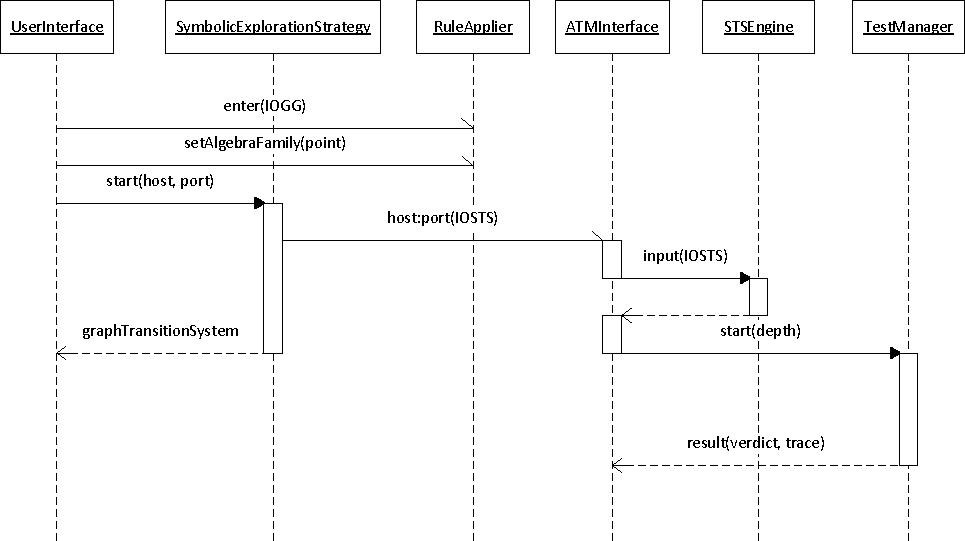
\includegraphics[width=\textwidth]{gratis_diagram.pdf}
  \end{center}
  \caption{GRATiS sequence diagram}
  \label{fig:tooling}
\end{figure}

\begin{enumerate}
\item The user enters an IOGG in the RuleApplier of the GROOVE tool. The input/output rules are defined by prefixing the given rule names with '?' and '!'. 
\item In the settings menu of GROOVE, the user sets the algebra family of the IOGG to to the point algebra, which is used by the RuleApplier.
\item The user selects the SymbolicExplorationStrategy from the available strategies in GROOVE. This strategy gives input options to a host name and port number. The strategy is then started by the user. The communication between the RuleApplier and the strategy is omitted here, this is the same as in the GROOVE diagram. The result of the exploration is an IOGTS under the point algebra.
\item The RemoteExplorationStrategy creates an IOSTS in Java objects from this IOGTS with the method described in chapter~\ref{chapter:gg_to_sts}. It then creates a message with the IOSTS and sends this message to the ATMInterface
\item The ATMInterface receives the message and gives the IOSTS to the STSEngine.
\item The ATMInterface starts the testing with the default `depth' parameter; making this configurable is not implemented yet. The communication between the TestManager, STSEngine and Adapter is omitted here.
\item The TestManager returns the test results to the ATMInterface. The test results are stored in a database and are viewable by starting the user interface of ATM (ommitted here).
\end{enumerate}

\section{Description of added functionality}\label{sec:added_func}
This section covers in detail the added functionality to GROOVE and ATM. 

\paragraph*{GROOVE exploration strategy}
Figure~\ref{fig:esi-diagram} shows the class diagram of the added exploration strategy interface. The RemoteExplorationStrategy extends a \textit{SymbolicStrategy}. The SymbolicExplorationStrategy has a \textit{closing} exploration strategy, which is a strategy that explores all graph states and rule transitions, such as the BreadthFirstStrategy.

The user starts the RemoteExplorationStrategy with a host and port, as described above. This strategy starts a ClosingStrategy. This strategy explores the IOGG and notifies the remote strategy when there are no more rule transitions to explore. The SymbolicStrategy implements  the method described in chapter~\ref{chapter:gg_to_sts} to build the IOSTS in Java objects using the explored IOGTS from the ClosingStrategy. The class diagram of this IOSTS is given in next.
 
\begin{figure}[ht]
  \begin{center}
    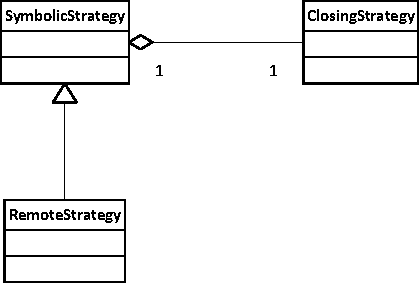
\includegraphics[width=0.35\textwidth]{strategy.pdf}
  \end{center}
  \caption{The class diagram of the exploration strategy interface}
  \label{fig:esi-diagram}
\end{figure}

\paragraph*{IOSTS in GROOVE}
Figure~\ref{fig:sts-diagram} shows the class diagram of the IOSTS in GRATiS. The IOSTS is composed of Location, SwitchRelation, Gate, Interaction- and LocationVariable classes. A Location object can be the start and target of any number of SwitchRelation objects. A SwitchRelation object has two Location objects; the start and target location. It also has one Gate object, which can belong to any number of SwitchRelation objects. A Gate object can have any number of InteractionVariable objects, but an InteractionVariable object belongs to only one Gate object. The IOSTS class has one singleton object, the RuleInspector, which contains the functionality of building guards and updates from rule graphs, i.e. the $\function_{\guard}$ and $\function_{\updateMapping}$ functions defined in~\ref{def:guard} and~\ref{def:um} respectively.

\begin{figure}[ht]
  \begin{center}
    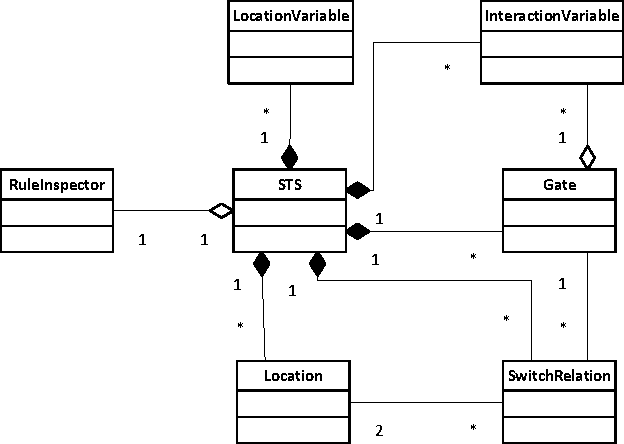
\includegraphics[width=0.5\textwidth]{STS.pdf}
  \end{center}
  \caption{The class diagram of the IOSTS in GRATiS}
  \label{fig:sts-diagram}
\end{figure}

Figure~\ref{fig:sts-objects} shows the object relations in accordance with the class diagram for the IOSTS in Figure~\ref{fig:example_sts}. Note that the links between the $\mathit{BoardGame}$ object and the Location, SwitchRelation, IOGate and InteractionVariable classes are not drawn for the sake of clarity. Note that the created objects, inter-object relations and object parameters are in accordance with the method described in chapter~\ref{chapter:gg_to_sts}. The IOSTS itself is the composite object, which also holds the initialization function. The RuleInspector is not part of the IOSTS, therefore the Boardgame object does not show the relation with this object.

\begin{figure}[ht]
  \begin{center}
    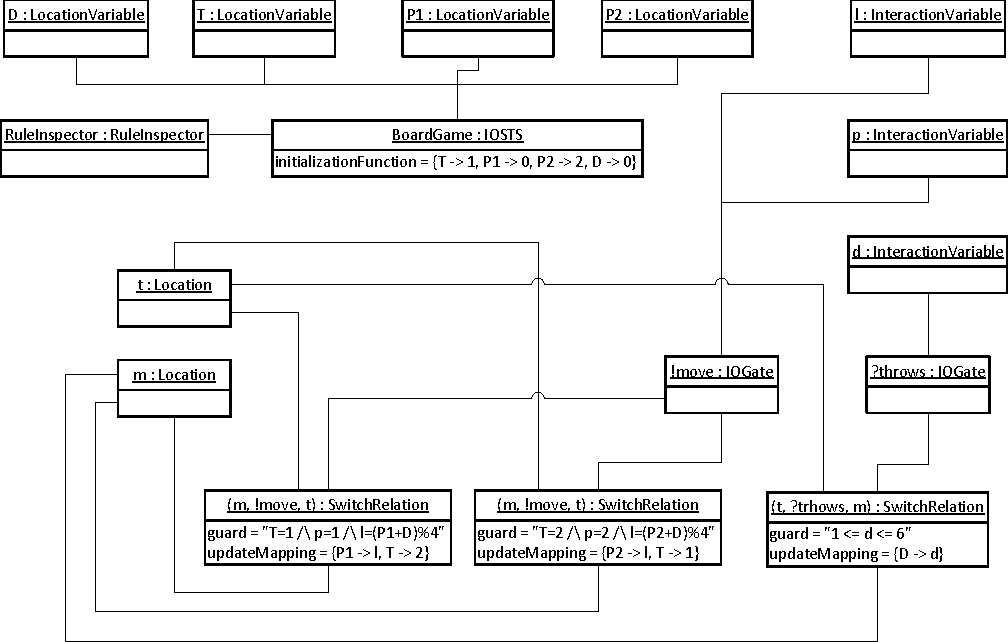
\includegraphics[width=0.8\textwidth]{STS_objects.pdf}
  \end{center}
  \caption{The object diagram of the IOSTS in Figure~\ref{fig:example_sts}}
  \label{fig:sts-objects}
\end{figure}

\paragraph*{GROOVE-ATM Interface}
The RemoteExplorationStrategy sends a HTTP POST request with the IOSTS in JSON format to the interface of ATM.
The ATM interface is one component in the Ruby on Rails framework. The interface is a controller in this Model-View-Controller framework. Controllers handle the HTTP requests given by the framework. The interface receives the IOSTS POST request, builds the IOSTS as Ruby objects and initiates the test using this IOSTS as model.

  \newpage
  \chapter{Validation}\label{chapter:validation}
  This chapter covers the validation of the design. The validation is done through case-studies, reported in section~\ref{sec:case-studies}. Measurements on models and the performance are reported in section~\ref{sec:measurements}.


  \section{Measurements}\label{sec:measurements}

This sections lists possible measurements on the models and execution of GRATiS on those models. For each measurement, a motivation is given for doing or not doing the measurement on the model examples and case study.

\subsection{Performance}
Performance in terms of execution time and 'heap-size' can be measured and compared.

\subsection{Simulation}
Does the transformation simulate the original STS? And vice versa?

\subsection{Error detection}
Introduce an error in model and see how fast GG and STS can find it. (mutation coverage)

\subsection{Coverage comparison}
Compare the Location/switch relation coverage of both the transformation and the original STS. Having a more complete STS is counter-beneficial here.

\subsection{Model complexity}
Halstead's software science op model complexity?

\subsection{Extendability}
Introduce a realistic scenario where functionality of the system is extended. Assess the needed changes to both models.

  \section{Example 1: boardgame}
The boardgame is the running example of which the IOSTS and IOGG are given in Figures~\ref{fig:example_sts} and \ref{fig:example_groove} respectively.

\subsection{Simulation and redundancy}
The responses used by the IOSTS and by the IOGG are different. Both models, used as examples to clarify the IOSTS and IOGG formalisms, were built with a different behavior in mind. Both allow a die to be thrown, after which the IOSTS directly moves the player to the correct location and passes the turn and the IOGG moves the player by a series of responses ended with a $!nextTurn$. Therefore, both IOSTSs do not simulate each other.

\subsection{Performance}
The IOSTS is generated in a runtime of 300 ms using a heap-size of 1.9 MB.

\subsection{Model complexity}
\begin{comment}
start:
13 distinct operands
1 distinct operator
33 operands
3 operators

move:
2 new distinct operands
5 new distinct operators
27 operands
6 operators

nextTurn:
0 new distinct operands
1 new distinct operator
13 operands
5 operators

throws:
3 new distinct operands
2 new distinct operators
30 operands
10 operators

$n_1 = 9, n_2 = 18, N_1 = 24, N_2 = 103$ 
 Volume is 127*4.75 = 603.25

IOSTS:
22 distinct operands
5 distinct operators
62 operands
25 operators

$n_1 = 5, n_2 = 22, N_1 = 25, N_2 = 62$
 Volume is 87*4.75 = 413.25
\end{comment}

Table~\ref{tab:halstead-bg} shows the measurements on the operators and operands of both models.\marginpar{lastig om te bepalen wat meegenomen moet worden. GGs hebben ook transition label, priority level, etc. Eigenlijk verborgen complexiteit}

\begin{table}[ht]
\begin{center}
\begin{tabular}{| l | c | c | c | c | c |}
  \hline
  & $n_1$ & $n_2$ & $N_1$ & $N_2$ & Volume \\ \hline
  IOGG & 9 & 18 & 24 & 103 & 603.25 \\ \hline
  IOSTS & 5 & 22 & 25 & 62 & 413.25 \\
  \hline
\end{tabular}
\end{center}
\caption{The Halstead measurements on the boardgame models}
\label{tab:halstead-bg}
\end{table}\marginpar{Heb hier eigenlijk vrij weinig over te zeggen. Conclusies komen later.}


\subsection{Extendability}
The boardgame is extended to include more players and locations. For the IOGG, this means adding new locations and players to the initial graph. The players get a fixed order in which they play. This means that the next turn rule also has to be extended. The result is in Figure~\ref{fig:gg-bg-extended}. This extension reduces the distinct number of operators by 1 and introduces no new operands. The number of operator occurences has decreased by 1 and the number of operand occurences has grown by 10.

\begin{figure}[ht]
  \begin{center}
    \subfloat[The initial graph]{\label{fig:start-bg-extended}% To use this figure in your LaTeX document
% import the package groove/resources/groove2tikz.sty
%
% Special colors
\begin{tikzpicture}[
% Special color styles
scale=\tikzscale]
\node[node] (n4)  at (2.200, -0.180) {\ml{\textbf{Player}\\id = 2}};
\node[node] (n12)  at (3.550, -0.615) {\ml{\textbf{Player}\\id = 3}};
\node[node] (n7)  at (2.180, -1.465) {\ml{\textbf{Location}}};
\node[node] (n11)  at (0.990, -0.600) {\ml{\textbf{Player}\\\textit{turn}\\id = 1}};
\node[node] (n8)  at (1.610, -2.765) {\ml{\textbf{Location}}};
\node[node] (n9)  at (0.930, -1.985) {\ml{\textbf{Location}}};
\node[node] (n10)  at (3.560, -2.025) {\ml{\textbf{Location}}};
\node[node] (n0)  at (4.820, -0.615) {\ml{\textbf{Die}\\rolls = 0}};
\node[node] (n6)  at (2.890, -2.760) {\ml{\textbf{Location}}};
\path[edge](n12.south -| 3.560, -2.025) -- node[lab]{at} (n10) ;
\path[edge] (n7)  -- node[lab]{next} (n10) ;
\path[edge] (n10)  -- node[lab]{next} (n6) ;
\path[edge] (n8)  -- node[lab]{next} (n9) ;
\path[edge](n11.south -| 0.930, -1.985) -- node[lab]{at} (n9) ;
\path[edge] (n9)  -- node[lab]{next} (n7) ;
\path[edge](n4.south -| 2.180, -1.465) -- node[lab]{at} (n7) ;
\path[edge] (n11)  -- node[lab]{next} (n4) ;
\path[edge] (n4)  -- node[lab]{next} (n12) ;
\path[edge](n12.west |- 0.990, -0.600) -- node[lab]{next} (n11) ;
\path[edge](n6.west |- 1.610, -2.765) -- node[lab]{next} (n8) ;
\userdefinedmacro
\end{tikzpicture}
\renewcommand{\userdefinedmacro}{\relax}
}\hspace{20px}
    \subfloat[The next turn rule]{\label{fig:nextTurn-bg-extended}% To use this figure in your LaTeX document
% import the package groove/resources/groove2tikz.sty
%
% Special colors
\begin{tikzpicture}[
% Special color styles
scale=\tikzscale]
\node[node] (n3)  at (1.075, -1.730) {\ml{\textbf{Die}\\rolls = 0}};
\node[node] (n2)  at (2.050, -0.660) {\ml{\textbf{Player}\\{\color{\green}\textit{$+$ turn}}}};
\node[node] (n0)  at (1.090, -0.650) {\ml{\textbf{Player}\\{\color{\blue}\textit{$-$ turn}}}};
\path[deledge](n0.south -| 1.075, -1.730) -- node[dellab]{throws} (n3) ;
\path[edge](n0.east |- 2.050, -0.660) -- node[lab]{next} (n2) ;
\userdefinedmacro
\end{tikzpicture}
\renewcommand{\userdefinedmacro}{\relax}
}
  \end{center}
  \caption{The extended graph grammar of the board game example in Figure~\ref{fig:example_groove}}
  \label{fig:gg-bg-extended}
\end{figure}

The IOSTS gains a variable and a switch relation for the new player. \begin{comment}The result is in Figure~\ref{fig:sts-bg-extended}.\end{comment} The distinct number of operators has not increased and the distinct number of operands has increased by 1. The number of operator occurences has increased by 9 and the number of operand occurences has increased by 17.

The volume of the IOGG has increased by 35.95. $n_1 = 8, n_2 = 18, N_1 = 23, N_2 = 113$ Volume is 136*4.70 = 639.20
The volume of the IOSTS has increased by 130.28. $n_1 = 5, n_2 = 23, N_1 = 34, N_2 = 79$ Volume is 113*4.81 = 543.53


\section{Example 2: farmer-wolf-goat-cabbage}
In this puzzle, a farmer, wolf, goat and cabbage are on one side of a river. The farmer can take upto one item to the other side. If the wolf and goat are on one side of the river without the farmer, the wolf eats the goat and the puzzle is reset. This also holds for the goat and the cabbage. The goal is to move all four to the other side of the river. The IOGG of this puzzle is in Figure~\ref{fig:gg-fwgc}. Here the 'move' and 'invalid' rules are similar, therefore only the 'move cabbage' rule is shown. The response rules '!retry', '!eaten' and '!done' have a higher priority. This ensures that a proper response is given after a move, before allowing more stimuli. The IOSTS of this puzzle is in Figure~\ref{fig:sts-fwgc}. It uses variables to keep track of the location of the items. These are checked to see if an invalid move is done, an item is being eaten or the puzzle has been completed.

\begin{figure}[ht]
  \begin{center}
    \subfloat[The initial graph]{\label{fig:start-bg}% To use this figure in your LaTeX document
% import the package groove/resources/groove2tikz.sty
%
% Special colors
\begin{tikzpicture}[
% Special color styles
scale=\tikzscale]
\node[node] (n8)  at (2.350, -0.680) {\ml{right}};
\node[node] (n3)  at (0.545, -1.010) {\ml{wolf}};
\node[node] (n4)  at (0.570, -1.370) {\ml{goat}};
\node[node] (n1)  at (2.355, -1.230) {\ml{bank}};
\node[node] (n5)  at (0.670, -1.730) {\ml{cabbage}};
\node[node] (n0)  at (1.555, -1.220) {\ml{bank}};
\node[node] (n7)  at (1.565, -0.680) {\ml{left}};
\node[node] (n2)  at (0.635, -0.680) {\ml{farmer}};
\path[edge] (n2)  -- node[lab]{at} (n0) ;
\path[edge] (n5)  -- node[lab]{at} (n0) ;
\path[edge] (n4)  -- node[lab]{at} (n0) ;
\path[edge](n1.north -| 2.350, -0.680) -- node[lab]{side} (n8) ;
\path[edge](n0.north -| 1.565, -0.680) -- node[lab]{side} (n7) ;
\path[edge] (n3)  -- node[lab]{at} (n0) ;
\userdefinedmacro
\end{tikzpicture}
\renewcommand{\userdefinedmacro}{\relax}
}\hspace{20px}
    \subfloat[The ?c (move cabbage) rule with priority 0]{\label{fig:c-fwgc}% To use this figure in your LaTeX document
% import the package groove/resources/groove2tikz.sty
%
% Special colors
\begin{tikzpicture}[
% Special color styles
scale=\tikzscale]
\node[node] (n1)  at (2.495, -1.015) {\ml{bank}};
\node[node] (n0)  at (0.945, -2.365) {\ml{bank}};
\node[node] (n3)  at (1.985, -1.975) {\ml{farmer}};
\node[node] (n4)  at (2.455, -2.365) {\ml{cabbage}};
\path[deledge](n4.west |- 0.945, -2.365) -- node[dellab]{at} (n0) ;
\path[deledge] (n3)  -- node[dellab]{at} (n0) ;
\path[newedge] (n3)  --  (n1) ;
\node[newlab] at (2.063, -1.303){at};
\path[newedge](n4.north -| 2.495, -1.015) -- node[newlab]{at} (n1) ;
\path[edge, -] (n0)  -- node[lab]{\textit{!=}} (n1) ;
\userdefinedmacro
\end{tikzpicture}
\renewcommand{\userdefinedmacro}{\relax}
}\\
    \subfloat[The ?c (invalid cabbage move) rule with priority 0]{\label{fig:c-invalid-fwgc}% To use this figure in your LaTeX document
% import the package groove/resources/groove2tikz.sty
%
% Special colors
\begin{tikzpicture}[
% Special color styles
scale=\tikzscale]
\node[newnode] (n5)  at (3.315, -1.515) {\ml{\textbf{InvalidMove}}};
\node[node] (n3)  at (1.025, -1.005) {\ml{farmer}};
\node[node] (n4)  at (2.085, -1.025) {\ml{cabbage}};
\node[node] (n1)  at (1.015, -1.525) {\ml{bank}};
\node[node] (n0)  at (2.065, -1.515) {\ml{bank}};
\path[edge](n3.south -| 1.015, -1.525) --  (n1) ;
\node[lab] at (1.020, -1.270){at};
\path[edge](n4.south -| 2.065, -1.515) -- node[lab]{at} (n0) ;
\path[edge, -](n1.east |- 2.065, -1.515) -- node[lab]{\textit{!=}} (n0) ;
\userdefinedmacro
\end{tikzpicture}
\renewcommand{\userdefinedmacro}{\relax}
}\hspace{20px}
    \subfloat[The !retry rule with priority 1]{\label{fig:retry-fwgc}% To use this figure in your LaTeX document
% import the package groove/resources/groove2tikz.sty
%
% Special colors
\begin{tikzpicture}[
% Special color styles
scale=\tikzscale]
\node[delnode] (n0)  at (1.155, -0.905) {\ml{\textbf{InvalidMove}}};
\userdefinedmacro
\end{tikzpicture}
\renewcommand{\userdefinedmacro}{\relax}
}\\
    \subfloat[The !eaten rule with priority 1]{\label{fig:reinit}% To use this figure in your LaTeX document
% import the package groove/resources/groove2tikz.sty
%
% Special colors
\begin{tikzpicture}[
% Special color styles
scale=\tikzscale]
\node[node] (n14)  at (4.815, -0.505) {\ml{bank}};
\node[node] (n17)  at (4.815, -1.945) {\ml{bank}};
\node[node] (n10)  at (3.795, -0.495) {\ml{farmer}};
\node[node] (n11)  at (3.750, -0.955) {\ml{wolf}};
\node[node] (n16)  at (4.755, -1.395) {\ml{bank}};
\node[node] (n8)  at (2.665, -1.180) {\ml{\textit{left}\\bank}};
\node[node] (n13)  at (3.815, -1.945) {\ml{cabbage}};
\node[node] (n5)  at (1.805, -1.165){};
\node[node] (n0)  at (1.805, -1.815) {\ml{farmer}};
\node[node] (n15)  at (4.825, -0.965) {\ml{bank}};
\node[node] (n1)  at (0.795, -1.815) {\ml{bank}};
\node[node] (n4)  at (0.795, -0.555){};
\node[node] (n3)  at (0.775, -1.175) {\ml{bank}};
\node[node] (n12)  at (3.715, -1.405) {\ml{goat}};
\path[edge](n4.south -| 0.775, -1.175) -- node[lab]{at} (n3) ;
\path[edge, -](n1.north -| 0.775, -1.175) -- node[lab]{\textit{!=}} (n3) ;
\path[deledge](n11.east |- 4.825, -0.965) -- node[dellab]{at} (n15) ;
\path[newedge] (n11)  -- node[newlab]{at}(n8.east |- 3.750, -0.955);
\path[deledge](n12.east |- 4.755, -1.395) -- node[dellab]{at} (n16) ;
\path[edge](n0.west |- 0.795, -1.815) -- node[lab]{at} (n1) ;
\path[newedge] (n13)  -- node[newlab]{at} (n8) ;
\path[deledge](n13.east |- 4.815, -1.945) -- node[dellab]{at} (n17) ;
\path[edge](n5.west |- 0.775, -1.175) -- node[lab]{at} (n3) ;
\path[newedge] (n10)  -- node[newlab]{at} (n8) ;
\path[deledge](n10.east |- 4.815, -0.505) -- node[dellab]{at} (n14) ;
\path[newedge] (n12)  -- node[newlab]{at}(n8.east |- 3.715, -1.405);
\path[edge] (n4)  -- node[lab]{eats} (n5) ;
\userdefinedmacro
\end{tikzpicture}
\renewcommand{\userdefinedmacro}{\relax}
}\\
    \subfloat[The !done rule with priority 1]{\label{fig:done}% To use this figure in your LaTeX document
% import the package groove/resources/groove2tikz.sty
%
% Special colors
\begin{tikzpicture}[
% Special color styles
scale=\tikzscale]
\node[node] (n2)  at (2.615, -2.685) {\ml{goat}};
\node[node] (n7)  at (1.305, -2.500) {\ml{\textit{left}\\bank}};
\node[node] (n0)  at (2.725, -1.915) {\ml{farmer}};
\node[node] (n1)  at (2.610, -2.295) {\ml{wolf}};
\node[node] (n4)  at (3.915, -2.475) {\ml{\textit{right}\\bank}};
\node[node] (n3)  at (2.755, -3.125) {\ml{cabbage}};
\path[newedge] (n1)  -- node[newlab]{at}(n7.east |- 2.610, -2.295);
\path[deledge] (n2)  -- node[dellab]{at}(n4.west |- 2.615, -2.685);
\path[newedge] (n3)  -- node[newlab]{at} (n7) ;
\path[deledge] (n3)  -- node[dellab]{at} (n4) ;
\path[deledge] (n0)  -- node[dellab]{at} (n4) ;
\path[newedge] (n0)  -- node[newlab]{at} (n7) ;
\path[deledge] (n1)  -- node[dellab]{at}(n4.west |- 2.610, -2.295);
\path[newedge] (n2)  -- node[newlab]{at}(n7.east |- 2.615, -2.685);
\userdefinedmacro
\end{tikzpicture}
\renewcommand{\userdefinedmacro}{\relax}
}
  \end{center}
  \caption{The graph grammar of the farmer-wolf-goat-cabbage puzzle}
  \label{fig:gg-fwgc}
\end{figure}

\begin{figure}[ht]
  \begin{center}
    $\xymatrix{
   \fbox{$l_0$} \ar@(ld,lu)[]^{?c\:|\:N=C\:|\:N:=!N;C:=!C} \ar@(dl,dr)[]_{!eaten\:|\:(N!=G\land G=C)\lor (N!=W\land W=G)\:|\:N:=false;W:=false;G:=false;C:=false} \ar@(ur,ul)[]_{!done\:|\:N\land W\land G\land C\:|\:N:=false;W:=false;G:=false;C:=false} \ar@/^/[rrrr]^{?c\:|\:N!=G\:|} &&&& \fbox{$l_1$} \ar@/^/[llll]^{!retry\:|\:true\:|}
}$

  \end{center}
  \caption{The IOSTS of the farmer-wolf-goat-cabbage puzzle}
  \label{fig:sts-fwgc}
\end{figure}\marginpar{STSen zijn eigenlijk niet weer te geven via dit soort diagrammen. Wellicht Tikz proberen, anders de STS opschrijven in de formele defnitie.}

\subsection{Simulation and redundancy}
Both the generated IOSTS and the IOSTS built by hand allow all inputs and give the appropriate responses when necessary. This shows that both IOSTSs simulate each other. The generated IOSTS has 50 switch relations and 0 location variables. The IOSTS built by hand has 11 switch relations and 4 location variables. The IOGG does not use variables to track the location of each item. Therefore the generated IOSTS has a location per state of the puzzle. 

\subsection{Performance}
The IOSTS is generated in a runtime of 770 ms using a heap-size of 5.2 MB.

\subsection{Model complexity}
\begin{comment}
start: 12 new operands, 26 operands
?c: 3 new operators, 0 new operands. 5 operators, 17 operands
?c-invalid: 0 new operators, 1 new operand. 2 operators, 14 operands
!retry: 0-0. 1 operator, 2 operands.
!eaten: 0-0. 9 operators, 36 operands
!done: 8 operators, 30 operands
\end{comment}

Table~\ref{tab:halstead-fwgc} shows the measurements on the operators and operands of both models.

\begin{table}[ht]
\begin{center}
\begin{tabular}{| l | c | c | c | c | c |}
  \hline
  & $n_1$ & $n_2$ & $N_1$ & $N_2$ & Volume \\ \hline
  IOGG & 3 & 13 & 25 & 125 & 498.29 \\ \hline
  IOSTS & 9 & 22 & 25 & 62 & 431.02 \\
  \hline
\end{tabular}
\end{center}
\caption{The Halstead measurements of the farmer-wolf-goat-cabbage puzzle}
\label{tab:halstead-fwgc}
\end{table}\marginpar{berekening heeft weggelaten regels en switch relations niet meegenomen}


\subsection{Extendability}
In another variant of this puzzle, when one of the items is eaten, the puzzle does not reset but undoes the last action. Figure~\ref{fig:gg-fwgc-extended} shows this extension in two rules: the 'move cabbage' and the 'eaten undo' rule. The rules keep track of the last moved items. When an item gets eaten, the last move can be undone.\marginpar{veranderde model complexity moet nog gegeven worden}\marginpar{Ik moet quantification nog uitleggen, in GROOVE}

\begin{figure}[ht]
  \begin{center}
    \subfloat[The move cabbage rule]{\label{fig:start-bg-extended}% To use this figure in your LaTeX document
% import the package groove/resources/groove2tikz.sty
%
% Special colors
\begin{tikzpicture}[
% Special color styles
scale=\tikzscale]
\node[node] (n1)  at (2.575, -2.515) {\ml{bank}};
\node[node] (n0)  at (1.345, -2.515) {\ml{bank}};
\node[node] (n3)  at (2.595, -1.385) {\ml{farmer}};
\node[quantnode] (n6)  at (2.525, -3.435) {\ml{$\forall$}};
\node[node] (n4)  at (1.395, -1.735) {\ml{cabbage}};
\node[node] (n5)  at (1.465, -3.425){};
\path[deledge](n4.south -| 1.345, -2.515) -- node[dellab]{at} (n0) ;
\path[deledge] (n5) .. controls (1.730, -3.140) and (1.690, -2.930) .. (1.690, -2.930).. controls (1.680, -2.880) and (1.380, -2.850) .. (1.360, -2.900).. controls (1.360, -2.900) and (1.270, -3.090) ..  (n5) ;
\node[dellab] at (1.529, -2.915){moved};
\path[deledge] (n3)  -- node[dellab]{at} (n0) ;
\path[quantedge](n5.east |- 2.525, -3.435) -- node[lab]{@} (n6) ;
\path[newedge](n3.south -| 2.575, -2.515) -- node[newlab]{at} (n1) ;
\path[newedge] (n4)  -- node[newlab]{at} (n1) ;
\path[edge, -](n0.east |- 2.575, -2.515) -- node[lab]{\textit{!=}} (n1) ;
\path[newedge] (n4) .. controls (1.600, -1.420) and (1.530, -1.220) .. (1.530, -1.220).. controls (1.510, -1.160) and (1.210, -1.180) .. (1.200, -1.230).. controls (1.200, -1.230) and (1.140, -1.440) ..  (n4) ;
\node[newlab] at (1.361, -1.225){moved};
\path[newedge] (n3) .. controls (2.800, -1.110) and (2.750, -0.940) .. (2.750, -0.940).. controls (2.730, -0.880) and (2.450, -0.880) .. (2.440, -0.930).. controls (2.440, -0.930) and (2.370, -1.100) ..  (n3) ;
\node[newlab] at (2.590, -0.935){moved};
\userdefinedmacro
\end{tikzpicture}
\renewcommand{\userdefinedmacro}{\relax}
}\hspace{20px}
    \subfloat[The eaten undo rule]{\label{fig:c-fwgc}% To use this figure in your LaTeX document
% import the package groove/resources/groove2tikz.sty
%
% Special colors
\begin{tikzpicture}[
% Special color styles
scale=\tikzscale]
\node[node] (n3)  at (0.785, -2.765) {\ml{bank}};
\node[node] (n4)  at (0.395, -1.095){};
\node[node] (n1)  at (2.725, -2.755) {\ml{bank}};
\node[node] (n6)  at (1.955, -1.885){};
\node[node] (n0)  at (2.715, -1.085) {\ml{farmer}};
\node[node] (n5)  at (1.505, -1.095){};
\node[quantnode] (n7)  at (2.265, -1.495) {\ml{$\forall$}};
\path[edge, -](n3.east |- 2.725, -2.755) -- node[lab]{\textit{!=}} (n1) ;
\path[edge](n0.south -| 2.725, -2.755) -- node[lab]{at} (n1) ;
\path[edge] (n5)  -- node[lab]{at} (n3) ;
\path[edge] (n4)  -- node[lab]{at} (n3) ;
\path[deledge] (n6)  -- node[dellab]{at} (n1) ;
\path[deledge] (n6) .. controls (1.700, -2.210) and (1.780, -2.430) .. (1.780, -2.430).. controls (1.790, -2.480) and (2.120, -2.480) .. (2.140, -2.430).. controls (2.140, -2.430) and (2.210, -2.210) ..  (n6) ;
\node[dellab] at (1.960, -2.430){moved};
\path[quantedge] (n6)  -- node[lab]{@} (n7) ;
\path[newedge] (n6)  -- node[newlab]{at} (n3) ;
\path[edge](n4.east |- 1.505, -1.095) -- node[lab]{eats} (n5) ;
\userdefinedmacro
\end{tikzpicture}
\renewcommand{\userdefinedmacro}{\relax}
}
  \end{center}
  \caption{The extended graph grammar of the farmer-wolf-goat-cabbage puzzle in Figure~\ref{fig:gg-fwgc}}
  \label{fig:gg-fwgc-extended}
\end{figure}\marginpar{Extended STS is ook nauwelijks weer te geven. Ik vraag me hier af ok ik niet gewoon de LTS moet geven, wellicht is die simpeler. De STS moet nu namelijk met variabelen de vorige posities van alle items bij gaan houden oid}

\section{Example 3: restaurant reservations}
Figure~\ref{fig:reservation_start} shows the initial graph of three tables at a restaurant and two potential customers. Figure~\ref{fig:make-reservation} shows part of a rule that allows people to make reservations. The start and end times are timestamps represented by integers. This rule allows people to make multiple reservations. However, this rule violates the constraint in section~\ref{sec:constraint-1}, because the reservation objects are not unique. Allowing a dynamic amount of reservations per person means that variables need to be introduced dynamically as well or more complex variables have to be used, such as arrays. To model this system using an IOSTS, arrays are also needed.

\begin{figure}[ht]
  \begin{center}
    \subfloat[The initial graph]{\label{fig:reservation_start}% To use this figure in your LaTeX document
% import the package groove/resources/groove2tikz.sty
%
% Special colors
\begin{tikzpicture}[
% Special color styles
scale=\tikzscale]
\node[node] (n2)  at (1.755, -1.545) {\ml{\textbf{Person}\\name = "Lisa Smith"}};
\node[node] (n1)  at (3.265, -1.535) {\ml{\textbf{Person}\\name = "John Doe"}};
\node[node] (n3)  at (2.540, -2.025) {\ml{\textbf{Table}\\number = 2}};
\node[node] (n5)  at (3.210, -2.585) {\ml{\textbf{Table}\\number = 3}};
\node[node] (n6)  at (1.860, -2.585) {\ml{\textbf{Table}\\number = 1}};
\userdefinedmacro
\end{tikzpicture}
\renewcommand{\userdefinedmacro}{\relax}
}\hspace{20px}
    \subfloat[The make reservation rule]{\label{fig:make-reservation}% To use this figure in your LaTeX document
% import the package groove/resources/groove2tikz.sty
%
% Special colors
\begin{tikzpicture}[
% Special color styles
scale=\tikzscale]
\node[node, attr] (n5)  at (2.070, -0.320) {\ml{\textbf{string}}};
\node[parnode] (n5p)  at (n5.north west) {0};
\node[node, attr] (n4)  at (3.580, -0.310) {\ml{\textbf{int}}};
\node[parnode] (n4p)  at (n4.north west) {1};
\node[node, attr] (n3)  at (3.650, -2.165) {\ml{\textbf{int}}};
\node[parnode] (n3p)  at (n3.north west) {3};
\node[node, attr] (n2)  at (2.030, -2.155) {\ml{\textbf{int}}};
\node[parnode] (n2p)  at (n2.north west) {2};
\node[node] (n1)  at (2.045, -0.915) {\ml{\textbf{Person}}};
\node[newnode] (n7)  at (2.815, -1.485) {\ml{\textbf{Reservation}}};
\node[node] (n0)  at (3.590, -0.920) {\ml{\textbf{Table}}};
\path[newedge] (n1)  -- node[newlab]{has} (n7) ;
\path[newedge] (n7)  -- node[newlab]{end\_time} (n3) ;
\path[newedge] (n7)  --  (n2) ;
\node[newlab] at (2.370, -1.780){start\_time};
\path[newedge] (n7)  -- node[newlab]{for} (n0) ;
\path[edge](n0.north -| 3.580, -0.310) -- node[lab]{number} (n4) ;
\path[edge](n1.north -| 2.070, -0.320) -- node[lab]{name} (n5) ;
\userdefinedmacro
\end{tikzpicture}
\renewcommand{\userdefinedmacro}{\relax}
}
  \end{center}
  \caption{The graph grammar of the restaurant reservation system}
  \label{fig:gg-reservation}
\end{figure}


\section{Example 4: bar tab system}
This example models a bar tab system, where customers can order beer, wine and soda. The price of the order adds to tab. Customers can pay their tab with money; they receive cash back if the payment exceeds the tab. The model is abstracted to include three customers. Furthermore, a customer can order only one drink. Drinks and payments are processed immediately before other drinks or payments can occur. The stimuli accepted by the system are $?o(i,d), ?p(i,p)$ for ordering a drink $d$ on bar tab $i$ and paying amount $p$ on bar tab $i$ respectively. The responses by the system are $!po(b), !pp(b,r)$ for processing an order giving the new bar tab balance $b$ and processing a payment giving the new account balance $b$ and the return funds $r$ respectively.

Figure~\ref{fig:gg-bartab} shows the IOGG of the bar tab system. The '!process\_order' and '!process\_payment' rule have a higher priority than the '?order' and '?pay' rule. Figure~\ref{fig:sts-bartab} shows the IOSTS of the bar tab system. The IOSTS uses the variables $T_1, T_2, T_3$ to keep track of the bar tabs of the three people. It uses the variables $I, P$ as temporary variables for the id and payment/price respectively. The function $m$ takes the maximum value of its parameters.

\begin{figure}[ht]
  \begin{center}
    \subfloat[The initial graph]{\label{fig:start-tab}% To use this figure in your LaTeX document
% import the package groove/resources/groove2tikz.sty
%
% Special colors
\begin{tikzpicture}[
% Special color styles
scale=\tikzscale]
\node[node] (n18)  at (2.965, -2.325) {\ml{\textbf{Payment}\\amount = 0.0}};
\node[node] (n13)  at (4.495, -0.815) {\ml{\textbf{Customer}\\\textit{customer3}\\id = 3\\tab = 0.0}};
\node[node] (n11)  at (3.015, -0.815) {\ml{\textbf{Customer}\\\textit{customer2}\\id = 2\\tab = 0.0}};
\node[node] (n9)  at (1.545, -0.815) {\ml{\textbf{Customer}\\\textit{customer1}\\id = 1\\tab = 0.0}};
\node[node] (n7)  at (4.395, -1.685) {\ml{\textbf{Drink}\\\textit{drink3}\\name = "wine"\\price = 2.10}};
\node[node] (n3)  at (2.895, -1.665) {\ml{\textbf{Drink}\\\textit{drink2}\\name = "beer"\\price = 1.50}};
\node[node] (n0)  at (1.405, -1.665) {\ml{\textbf{Drink}\\\textit{drink1}\\name = "coke"\\price = 0.80}};
\userdefinedmacro
\end{tikzpicture}
\renewcommand{\userdefinedmacro}{\relax}
}\\
    \subfloat[The ?o rule with priority 0]{\label{fig:order-tab}% To use this figure in your LaTeX document
% import the package groove/resources/groove2tikz.sty
%
% Special colors
\begin{tikzpicture}[
% Special color styles
scale=\tikzscale]
\node[node, attr] (n2)  at (3.175, -1.365) {\ml{\textbf{string}}};
\node[parnode] (n2p)  at (n2.north west) {1};
\node[node] (n0)  at (2.165, -1.365) {\ml{\textbf{Drink}}};
\node[node] (n1)  at (0.885, -1.355) {\ml{\textbf{Customer}}};
\node[node, attr] (n3)  at (0.860, -0.780) {\ml{\textbf{int}}};
\node[parnode] (n3p)  at (n3.north west) {0};
\path[edge](n0.east |- 3.175, -1.365) -- node[lab]{name} (n2) ;
\path[newedge](n1.east |- 2.165, -1.365) -- node[newlab]{orders} (n0) ;
\path[edge](n1.north -| 0.860, -0.780) -- node[lab]{id} (n3) ;
\userdefinedmacro
\end{tikzpicture}
\renewcommand{\userdefinedmacro}{\relax}
}\hspace{20px}
    \subfloat[The !po rule with priority 1]{\label{fig:process_order}% To use this figure in your LaTeX document
% import the package groove/resources/groove2tikz.sty
%
% Special colors
\begin{tikzpicture}[
% Special color styles
scale=\tikzscale]
\node[node, attr] (n5)  at (2.290, -2.255) {\ml{\textbf{real}}};
\node[parnode] (n5p)  at (n5.north west) {0};
\node[node, prod] (n4)  at (3.305, -2.825){};
\node[node, attr] (n3)  at (3.300, -1.555) {\ml{\textbf{real}}};
\node[node, attr] (n2)  at (1.170, -2.815) {\ml{\textbf{real}}};
\node[node] (n1)  at (1.185, -2.255) {\ml{\textbf{Drink}}};
\node[node] (n0)  at (1.175, -1.545) {\ml{\textbf{Customer}}};
\path[edge] (n4)  -- node[lab]{$\pi$0} (n3) ;
\path[deledge](n0.south -| 1.185, -2.255) -- node[dellab]{orders} (n1) ;
\path[newedge] (n0)  -- node[newlab]{tab} (n5) ;
\path[edge](n1.south -| 1.170, -2.815) -- node[lab]{price} (n2) ;
\path[edge] (n4)  -- node[lab]{add} (n5) ;
\path[edge] (n4)  -- node[lab]{$\pi$1} (n2) ;
\path[deledge](n0.east |- 3.300, -1.555) -- node[dellab]{tab} (n3) ;
\userdefinedmacro
\end{tikzpicture}
\renewcommand{\userdefinedmacro}{\relax}
}\\
    \subfloat[The ?p rule with priority 0]{\label{fig:pay-tab}% To use this figure in your LaTeX document
% import the package groove/resources/groove2tikz.sty
%
% Special colors
\begin{tikzpicture}[
% Special color styles
scale=\tikzscale]
\node[node, attr] (n4)  at (3.190, -1.975) {\ml{\textbf{real}}};
\node[node] (n3)  at (2.665, -1.195) {\ml{\textbf{Payment}}};
\node[node, attr] (n2)  at (0.975, -1.995) {\ml{\textbf{int}}};
\node[parnode] (n2p)  at (n2.north west) {0};
\node[node] (n0)  at (1.025, -1.215) {\ml{\textbf{Customer}}};
\node[node, attr] (n1)  at (2.040, -1.995) {\ml{\textbf{real}}};
\node[parnode] (n1p)  at (n1.north west) {1};
\path[deledge] (n3)  -- node[dellab]{amount} (n4) ;
\path[edge](n0.south -| 0.975, -1.995) -- node[lab]{id} (n2) ;
\path[newedge] (n3)  -- node[newlab]{amount} (n1) ;
\path[newedge](n0.east |- 2.665, -1.195) -- node[newlab]{pays} (n3) ;
\userdefinedmacro
\end{tikzpicture}
\renewcommand{\userdefinedmacro}{\relax}
}\hspace{20px}
    \subfloat[The !pp rule with priority 1]{\label{fig:process_payment}% To use this figure in your LaTeX document
% import the package groove/resources/groove2tikz.sty
%
% Special colors
\begin{tikzpicture}[
% Special color styles
scale=\tikzscale]
\node[node, attr] (n12)  at (1.150, -3.120) {\ml{\textbf{real}}};
\node[parnode] (n12p)  at (n12.north west) {1};
\node[node, attr] (n11)  at (3.510, -3.135) {\ml{\textbf{real}}};
\node[node, prod] (n10)  at (3.505, -2.475){};
\node[node, prod] (n9)  at (2.395, -3.125) {\ml{$\pi$0 = 0.0}};
\node[node, attr] (n8)  at (2.410, -1.815) {\ml{\textbf{real}}};
\node[node, prod] (n7)  at (2.405, -2.515) {\ml{$\pi$0 = 0.0}};
\node[node, prod] (n4)  at (3.515, -1.815){};
\node[node, attr] (n3)  at (1.260, -1.825) {\ml{\textbf{real}}};
\node[parnode] (n3p)  at (n3.north west) {0};
\node[node, attr] (n2)  at (2.460, -1.275) {\ml{\textbf{real}}};
\node[node, attr] (n1)  at (3.510, -1.255) {\ml{\textbf{real}}};
\node[node] (n0)  at (1.255, -0.735) {\ml{\textbf{Customer}}};
\node[node] (n5)  at (3.485, -0.745) {\ml{\textbf{Payment}}};
\path[edge] (n9)  -- node[lab]{$\pi$1} (n11) ;
\path[edge] (n4)  -- node[lab]{$\pi$1} (n1) ;
\path[edge](n5.south -| 3.510, -1.255) -- node[lab]{amount} (n1) ;
\path[edge] (n7)  -- node[lab]{max} (n3) ;
\path[edge] (n9)  -- node[lab]{max} (n12) ;
\path[edge] (n10)  -- node[lab]{neg} (n11) ;
\path[edge] (n7)  -- node[lab]{$\pi$1} (n8) ;
\path[edge] (n10)  -- node[lab]{$\pi$0} (n8) ;
\path[edge] (n4)  -- node[lab]{$\pi$0} (n2) ;
\path[deledge] (n0)  -- node[dellab]{tab} (n2) ;
\path[newedge](n0.south -| 1.260, -1.825) -- node[newlab]{tab} (n3) ;
\path[edge] (n4)  -- node[lab]{sub} (n8) ;
\path[deledge](n0.east |- 3.485, -0.745) -- node[dellab]{pays} (n5) ;
\userdefinedmacro
\end{tikzpicture}
\renewcommand{\userdefinedmacro}{\relax}
}
  \end{center}
  \caption{The graph grammar of the bar tab system}
  \label{fig:gg-bartab}
\end{figure}

\begin{figure}[ht]
  \begin{center}
    $\xymatrix{
   \ar[ddd]^<<<<{init\:|\:true\:|\:T_1:=0;T_2:=0;T_3:=0} \\ \\ \\
   \fbox{$l_0$} \ar[rrrrrrrrrr]|{?p(i, p)\:|\:1<=i\land i<=3\:|\:I:=i; P:=p} \ar@/_3pc/[ddrrrrrrrrrr]|{?o(i,o)\:|\:o="coke"\:|\:I:=i; P:=0.8} \ar@/_5pc/[ddrrrrrrrrrr]|{?o(i,o)\:|\:o="beer"\:|\:I:=i; P:=1.5} \ar@/_7pc/[ddrrrrrrrrrr]|{?o(i,o)\:|\:o="wine"\:|\:I:=i; P:=2.1} &&&&&&&&&& \fbox{$l_2$} \ar@/_1.5pc/[llllllllll]|{!pp(b, r)\:|\:I=1\land b=m(T_1-P,0)\land r=m(\scalebox{0.75}[1.0]{-}T_1+P,0)\:|\:T_1:=b} \ar@/_3pc/[llllllllll]|{!pp(b, r)\:|\:I=2\land b=m(T_2-P,0)\land r=m(\scalebox{0.75}[1.0]{-}T_2+P,0)\:|\:T_2:=b} \ar@/_5.2pc/[llllllllll]|{!pp(b, r)\:|\:I=3\land b=m(T_1-P,0)\land r=m(\scalebox{0.75}[1.0]{-}T_3+P,0)\:|\:T_3:=b} \\ \\
   &&&&&&&&&& \fbox{$l_1$} \ar@/^1.5pc/[uullllllllll]|{!po(b)\:|\:I=1\:|\:T_1:=T_1+P} \ar[uullllllllll]|{!po(b)\:|\:I=2\:|\:T_2:=T_2+P} \ar@/_1.5pc/[uullllllllll]|{!po(b)\:|\:I=3\:|\:T_3:=T_3+P} 
}$

  \end{center}
  \caption{The IOSTS of the bar tab system}
  \label{fig:sts-bartab}
\end{figure}

\subsection{Simulation and redundancy}
Both the generated IOSTS and the IOSTS built by hand correctly allow the ordering of drinks and payment of bar tabs. This shows that both IOSTSs simulate each other. The generated IOSTS has 24 switch relations and 13 location variables. The IOSTS built by hand has 10 switch relations and 5 location variables. This shows that the generated IOSTSs is redundant. The first IOSTS keeps the name and price of drinks as location variables, whereas the latter IOSTS hard-codes these into the guards and updates. The generated IOSTS builds a switch relation with gate $?o$ for each combination of customer and drink. It also builds a switch relation with gate $?p$ for each customer. The target locations of all these switch relations have one switch relation back to the initial location. Therefore, the number of switch relations is $3*3*2+3*1*2 = 24$.

\subsection{Performance}
The IOSTS is generated in a runtime of 250 ms using a heap-size of 2.1 MB.

\subsection{Model complexity}
\begin{comment}
start: 1 - 25. 13 - 46
?o: 1 - 2. 1 - 14
!po: 2 - 3. 4 - 24
?p: 0 - 0. 3 - 18
!pp: 3 - 
\end{comment}

Table~\ref{tab:halstead-bartab} shows the measurements on the operators and operands of both models.

\begin{table}[ht]
\begin{center}
\begin{tabular}{| l | c | c | c | c | c |}
  \hline
  & $n_1$ & $n_2$ & $N_1$ & $N_2$ & Volume \\ \hline
  IOGG & 3 & 13 & 25 & 125 & 498.29 \\ \hline
  IOSTS & 9 & 22 & 25 & 62 & 431.02 \\
  \hline
\end{tabular}
\end{center}
\caption{The Halstead measurements of the farmer-wolf-goat-cabbage puzzle}
\label{tab:halstead-bartab}
\end{table}\marginpar{moet nog even een abs in groove hebben, maakt uit voor deze berekening}


\subsection{Extendability}
The system is extended to allow ordering multiple drinks of different types. The stimulus \\$?o(i,d_1,q_1,d_2,q_2,d_3,q_3)$ is used to order a quantity $q_n$ of drink $d_n$. The bar tab id is still given by $i$. Also, a customer can purchase the option of receiving 10\% discount on all ordered drinks for 50 euros (added to the tab). The stimulus given is $?\mathit{d}$ and the response is $!pd(b)$ where $b$ is the new balance. Figure~\ref{fig:gg-bartab-extended} shows the extended rules and initial graph. The $?p$ and $!pp$ rules have remained the same.\marginpar{Deze GG en STS zijn vrij lelijk}

\begin{figure}[ht]
  \begin{center}
    \subfloat[The initial graph]{\label{fig:start-tab-extended}% To use this figure in your LaTeX document
% import the package groove/resources/groove2tikz.sty
%
% Special colors
\begin{tikzpicture}[
% Special color styles
scale=\tikzscale]
\node[node] (n18)  at (2.985, -2.905) {\ml{\textbf{Payment}\\amount = 0.0}};
\node[node] (n13)  at (4.495, -0.810) {\ml{\textbf{Customer}\\\textit{customer3}\\discount = 1.0\\id = 3\\tab = 0.0}};
\node[node] (n11)  at (3.015, -0.810) {\ml{\textbf{Customer}\\\textit{customer2}\\discount = 1.0\\id = 2\\tab = 0.0}};
\node[node] (n9)  at (1.545, -0.810) {\ml{\textbf{Customer}\\\textit{customer1}\\discount = 1.0\\id = 1\\tab = 0.0}};
\node[node] (n7)  at (4.415, -2.060) {\ml{\textbf{Drink}\\\textit{drink3}\\name = "wine"\\price = 2.10\\quantity = 0.0}};
\node[node] (n3)  at (2.915, -2.040) {\ml{\textbf{Drink}\\\textit{drink2}\\name = "beer"\\price = 1.50\\quantity = 0.0}};
\node[node] (n0)  at (1.425, -2.040) {\ml{\textbf{Drink}\\\textit{drink1}\\name = "coke"\\price = 0.80\\quantity = 0.0}};
\userdefinedmacro
\end{tikzpicture}
\renewcommand{\userdefinedmacro}{\relax}
}\hspace{20px}
    \subfloat[The !pd rule with priority 1]{\label{fig:process_discount}% To use this figure in your LaTeX document
% import the package groove/resources/groove2tikz.sty
%
% Special colors
\begin{tikzpicture}[
% Special color styles
scale=\tikzscale]
\node[node, attr] (n7)  at (2.240, -1.015) {\ml{\textbf{real}}};
\node[parnode] (n7p)  at (n7.north west) {0};
\node[node, prod] (n1)  at (1.545, -0.455) {\ml{$\pi$1 = 50.0}};
\node[node, attr] (n4)  at (0.800, -1.015) {\ml{\textbf{real}}};
\node[node, attr] (n5)  at (0.920, -2.605) {\ml{\textbf{real}}};
\node[node] (n2)  at (1.575, -1.880) {\ml{\textbf{Customer}\\{\color{\blue}$-$ request\_discount}\\{\color{\green}$+$ discount = 0.9}}};
\path[edge] (n1)  -- node[lab]{add} (n7) ;
\path[newedge] (n2)  -- node[newlab]{tab} (n7) ;
\path[deledge] (n2)  -- node[dellab]{tab} (n4) ;
\path[deledge] (n2)  -- node[dellab]{discount} (n5) ;
\path[edge] (n1)  -- node[lab]{$\pi$0} (n4) ;
\userdefinedmacro
\end{tikzpicture}
\renewcommand{\userdefinedmacro}{\relax}
}\\
    \subfloat[The extended ?o rule]{\label{fig:order-tab-extended}% To use this figure in your LaTeX document
% import the package groove/resources/groove2tikz.sty
%
% Special colors
\begin{tikzpicture}[
% Special color styles
scale=\tikzscale]
\node[node, attr] (n6)  at (2.380, -0.845) {\ml{\textbf{real}}};
\node[parnode] (n6p)  at (n6.north west) {2};
\node[node, attr] (n5)  at (1.130, -0.875) {\ml{\textbf{real}}};
\node[node] (n0)  at (1.775, -1.385) {\ml{\textbf{Drink}}};
\node[node] (n1)  at (2.935, -2.495) {\ml{\textbf{Customer}}};
\node[node, attr] (n3)  at (2.135, -2.495) {\ml{\textbf{int}}};
\node[parnode] (n3p)  at (n3.north west) {0};
\node[node, attr] (n2)  at (2.785, -1.385) {\ml{\textbf{string}}};
\node[parnode] (n2p)  at (n2.north west) {1};
\node[node, attr] (n7)  at (2.340, -4.065) {\ml{\textbf{real}}};
\node[parnode] (n7p)  at (n7.north west) {4};
\node[node, attr] (n9)  at (1.110, -4.065) {\ml{\textbf{real}}};
\node[node] (n4)  at (1.775, -3.435) {\ml{\textbf{Drink}}};
\node[node, attr] (n8)  at (2.785, -3.435) {\ml{\textbf{string}}};
\node[parnode] (n8p)  at (n8.north west) {3};
\node[node, attr] (n11)  at (4.760, -3.145) {\ml{\textbf{real}}};
\node[parnode] (n11p)  at (n11.north west) {6};
\node[node, attr] (n13)  at (3.530, -3.145) {\ml{\textbf{real}}};
\node[node] (n10)  at (4.195, -2.515) {\ml{\textbf{Drink}}};
\node[node, attr] (n12)  at (4.165, -1.945) {\ml{\textbf{string}}};
\node[parnode] (n12p)  at (n12.north west) {5};
\path[newedge] (n4)  -- node[newlab]{quantity} (n7) ;
\path[newedge](n1.east |- 4.195, -2.515) -- node[newlab]{orders} (n10) ;
\path[edge, -](n4.north -| 1.775, -1.385) -- node[lab]{\textit{!=}} (n0) ;
\path[newedge] (n0)  -- node[newlab]{quantity} (n6) ;
\path[edge, -] (n0)  -- node[lab]{\textit{!=}} (n10) ;
\path[newedge] (n10)  -- node[newlab]{quantity} (n11) ;
\path[deledge] (n10)  -- node[dellab]{quantity} (n13) ;
\path[newedge] (n1)  -- node[newlab]{orders} (n4) ;
\path[edge](n10.north -| 4.165, -1.945) -- node[lab]{name} (n12) ;
\path[edge](n4.east |- 2.785, -3.435) -- node[lab]{name} (n8) ;
\path[edge, -] (n4)  -- node[lab]{\textit{!=}} (n10) ;
\path[deledge] (n0)  -- node[dellab]{quantity} (n5) ;
\path[deledge] (n4)  -- node[dellab]{quantity} (n9) ;
\path[edge](n1.west |- 2.135, -2.495) -- node[lab]{id} (n3) ;
\path[edge](n0.east |- 2.785, -1.385) -- node[lab]{name} (n2) ;
\path[newedge] (n1)  -- node[newlab]{orders} (n0) ;
\userdefinedmacro
\end{tikzpicture}
\renewcommand{\userdefinedmacro}{\relax}
}\hspace{20px}
    \subfloat[The ?d rule with priority 0]{\label{fig:discount}% To use this figure in your LaTeX document
% import the package groove/resources/groove2tikz.sty
%
% Special colors
\begin{tikzpicture}[
% Special color styles
scale=\tikzscale]
\node[node] (n0)  at (1.305, -0.930) {\ml{\textbf{Customer}\\{\color{\green}\textit{$+$ request\_discount}}\\discount = 1.0}};
\node[node, attr] (n4)  at (2.505, -0.915) {\ml{\textbf{int}}};
\node[parnode] (n4p)  at (n4.north west) {0};
\path[edge](n0.east |- 2.505, -0.915) -- node[lab]{id} (n4) ;
\userdefinedmacro
\end{tikzpicture}
\renewcommand{\userdefinedmacro}{\relax}
}\\
    \subfloat[The extended !po rule]{\label{fig:process_order-extended}% To use this figure in your LaTeX document
% import the package groove/resources/groove2tikz.sty
%
% Special colors
\begin{tikzpicture}[
% Special color styles
scale=\tikzscale]
\node[node, attr] (n25)  at (3.435, -2.265) {\ml{\textbf{real}}};
\node[node, attr] (n24)  at (1.875, -2.285) {\ml{\textbf{real}}};
\node[node, prod] (n23)  at (3.935, -2.835){};
\node[node, prod] (n22)  at (2.395, -2.875){};
\node[node, attr] (n21)  at (5.040, -2.285) {\ml{\textbf{real}}};
\node[node, prod] (n20)  at (5.045, -3.445){};
\node[node, attr] (n19)  at (5.050, -3.995) {\ml{\textbf{real}}};
\node[node, attr] (n18)  at (3.940, -3.455) {\ml{\textbf{real}}};
\node[node, attr] (n17)  at (2.400, -3.505) {\ml{\textbf{real}}};
\node[node, prod] (n16)  at (1.485, -4.015){};
\node[node, attr] (n15)  at (0.740, -3.535) {\ml{\textbf{real}}};
\node[node, prod] (n14)  at (0.745, -2.855){};
\node[node, attr] (n13)  at (0.335, -2.295) {\ml{\textbf{real}}};
\node[node] (n11)  at (3.925, -1.725) {\ml{\textbf{Drink}}};
\node[node, attr] (n12)  at (4.390, -2.255) {\ml{\textbf{real}}};
\node[node] (n6)  at (2.355, -1.725) {\ml{\textbf{Drink}}};
\node[node, attr] (n10)  at (2.910, -2.275) {\ml{\textbf{real}}};
\node[node] (n0)  at (1.895, -1.055) {\ml{\textbf{Customer}}};
\node[node] (n1)  at (0.825, -1.745) {\ml{\textbf{Drink}}};
\node[node, attr] (n2)  at (1.280, -2.315) {\ml{\textbf{real}}};
\node[node, attr] (n3)  at (1.950, -0.425) {\ml{\textbf{real}}};
\node[node, prod] (n4)  at (3.835, -0.435){};
\node[node, attr] (n5)  at (2.990, -0.775) {\ml{\textbf{real}}};
\node[parnode] (n5p)  at (n5.north west) {0};
\node[node, attr] (n7)  at (3.980, -1.265) {\ml{\textbf{real}}};
\node[node, prod] (n8)  at (5.035, -1.545){};
\node[node, attr] (n9)  at (5.040, -0.895) {\ml{\textbf{real}}};
\path[edge] (n11)  -- node[lab]{quantity} (n25) ;
\path[edge] (n4)  -- node[lab]{add} (n5) ;
\path[edge] (n1)  -- node[lab]{price} (n2) ;
\path[edge] (n23)  -- node[lab]{add} (n18) ;
\path[edge] (n6)  --  (n24) ;
\node[lab] at (2.096, -2.013){quantity};
\path[edge] (n23)  -- node[lab]{$\pi$1} (n25) ;
\path[edge] (n22)  -- node[lab]{mul} (n17) ;
\path[edge] (n14)  -- node[lab]{$\pi$0} (n2) ;
\path[edge] (n16)  -- node[lab]{add} (n19) ;
\path[edge] (n8)  -- node[lab]{mul} (n9) ;
\path[edge] (n0)  -- node[lab]{discount} (n7) ;
\path[edge] (n14)  -- node[lab]{mul} (n15) ;
\path[edge] (n22)  -- node[lab]{$\pi$1} (n24) ;
\path[edge] (n16)  -- node[lab]{$\pi$1} (n17) ;
\path[edge] (n8)  -- node[lab]{$\pi$1} (n7) ;
\path[deledge] (n0)  -- node[dellab]{orders} (n6) ;
\path[edge] (n23)  -- node[lab]{$\pi$0} (n12) ;
\path[edge] (n8)  -- node[lab]{$\pi$0} (n21) ;
\path[deledge] (n0)  -- node[dellab]{orders} (n11) ;
\path[edge] (n20)  -- node[lab]{$\pi$0} (n19) ;
\path[newedge] (n0)  -- node[newlab]{tab} (n5) ;
\path[edge] (n11)  -- node[lab]{price} (n12) ;
\path[edge] (n22)  -- node[lab]{$\pi$0} (n10) ;
\path[deledge](n0.north -| 1.950, -0.425) -- node[dellab]{tab} (n3) ;
\path[edge] (n1)  -- node[lab]{quantity} (n13) ;
\path[edge] (n6)  -- node[lab]{price} (n10) ;
\path[edge] (n20)  -- node[lab]{$\pi$1} (n18) ;
\path[edge] (n4)  -- node[lab]{$\pi$1} (n9) ;
\path[edge] (n4)  -- node[lab]{$\pi$0} (n3) ;
\path[edge] (n14)  -- node[lab]{$\pi$1} (n13) ;
\path[deledge] (n0)  -- node[dellab]{orders} (n1) ;
\path[edge] (n16)  -- node[lab]{$\pi$0} (n15) ;
\path[edge] (n20)  -- node[lab]{add} (n21) ;
\userdefinedmacro
\end{tikzpicture}
\renewcommand{\userdefinedmacro}{\relax}
}\\
  \end{center}
  \caption{The extended graph grammar of the bar tab system}
  \label{fig:gg-bartab-extended}
\end{figure}

\begin{figure}[ht]
  \begin{center}
    $\xymatrix{
   \ar[ddd]^<<<<{init\:|\:true\:|\:T_1:=0;T_2:=0;T_3:=0;D_1:=1;D_2:=1;D_3:=1} \\ \\ \\
   \fbox{$l_0$} \ar[rrrrrrrrrr]|{?p(i, p)\:|\:i\%3=i\:|\:I:=i; P:=p} \ar@/_3pc/[ddrrrrrrrrrr]|{?o(i,o_1, q_1, o_2, q_2, o_3, q_3)\:|\:o_1="coke"\land o_2="beer"\land o_3="wine" \land q_1>0\land q_2>0\land q_3>0\land i\%3=i\:|\:I:=i; P:=0.8*q_1+1.5*q_2+2.1*q_3} &&&&&&&&&& \fbox{$l_2$} \ar@/_1.5pc/[llllllllll]|{!pp(b, r)\:|\:I=1\land b=m(T_1-P,0)\land r=m(\scalebox{0.75}[1.0]{-}T_1+P,0)\:|\:T_1:=b} \ar@/_3pc/[llllllllll]|{!pp(b, r)\:|\:I=2\land b=m(T_2-P,0)\land r=m(\scalebox{0.75}[1.0]{-}T_2+P,0)\:|\:T_2:=b} \ar@/_5.2pc/[llllllllll]|{!pp(b, r)\:|\:I=3\land b=m(T_1-P,0)\land r=m(\scalebox{0.75}[1.0]{-}T_3+P,0)\:|\:T_3:=b} \\ \\
   &&&&&&&&&& \fbox{$l_1$} \ar@/^1.5pc/[uullllllllll]|{!po(b)\:|\:I=1\:|\:T_1:=T_1+P*D_1} \ar[uullllllllll]|{!po(b)\:|\:I=2\:|\:T_2:=T_2+P*D_2} \ar@/_1.5pc/[uullllllllll]|{!po(b)\:|\:I=3\:|\:T_3:=T_3+P*D_3} 
}$

  \end{center}
  \caption{The extended IOSTS of the bar tab system}
  \label{fig:sts-bartab-extended}
\end{figure}


\section{Conclusions}
The simulation measurement in the boardgame example shows that not having a fixed specification leads to different behavior specified by the generated IOSTS. The translation of abstract stimuli and responses to the concrete stimuli and responses gives flexibility; an expected series of responses $!move(1) !move(1) !nextTurn$ can be translated from the concrete response $!move(1,2)$. However, this does give more work in the abstract to concrete stimuli/response translation. Also, the model does not reflect the specification precisely when using such a work-around.

The redundancy measurement reveals an interesting result in the bar tab example. Here, the possible morphisms of the rules on the graph lead to more switch relations than when the IOSTS is created by hand. This effect is common: in a GG, it is easy to represent the actors and rules specifying the interaction between these actors. The result is a switch relation for each combination of customer and drink. This is not a problem as long as the size of the generated IOSTS is manageable by GRATiS. If the number of switch relations becomes too great, creating the smaller IOSTS by hand also becomes unmanageable.

%The redundancy measurement also shows that for the farmer-wolf-goat-cabbage puzzle, the IOGG is easier expressed using no variables. 

It can be conlcuded that for these small examples the runtime and heap-size of the IOSTS generation are negligible. The results on the case study will show how this measurement scales using larger models.

Halstead conlcusions here.

Extendability conclusions here.

The lack of complex data structures, such as arrays, sets and objects is apparent from the restaurant reservation example. GGs inherently are Object-Oriented, which can be best seen in the bar tab example, where ids and tabs are combined, as well as names and prices. The lack of a summation operation in GROOVE causes the large GG of the extended bar tab system. Figure~\ref{fig:gg-tab-better} shows how this rule could look like. 

\begin{figure}[ht]
  \begin{center}
    % To use this figure in your LaTeX document
% import the package groove/resources/groove2tikz.sty
%
% Special colors
\begin{tikzpicture}[
% Special color styles
scale=\tikzscale]
\node[node, attr] (n9)  at (3.830, -0.975) {\ml{\textbf{real}}};
\node[node, prod] (n8)  at (3.845, -1.565){};
\node[node, attr] (n7)  at (3.000, -1.575) {\ml{\textbf{real}}};
\node[node, attr] (n5)  at (2.990, -0.775) {\ml{\textbf{real}}};
\node[parnode] (n5p)  at (n5.north west) {0};
\node[node, prod] (n4)  at (3.835, -0.435){};
\node[node, attr] (n3)  at (1.950, -0.425) {\ml{\textbf{real}}};
\node[node] (n0)  at (1.895, -1.055) {\ml{\textbf{Customer}}};
\node[node, attr] (n10)  at (2.760, -2.185) {\ml{\textbf{real}}};
\node[node] (n6)  at (1.895, -1.635) {\ml{\textbf{Drink}}};
\node[node, prod] (n16)  at (3.865, -3.415){};
\node[node, attr] (n17)  at (1.940, -3.415) {\ml{\textbf{real}}};
\node[node, attr] (n19)  at (3.870, -2.305) {\ml{\textbf{real}}};
\node[node, prod] (n22)  at (1.935, -2.785){};
\node[node, attr] (n24)  at (0.990, -2.175) {\ml{\textbf{real}}};
\node[quantnode] (n1)  at (1.930, -2.200) {\ml{$\forall$}};
\path[edge] (n8)  -- node[lab]{mul} (n9) ;
\path[edge] (n4)  -- node[lab]{$\pi$0} (n3) ;
\path[edge] (n22)  -- node[lab]{$\pi$1} (n24) ;
\path[edge] (n0)  -- node[lab]{discount} (n7) ;
\path[edge] (n22)  -- node[lab]{mul} (n17) ;
\path[edge] (n16)  -- node[lab]{real:sum} (n19) ;
\path[edge] (n4)  -- node[lab]{add} (n5) ;
\path[deledge](n0.south -| 1.895, -1.635) -- node[dellab]{orders} (n6) ;
\path[edge] (n6)  --  (n24) ;
\node[lab] at (1.633, -1.922){quantity};
\path[edge] (n6)  -- node[lab]{price} (n10) ;
\path[edge] (n16)  -- node[lab]{$\pi$0} (n17) ;
\path[edge] (n22)  -- node[lab]{$\pi$0} (n10) ;
\path[edge] (n8)  -- node[lab]{$\pi$0} (n19) ;
\path[deledge](n0.north -| 1.950, -0.425) -- node[dellab]{tab} (n3) ;
\path[edge] (n8)  -- node[lab]{$\pi$1} (n7) ;
\path[newedge] (n0)  -- node[newlab]{tab} (n5) ;
\path[edge] (n4)  -- node[lab]{$\pi$1} (n9) ;
\path[quantedge](n6.south -| 1.930, -2.200) -- node[lab]{@} (n1) ;
\path[quantedge](n10.west |- 1.930, -2.200) -- node[lab]{@} (n1) ;
\path[quantedge](n24.east |- 1.930, -2.200) -- node[lab]{@} (n1) ;
\path[quantedge] (n22)  -- node[lab]{@} (n1) ;
\path[quantedge] (n17) .. controls (2.270, -3.100) and (2.260, -2.490) ..  (n1) ;
\node[lab] at (2.268, -2.804){@};
\userdefinedmacro
\end{tikzpicture}
\renewcommand{\userdefinedmacro}{\relax}

  \end{center}
  \caption{A rule of the bar tab system containing the sum operation}
  \label{fig:gg-tab-better}
\end{figure}

  %\section{Measurements on examples}

\subsection{Simulation and redundancy}
Table~\ref{tab:simulation} shows the results for this measurement. It contains all examples in the `Example' column and `Model' contains `Generated' and `Modelled' to indicate which IOSTS counterpart of the example the measurements are for. The `Simulates?' column contains `Yes' if the model simulates its counterpart in the same example or `No' otherwise. `Switch relations' and `Location variables' give the number of these for each model. Using this information for both counterparts, the model is declared redundant or not in `Redundant', as described in definition~\ref{def:redundancy}. The results per example are discussed in the next paragraphs, followed by the conclusions for this measurement.

\begin{table}[ht]
\begin{center}
\begin{tabular}{|l|l|c|c|c|c|}
\hline
\textbf{Example} & \textbf{Model} & \textbf{Simulates?} & \textbf{$\Switches$} & \textbf{$\LocationVariables$} & \textbf{Redundant?} \\ \hline
Boardgame & Generated & No & 12 & 3 & - \\ \cline{2-6}
 & Modelled & No & 3 & 4 & - \\ \hline
FWGC & Generated & Yes & 50 & 0 & No \\ \cline{2-6}
 & Modelled & Yes & 11 & 4 & No \\ \hline
Bar tab & Generated IOSTS & Yes & 24 & 13 & Yes \\ \cline{2-6}
 & Modelled IOSTS & Yes & 10 & 5 & No \\ \hline
Reservations & Generated IOSTS & - & - & - & - \\ \cline{2-6}
 & Modelled IOSTS & - & - & - & - \\ \hline
SCRP & Generated IOSTS & Yes & 540 & 2 & No \\ \cline{2-6}
 & Modelled IOSTS & No & 1302 & 2 & Yes \\ \hline
\end{tabular}
\end{center}
\caption{Simulation and redundancy results}
\label{tab:simulation}
\end{table}

\paragraph*{Boardgame}
The responses used by the IOSTS and by the IOGG are different. Both models, used as examples to clarify the IOSTS and IOGG formalisms, were built with a different behavior in mind. Both allow a die to be thrown, after which the IOSTS directly moves the player to the correct location and passes the turn and the IOGG moves the player by a series of responses ended with a $!nextTurn$. Therefore, both IOSTSs do not simulate each other.

\paragraph*{FWGC}
The IOGG does not use variables to track the location of each item. Therefore, the generated IOSTS has a location per state of the puzzle. Since on neither side both the number of switch relations and location variables are higher, both models are not redundant.

\paragraph*{Bar-tab system}
The modelled IOSTS keeps the name and price of drinks as location variables, whereas the generated IOSTS hard-codes these into the guards and updates. The generated IOSTS builds a switch relation with gate $?o$ for each combination of customer and drink. It also builds a switch relation with gate $?p$ for each customer. The target locations of all these switch relations have one switch relation back to the initial location. Therefore, the number of switch relations is $3*3*2+3*1*2\: =\: 24$. This could have been avoided by modelling GG variables for the price and drinks. However, this would make the IOGG more complex. 

\paragraph*{SCRP}
The generated IOSTS allows every stimulus in every location. The modelled IOSTS is modelled to test a subset of the more interesting behavior. Therefore, the generated IOSTS simulates the modelled IOSTS, but not vice versa. The modelled IOSTS is also redundant, because it features many $\tau$ transitions.

\paragraph*{Conclusions}
This measurement shows that IOGGs are good at making a model input-complete. For the smaller examples, it shows that the modelled IOSTSs often have fewer locations than the generated IOSTSs. Presumably, when modelling with IOGGs, making rules that create new locations are preferred over adding GG variables, if possible.

\subsection{Model complexity}
Table~\ref{tab:halstead} shows the measurements on the operators and operands of all models.  The differences in complexity differ between the models. However, the $n_2$ and $N_1$ column jump out: the distinct number of operands is much higher for the IOGG models, but the total number of operators $N_1$ is much higher in the IOSTS models. This is based on the last three models, which express the same behavior.

\begin{table}[ht]
\begin{center}
\begin{tabular}{| l | l | c | c | c | c | c |}
  \hline
  \textbf{Example} & \textbf{Model} & $n_1$ & $n_2$ & $N_1$ & $N_2$ & Volume \\ \hline
  Boardgame & IOGG & 7 & 12 & 20 & 90 & 467.27 \\ \cline{2-7}
  & IOSTS & 6 & 9 & 14 & 27 & 160.18 \\ \hline
  FWGC & IOGG & 3 & 12 & 31 & 190 & 863.42 \\ \cline{2-7}
  & IOSTS & 6 & 8 & 103 & 130 & 887.11 \\ \hline
  Bar tab & IOGG & 9 & 31 & 40 & 188 & 1213.40 \\ \cline{2-7}
  & IOSTS & 8 & 15 & 66 & 134 & 904.7 \\ \hline
  Reservations & IOGG & 1 & 19 & 5 & 50 & 237.71 \\ \cline{2-7}
  & IOSTS & - & - & - & - & - \\ \hline
  SCRP & IOGG & 3 & 69 & 207 & 1506 & 10569.10 \\ \cline{2-7}
  & IOSTS & 3 & 6 & 730 & 2594 & 10536.83 \\ \hline
\end{tabular}
\end{center}
\caption{The Halstead measurements on the models}
\label{tab:halstead}
\end{table}

\subsection{Extendability}
The next paragraphs contain a hypothetical extension to each example. New models are given which feature the extension. In the last paragraph, the increase in model complexity for each example is given in a table. The restaurant reservation system is omitted from this measurement, as is SCRP.

\paragraph*{Boardgame}
The boardgame is extended to include one more player and one more location. For the IOGG, this means adding new locations and players to the initial graph. The players get a fixed order in which they play. This means that the next turn rule also has to be extended. The rest of the rules stay as they are. The extended rules are in Figure~\ref{fig:gg-bg-extended}.

\begin{figure}[ht]
  \begin{center}
    \subfloat[The initial graph]{\label{fig:start-bg-extended}% To use this figure in your LaTeX document
% import the package groove/resources/groove2tikz.sty
%
% Special colors
\begin{tikzpicture}[
% Special color styles
scale=\tikzscale]
\node[node] (n4)  at (2.200, -0.180) {\ml{\textbf{Player}\\id = 2}};
\node[node] (n12)  at (3.550, -0.615) {\ml{\textbf{Player}\\id = 3}};
\node[node] (n7)  at (2.180, -1.465) {\ml{\textbf{Location}}};
\node[node] (n11)  at (0.990, -0.600) {\ml{\textbf{Player}\\\textit{turn}\\id = 1}};
\node[node] (n8)  at (1.610, -2.765) {\ml{\textbf{Location}}};
\node[node] (n9)  at (0.930, -1.985) {\ml{\textbf{Location}}};
\node[node] (n10)  at (3.560, -2.025) {\ml{\textbf{Location}}};
\node[node] (n0)  at (4.820, -0.615) {\ml{\textbf{Die}\\rolls = 0}};
\node[node] (n6)  at (2.890, -2.760) {\ml{\textbf{Location}}};
\path[edge](n12.south -| 3.560, -2.025) -- node[lab]{at} (n10) ;
\path[edge] (n7)  -- node[lab]{next} (n10) ;
\path[edge] (n10)  -- node[lab]{next} (n6) ;
\path[edge] (n8)  -- node[lab]{next} (n9) ;
\path[edge](n11.south -| 0.930, -1.985) -- node[lab]{at} (n9) ;
\path[edge] (n9)  -- node[lab]{next} (n7) ;
\path[edge](n4.south -| 2.180, -1.465) -- node[lab]{at} (n7) ;
\path[edge] (n11)  -- node[lab]{next} (n4) ;
\path[edge] (n4)  -- node[lab]{next} (n12) ;
\path[edge](n12.west |- 0.990, -0.600) -- node[lab]{next} (n11) ;
\path[edge](n6.west |- 1.610, -2.765) -- node[lab]{next} (n8) ;
\userdefinedmacro
\end{tikzpicture}
\renewcommand{\userdefinedmacro}{\relax}
}\hspace{20px}
    \subfloat[The next turn rule]{\label{fig:nextTurn-bg-extended}% To use this figure in your LaTeX document
% import the package groove/resources/groove2tikz.sty
%
% Special colors
\begin{tikzpicture}[
% Special color styles
scale=\tikzscale]
\node[node] (n3)  at (1.075, -1.730) {\ml{\textbf{Die}\\rolls = 0}};
\node[node] (n2)  at (2.050, -0.660) {\ml{\textbf{Player}\\{\color{\green}\textit{$+$ turn}}}};
\node[node] (n0)  at (1.090, -0.650) {\ml{\textbf{Player}\\{\color{\blue}\textit{$-$ turn}}}};
\path[deledge](n0.south -| 1.075, -1.730) -- node[dellab]{throws} (n3) ;
\path[edge](n0.east |- 2.050, -0.660) -- node[lab]{next} (n2) ;
\userdefinedmacro
\end{tikzpicture}
\renewcommand{\userdefinedmacro}{\relax}
}
  \end{center}
  \caption{The extended IOGG of the board game example in Figure~\ref{fig:example_groove}}
  \label{fig:gg-bg-extended}
\end{figure}

The IOSTS gains a variable and a switch relation for the new player:
\vspace{5px} \\
$\begin{array}{lcl}
\Locations & = & \{t, m\} \\
\initialLocation & = & t \\
\LocationVariables & = & \{T, P1, P2, P3, D\} \\
\initializationFunction & = & \{T \mapsto 0, P1 \mapsto 0, P2 \mapsto 2, P3 \mapsto 0, D \mapsto 0\} \\
\InteractionVariables & = & \{d, p, l\} \\
\Gates & = & \{?throw, !move\} \\
\Switches & = & \{t\xrightarrow{?throw, 1 <= d <= 6, D \mapsto d}m, \\
 & & m\xrightarrow{!move, T=1 \land l=(P1+D)\%5, P1 \mapsto l, T \mapsto 2}t, \\
 & & m\xrightarrow{!move, T=2 \land l=(P2+D)\%5, P2 \mapsto l, T \mapsto 3}t, \\
 & & m\xrightarrow{!move, T=3 \land l=(P3+D)\%5, P3 \mapsto l, T \mapsto 1}t\}
\end{array}$

\paragraph*{FWGC}
In another variant of this puzzle, when one of the items is eaten, the puzzle can reset, but it can also undo the last action. The $\mathit{!eaten}$ rule can have either effect. In Figure~\ref{fig:gg-fwgc-extended} shows this extension for the IOGG in five rules. The rules keep track of the last moved items. When an item gets eaten, the last move can be undone.

The IOSTS in Figure~\ref{fig:sts-fwgc-extended} keeps extra variables for the previous positions of the items and adds one switch relation that restores the items to their previous positions when an item gets eaten.

\paragraph*{Bar tab system}
The system is extended to allow ordering multiple drinks of different types. Also, a customer can purchase the option of receiving 10\% discount on all ordered drinks for 50 euros, which is added to the tab of the customer.
\vspace{5px}
\begin{itemize}
\item $?o(i,d_1,q_1,d_2,q_2,d_3,q_3)$ is used to order a quantity $q_n$ of drink $d_n$ on bar tab $i$. 
\item $?d(i)$ is used to order the discount on bar tab $i$.
\item $!pd(b)$ process the discount where $b$ is the new balance. 
\end{itemize}
\vspace{5px}
Figure~\ref{fig:gg-bartab-extended} shows the extended rules and initial graph. The $?p$ and $!pp$ rules have remained the same. The bar tabs track their discount. When processing an order, the discount is applied to the total price.

The IOSTS in Figure~\ref{fig:sts-bartab-extended} gains three location variables to track the discount for each tab. An order discount and process discount switch relations are added. Like with the IOGG, the discount is applied to the total price of the ordered drinks.

\paragraph*{SCRP}
An extended version for the IOSTS of SCRP by Axini is not available as there is no extended version of the SUT. Creating an extended IOSTS for SCRP and a corresponding SUT is out of scope for this report. Therefore the extension measurement is not done on the models for SCRP.

\paragraph*{Model complexity increase}
Table~\ref{tab:halstead-extended} shows the measurements on the operators and operands of all extended models and the increase in model complexity. The differences in complexity differ between the models. The volume increase does not show one trend; it is much higher for the IOSTS in the farmer-wolf-goat-cabbage puzzle and much higher for the IOGG in the bar tab system.

\begin{table}[ht]
\begin{center}
\begin{tabular}{| l | l | c | c | c | c | c | c |}
  \hline
  \textbf{Example} & \textbf{Model} & $n_1$ & $n_2$ & $N_1$ & $N_2$ & Volume & Volume increase \\ \hline
  boardgame & IOGG & 6 & 12 & 20 & 105 & 521.24 & 53.97 \\ \cline{2-7}
  & IOSTS & 6 & 10 & 24 & 39 & 252.0 & 91.82\\ \hline
  FWGC & IOGG & 4 & 12 & 38 & 217 & 1020.00 & 156.58 \\ \cline{2-7}
  & IOSTS & 6 & 12 & 146 & 247 & 1638.78 & 751.67\\ \hline
  bar-tab system & IOGG & 9 & 36 & 65 & 290 & 1949.61 & 736.21 \\ \cline{2-7}
  & IOSTS & 8 & 23 & 88 & 156 & 1208.82 & 304.12 \\ \hline
  Reservations & IOGG & ?? & ?? & ?? & ?? & ?? \\ \cline{2-7}
  & IOSTS & - & - & - & - & - \\ \hline
\end{tabular}
\end{center}
\caption{The Halstead measurements on the extended models}
\label{tab:halstead-extended}
\end{table}

\begin{comment}
A recent extension on the protocol allows multiple accounts. While an account is not in state open, an idle account can be opened. This allows for a customer to scan his/her products, while another customer pays. Figure~\ref{fig:gg-fwgc-extended} shows the changes to the initial graph and the open account rules. Figure~\ref{fig:close-account-success-ext} shows the success response rule for closing an account: the order of closed accounts have to be kept, because the accounts have to be paid in that order.

\begin{figure}[ht]
  \begin{center}
    \subfloat[The initial graph]{\label{fig:start-scrp-ext}% To use this figure in your LaTeX document
% import the package groove/resources/groove2tikz.sty
%
% Special colors
\begin{tikzpicture}[
% Special color styles
scale=\tikzscale]
\node[node] (n0)  at (1.020, -1.065) {\ml{\textbf{CR}\\\textit{SS\_OFF}}};
\node[node] (n1)  at (2.520, -1.035) {\ml{\textbf{SFU}}};
\node[node] (n2)  at (1.025, -1.850) {\ml{\textbf{Account}\\\textit{AS\_IDLE}}};
\node[node] (n3)  at (2.055, -1.860) {\ml{\textbf{Account}\\\textit{AS\_IDLE}}};
\path[edge](n0.south -| 1.025, -1.850) -- node[lab]{has} (n2) ;
\path[edge] (n0)  -- node[lab]{has} (n3) ;
\userdefinedmacro
\end{tikzpicture}
\renewcommand{\userdefinedmacro}{\relax}
}\hspace{20px}
    \subfloat[The open account success rule]{\label{fig:open-account-success-ext}% To use this figure in your LaTeX document
% import the package groove/resources/groove2tikz.sty
%
% Special colors
\begin{tikzpicture}[
% Special color styles
scale=\tikzscale]
\node[node] (n2)  at (1.695, -0.770) {\ml{\textbf{CR}\\\textit{SS\_ON}}};
\node[node] (n0)  at (2.975, -1.975) {\ml{\textbf{Account}\\{\color{\blue}\textit{$-$ AS\_IDLE}}\\{\color{\green}\textit{$+$ AS\_OPEN}}}};
\node[node] (n11)  at (4.030, -0.775) {\ml{\textbf{SFU}}};
\node[delnode] (n3)  at (2.860, -0.770) {\ml{\textbf{Request}\\\textit{open}}};
\node[nacnode] (n1)  at (1.700, -2.030) {\ml{\textbf{Account}\\\textit{AS\_OPEN}}};
\path[edge] (n2)  -- node[lab]{has} (n0) ;
\path[nacedge](n2.south -| 1.700, -2.030) -- node[naclab]{has} (n1) ;
\path[deledge](n11.west |- 2.860, -0.770) -- node[dellab]{from} (n3) ;
\path[deledge](n3.west |- 1.695, -0.770) -- node[dellab]{to} (n2) ;
\userdefinedmacro
\end{tikzpicture}
\renewcommand{\userdefinedmacro}{\relax}
}\\
    \subfloat[The open account invalid rule]{\label{fig:open-account-invalid-ext}% To use this figure in your LaTeX document
% import the package groove/resources/groove2tikz.sty
%
% Special colors
\begin{tikzpicture}[
% Special color styles
scale=\tikzscale]
\node[node] (n2)  at (0.990, -0.875) {\ml{\textbf{CR}\\\textit{SS\_ON}}};
\node[node] (n1)  at (1.010, -1.940) {\ml{\textbf{Account}\\\textit{AS\_OPEN}}};
\node[node] (n11)  at (3.070, -0.875) {\ml{\textbf{SFU}}};
\node[delnode] (n0)  at (2.005, -0.890) {\ml{\textbf{Request}\\\textit{open}}};
\path[edge](n2.south -| 1.010, -1.940) -- node[lab]{has} (n1) ;
\path[deledge](n11.west |- 2.005, -0.890) -- node[dellab]{from} (n0) ;
\path[deledge](n0.west |- 0.990, -0.875) -- node[dellab]{to} (n2) ;
\userdefinedmacro
\end{tikzpicture}
\renewcommand{\userdefinedmacro}{\relax}
}\hspace{20px}
    \subfloat[The close account success rule]{\label{fig:close-account-success-ext}% To use this figure in your LaTeX document
% import the package groove/resources/groove2tikz.sty
%
% Special colors
\begin{tikzpicture}[
% Special color styles
scale=\tikzscale]
\node[delnode] (n8)  at (1.695, -0.760) {\ml{\textbf{Request}\\\textit{close}}};
\node[quantnode] (n4)  at (0.765, -2.515) {\ml{$\forall$}};
\node[node] (n2)  at (2.245, -2.505) {\ml{\textbf{Account}}};
\node[node] (n1)  at (0.740, -1.710) {\ml{\textbf{Account}\\\textit{AS\_CLOSED}}};
\node[node] (n0)  at (2.415, -1.705) {\ml{\textbf{Account}\\{\color{\blue}\textit{$-$ AS\_OPEN}}\\{\color{\green}\textit{$+$ AS\_CLOSED}}}};
\node[node] (n5)  at (0.595, -0.770) {\ml{\textbf{CR}\\\textit{SS\_ON}}};
\node[node] (n6)  at (2.820, -0.725) {\ml{\textbf{SFU}}};
\path[deledge](n6.west |- 1.695, -0.760) -- node[dellab]{from} (n8) ;
\path[quantedge](n1.south -| 0.765, -2.515) -- node[lab]{@} (n4) ;
\path[deledge](n8.west |- 0.595, -0.770) -- node[dellab]{to} (n5) ;
\path[nacedge] (n1)  -- node[naclab]{next} (n2) ;
\path[edge] (n5)  -- node[lab]{has} (n0) ;
\path[edge](n5.south -| 0.740, -1.710) -- node[lab]{has} (n1) ;
\path[newedge](n1.east |- 2.415, -1.705) -- node[newlab]{next} (n0) ;
\userdefinedmacro
\end{tikzpicture}
\renewcommand{\userdefinedmacro}{\relax}
}
  \end{center}
  \caption{Parts of the extended IOGG of Scanflow Cash Register Protocol}
  \label{fig:gg-fwgc-extended}
\end{figure}
\end{comment}

\subsection{Performance}
The performance of GRATiS on all models is in Table~\ref{tab:performance}.

\begin{table}[ht]
\begin{center}
\begin{tabular}{|l|c|c|}
\hline
\textbf{Example} & \textbf{runtime (ms)} & \textbf{heap-size (MB)} \\ \hline
Boardgame & 300 & 1.9 \\ \hline
FWGC & 770 & 5.2 \\ \hline
Bar tab & 250 & 2.1 \\ \hline
Reservations & - & - \\ \hline
SCRP & 9530 & 6.6 \\ \hline
\end{tabular}
\end{center}
\caption{Performance measurements}
\label{tab:performance}
\end{table}

The algorithm scales reasonably well; the IOGG of SCRP is on average 13 times more complex than the examples and the runtime is on average 23 times longer. The space usage also shows very little increase.
  
  \newpage
  \bibliography{bib/bibliography}{}
  \bibliographystyle{plain}

  \newpage
  \chapter*{List of Symbols\hfill} \addcontentsline{toc}{chapter}{List of Symbols}
  \listofsymbols

  \newpage
  \appendix
  \chapter{Farmer-Wolf-Goat-Cabbage IOGG}\label{app:fwgc}
  \begin{figure}[ht]
  \begin{center}
    \subfloat[The initial graph]{\label{fig:start-fwgc}% To use this figure in your LaTeX document
% import the package groove/resources/groove2tikz.sty
%
% Special colors
\begin{tikzpicture}[
% Special color styles
scale=\tikzscale]
\node[node] (n8)  at (2.350, -0.680) {\ml{right}};
\node[node] (n3)  at (0.545, -1.010) {\ml{wolf}};
\node[node] (n4)  at (0.570, -1.370) {\ml{goat}};
\node[node] (n1)  at (2.355, -1.230) {\ml{bank}};
\node[node] (n5)  at (0.670, -1.730) {\ml{cabbage}};
\node[node] (n0)  at (1.555, -1.220) {\ml{bank}};
\node[node] (n7)  at (1.565, -0.680) {\ml{left}};
\node[node] (n2)  at (0.635, -0.680) {\ml{farmer}};
\path[edge] (n2)  -- node[lab]{at} (n0) ;
\path[edge] (n5)  -- node[lab]{at} (n0) ;
\path[edge] (n4)  -- node[lab]{at} (n0) ;
\path[edge](n1.north -| 2.350, -0.680) -- node[lab]{side} (n8) ;
\path[edge](n0.north -| 1.565, -0.680) -- node[lab]{side} (n7) ;
\path[edge] (n3)  -- node[lab]{at} (n0) ;
\userdefinedmacro
\end{tikzpicture}
\renewcommand{\userdefinedmacro}{\relax}
}\hspace{20px}
    \subfloat[?n (priority 0)]{\label{fig:n-fwgc}% To use this figure in your LaTeX document
% import the package groove/resources/groove2tikz.sty
%
% Special colors
\begin{tikzpicture}[
% Special color styles
scale=\tikzscale]
\node[node] (n2)  at (2.015, -2.045) {\ml{farmer}};
\node[node] (n1)  at (2.045, -0.885) {\ml{bank}};
\node[node] (n0)  at (0.925, -2.035) {\ml{bank}};
\path[edge, -] (n0)  -- node[lab]{\textit{!=}} (n1) ;
\path[deledge](n2.west |- 0.925, -2.035) -- node[dellab]{at} (n0) ;
\path[newedge](n2.north -| 2.045, -0.885) -- node[newlab]{at} (n1) ;
\userdefinedmacro
\end{tikzpicture}
\renewcommand{\userdefinedmacro}{\relax}
} \\
    \subfloat[?w valid (priority 0)]{\label{fig:w-fwgc}% To use this figure in your LaTeX document
% import the package groove/resources/groove2tikz.sty
%
% Special colors
\begin{tikzpicture}[
% Special color styles
scale=\tikzscale]
\node[node] (n4)  at (2.305, -1.560) {\ml{wolf}};
\node[node] (n3)  at (1.745, -1.080) {\ml{farmer}};
\node[node] (n0)  at (0.955, -1.570) {\ml{bank}};
\node[node] (n1)  at (2.355, -0.560) {\ml{bank}};
\node[node] (n2)  at (0.920, -0.560){};
\path[newedge] (n3)  -- node[newlab]{at} (n1) ;
\path[deledge] (n3)  -- node[dellab]{at} (n0) ;
\path[nacedge](n1.west |- 0.920, -0.560) -- node[naclab]{side} (n2) ;
\path[edge](n0.north -| 0.920, -0.560) -- node[lab]{side} (n2) ;
\path[deledge](n4.west |- 0.955, -1.570) -- node[dellab]{at} (n0) ;
\path[newedge](n4.north -| 2.355, -0.560) -- node[newlab]{at} (n1) ;
\userdefinedmacro
\end{tikzpicture}
\renewcommand{\userdefinedmacro}{\relax}
}\hspace{20px}
    \subfloat[?w invalid (priority 0)]{\label{fig:w-invalid-fwgc}% To use this figure in your LaTeX document
% import the package groove/resources/groove2tikz.sty
%
% Special colors
\begin{tikzpicture}[
% Special color styles
scale=\tikzscale]
\node[node] (n0)  at (2.065, -1.515) {\ml{bank}};
\node[node] (n1)  at (1.015, -1.525) {\ml{bank}};
\node[node] (n4)  at (2.085, -1.025) {\ml{wolf}};
\node[node] (n3)  at (1.025, -1.005) {\ml{farmer}};
\node[newnode] (n5)  at (3.315, -1.515) {\ml{\textbf{InvalidMove}}};
\path[edge](n3.south -| 1.015, -1.525) --  (n1) ;
\node[lab] at (1.015, -1.265){at};
\path[edge](n4.south -| 2.065, -1.515) -- node[lab]{at} (n0) ;
\path[edge, -](n1.east |- 2.065, -1.515) -- node[lab]{\textit{!=}} (n0) ;
\userdefinedmacro
\end{tikzpicture}
\renewcommand{\userdefinedmacro}{\relax}
} \\
    \subfloat[?g valid (priority 0)]{\label{fig:g-fwgc}% To use this figure in your LaTeX document
% import the package groove/resources/groove2tikz.sty
%
% Special colors
\begin{tikzpicture}[
% Special color styles
scale=\tikzscale]
\node[node] (n2)  at (2.285, -0.915) {\ml{farmer}};
\node[node] (n1)  at (2.275, -2.205) {\ml{bank}};
\node[node] (n0)  at (0.855, -0.925) {\ml{bank}};
\node[node] (n3)  at (1.865, -1.275) {\ml{goat}};
\path[edge, -] (n0)  -- node[lab]{\textit{!=}} (n1) ;
\path[newedge] (n3)  -- node[newlab]{at} (n1) ;
\path[deledge] (n3)  -- node[dellab]{at} (n0) ;
\path[deledge](n2.west |- 0.855, -0.925) -- node[dellab]{at} (n0) ;
\path[newedge](n2.south -| 2.275, -2.205) -- node[newlab]{at} (n1) ;
\userdefinedmacro
\end{tikzpicture}
\renewcommand{\userdefinedmacro}{\relax}
}\hspace{20px}
    \subfloat[?g invalid (priority 0)]{\label{fig:g-invalid-fwgc}% To use this figure in your LaTeX document
% import the package groove/resources/groove2tikz.sty
%
% Special colors
\begin{tikzpicture}[
% Special color styles
scale=\tikzscale]
\node[newnode] (n5)  at (3.315, -1.515) {\ml{\textbf{InvalidMove}}};
\node[node] (n3)  at (1.025, -1.005) {\ml{farmer}};
\node[node] (n4)  at (2.085, -1.025) {\ml{goat}};
\node[node] (n1)  at (1.015, -1.525) {\ml{bank}};
\node[node] (n0)  at (2.065, -1.515) {\ml{bank}};
\path[edge](n3.south -| 1.015, -1.525) --  (n1) ;
\node[lab] at (1.015, -1.265){at};
\path[edge](n4.south -| 2.065, -1.515) -- node[lab]{at} (n0) ;
\path[edge, -](n1.east |- 2.065, -1.515) -- node[lab]{\textit{!=}} (n0) ;
\userdefinedmacro
\end{tikzpicture}
\renewcommand{\userdefinedmacro}{\relax}
} \\
    \subfloat[?c valid (priority 0)]{\label{fig:c-fwgc}% To use this figure in your LaTeX document
% import the package groove/resources/groove2tikz.sty
%
% Special colors
\begin{tikzpicture}[
% Special color styles
scale=\tikzscale]
\node[node] (n1)  at (2.495, -1.015) {\ml{bank}};
\node[node] (n0)  at (0.945, -2.365) {\ml{bank}};
\node[node] (n3)  at (1.985, -1.975) {\ml{farmer}};
\node[node] (n4)  at (2.455, -2.365) {\ml{cabbage}};
\path[deledge](n4.west |- 0.945, -2.365) -- node[dellab]{at} (n0) ;
\path[deledge] (n3)  -- node[dellab]{at} (n0) ;
\path[newedge] (n3)  --  (n1) ;
\node[newlab] at (2.063, -1.303){at};
\path[newedge](n4.north -| 2.495, -1.015) -- node[newlab]{at} (n1) ;
\path[edge, -] (n0)  -- node[lab]{\textit{!=}} (n1) ;
\userdefinedmacro
\end{tikzpicture}
\renewcommand{\userdefinedmacro}{\relax}
}\hspace{20px}
    \subfloat[?c invalid (priority 0)]{\label{fig:c-invalid-fwgc}% To use this figure in your LaTeX document
% import the package groove/resources/groove2tikz.sty
%
% Special colors
\begin{tikzpicture}[
% Special color styles
scale=\tikzscale]
\node[newnode] (n5)  at (3.315, -1.515) {\ml{\textbf{InvalidMove}}};
\node[node] (n3)  at (1.025, -1.005) {\ml{farmer}};
\node[node] (n4)  at (2.085, -1.025) {\ml{cabbage}};
\node[node] (n1)  at (1.015, -1.525) {\ml{bank}};
\node[node] (n0)  at (2.065, -1.515) {\ml{bank}};
\path[edge](n3.south -| 1.015, -1.525) --  (n1) ;
\node[lab] at (1.020, -1.270){at};
\path[edge](n4.south -| 2.065, -1.515) -- node[lab]{at} (n0) ;
\path[edge, -](n1.east |- 2.065, -1.515) -- node[lab]{\textit{!=}} (n0) ;
\userdefinedmacro
\end{tikzpicture}
\renewcommand{\userdefinedmacro}{\relax}
} \\
  \end{center}
  \end{figure}

  \begin{figure}[ht]
  \setcounter{subfigure}{8}
  \begin{center}
    \subfloat[!retry (priority 1)]{\label{fig:retry-fwgc}\parbox{4cm}{\centering% To use this figure in your LaTeX document
% import the package groove/resources/groove2tikz.sty
%
% Special colors
\begin{tikzpicture}[
% Special color styles
scale=\tikzscale]
\node[delnode] (n0)  at (1.155, -0.905) {\ml{\textbf{InvalidMove}}};
\userdefinedmacro
\end{tikzpicture}
\renewcommand{\userdefinedmacro}{\relax}
}}\\
    \subfloat[!eaten (priority 1)]{\label{fig:reinit}% To use this figure in your LaTeX document
% import the package groove/resources/groove2tikz.sty
%
% Special colors
\begin{tikzpicture}[
% Special color styles
scale=\tikzscale]
\node[node] (n14)  at (4.815, -0.505) {\ml{bank}};
\node[node] (n17)  at (4.815, -1.945) {\ml{bank}};
\node[node] (n10)  at (3.795, -0.495) {\ml{farmer}};
\node[node] (n11)  at (3.750, -0.955) {\ml{wolf}};
\node[node] (n16)  at (4.755, -1.395) {\ml{bank}};
\node[node] (n8)  at (2.665, -1.180) {\ml{\textit{left}\\bank}};
\node[node] (n13)  at (3.815, -1.945) {\ml{cabbage}};
\node[node] (n5)  at (1.805, -1.165){};
\node[node] (n0)  at (1.805, -1.815) {\ml{farmer}};
\node[node] (n15)  at (4.825, -0.965) {\ml{bank}};
\node[node] (n1)  at (0.795, -1.815) {\ml{bank}};
\node[node] (n4)  at (0.795, -0.555){};
\node[node] (n3)  at (0.775, -1.175) {\ml{bank}};
\node[node] (n12)  at (3.715, -1.405) {\ml{goat}};
\path[edge](n4.south -| 0.775, -1.175) -- node[lab]{at} (n3) ;
\path[edge, -](n1.north -| 0.775, -1.175) -- node[lab]{\textit{!=}} (n3) ;
\path[deledge](n11.east |- 4.825, -0.965) -- node[dellab]{at} (n15) ;
\path[newedge] (n11)  -- node[newlab]{at}(n8.east |- 3.750, -0.955);
\path[deledge](n12.east |- 4.755, -1.395) -- node[dellab]{at} (n16) ;
\path[edge](n0.west |- 0.795, -1.815) -- node[lab]{at} (n1) ;
\path[newedge] (n13)  -- node[newlab]{at} (n8) ;
\path[deledge](n13.east |- 4.815, -1.945) -- node[dellab]{at} (n17) ;
\path[edge](n5.west |- 0.775, -1.175) -- node[lab]{at} (n3) ;
\path[newedge] (n10)  -- node[newlab]{at} (n8) ;
\path[deledge](n10.east |- 4.815, -0.505) -- node[dellab]{at} (n14) ;
\path[newedge] (n12)  -- node[newlab]{at}(n8.east |- 3.715, -1.405);
\path[edge] (n4)  -- node[lab]{eats} (n5) ;
\userdefinedmacro
\end{tikzpicture}
\renewcommand{\userdefinedmacro}{\relax}
}\\
    \subfloat[!done (priority 1)]{\label{fig:done}% To use this figure in your LaTeX document
% import the package groove/resources/groove2tikz.sty
%
% Special colors
\begin{tikzpicture}[
% Special color styles
scale=\tikzscale]
\node[node] (n2)  at (2.615, -2.685) {\ml{goat}};
\node[node] (n7)  at (1.305, -2.500) {\ml{\textit{left}\\bank}};
\node[node] (n0)  at (2.725, -1.915) {\ml{farmer}};
\node[node] (n1)  at (2.610, -2.295) {\ml{wolf}};
\node[node] (n4)  at (3.915, -2.475) {\ml{\textit{right}\\bank}};
\node[node] (n3)  at (2.755, -3.125) {\ml{cabbage}};
\path[newedge] (n1)  -- node[newlab]{at}(n7.east |- 2.610, -2.295);
\path[deledge] (n2)  -- node[dellab]{at}(n4.west |- 2.615, -2.685);
\path[newedge] (n3)  -- node[newlab]{at} (n7) ;
\path[deledge] (n3)  -- node[dellab]{at} (n4) ;
\path[deledge] (n0)  -- node[dellab]{at} (n4) ;
\path[newedge] (n0)  -- node[newlab]{at} (n7) ;
\path[deledge] (n1)  -- node[dellab]{at}(n4.west |- 2.610, -2.295);
\path[newedge] (n2)  -- node[newlab]{at}(n7.east |- 2.615, -2.685);
\userdefinedmacro
\end{tikzpicture}
\renewcommand{\userdefinedmacro}{\relax}
}
  \end{center}
  \end{figure}


  \newpage
  \chapter{Scanflow Cash Register Specification}\label{app:scrp-specification}

  \newpage
  \chapter{Scanflow Cash Register Models}\label{app:scrp-gg}
\end{document}
